\section{Fake round-10 key correlation plots}
\label{app:task1-plots}
Figure~\ref{fig:task1-example} shows byte 0. The following plots cover bytes 1 through 15.

\begin{figure}[H]
\centering
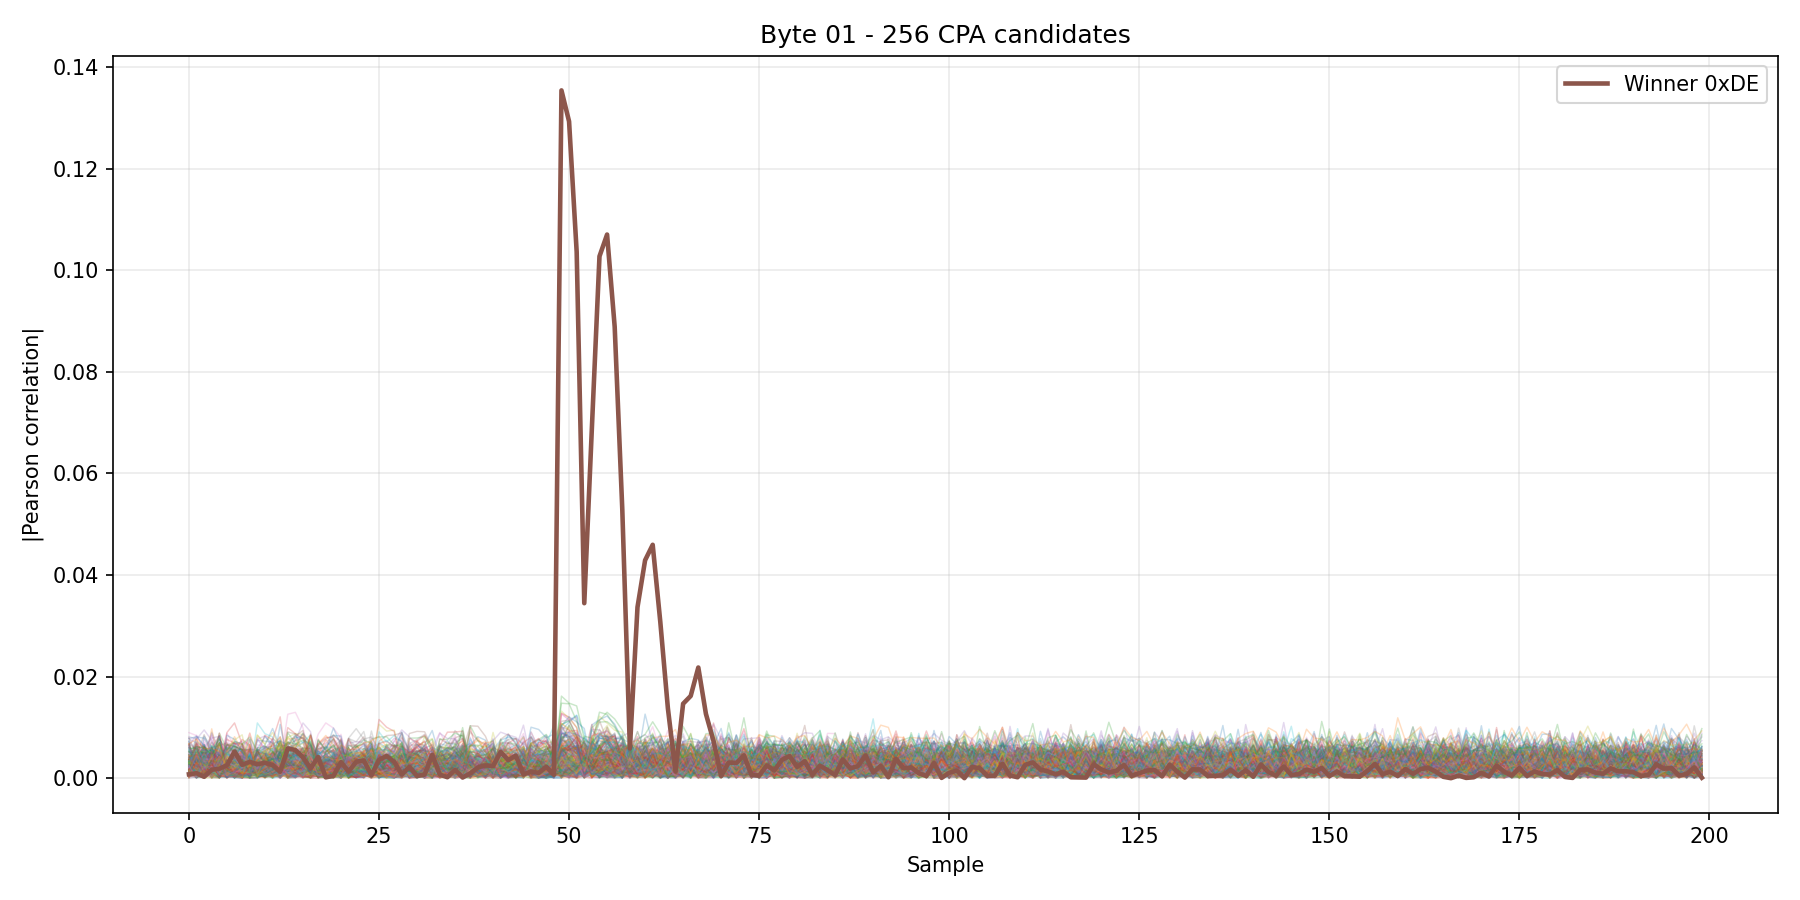
\includegraphics[width=0.92\textwidth]{correlation_plots_full/byte_01.png}
\caption{Task 1: absolute CPA correlations for all 256 candidates at byte 01. The thick curve marks the winning candidate.}
\label{fig:task1-byte-01}
\end{figure}

\begin{figure}[H]
\centering
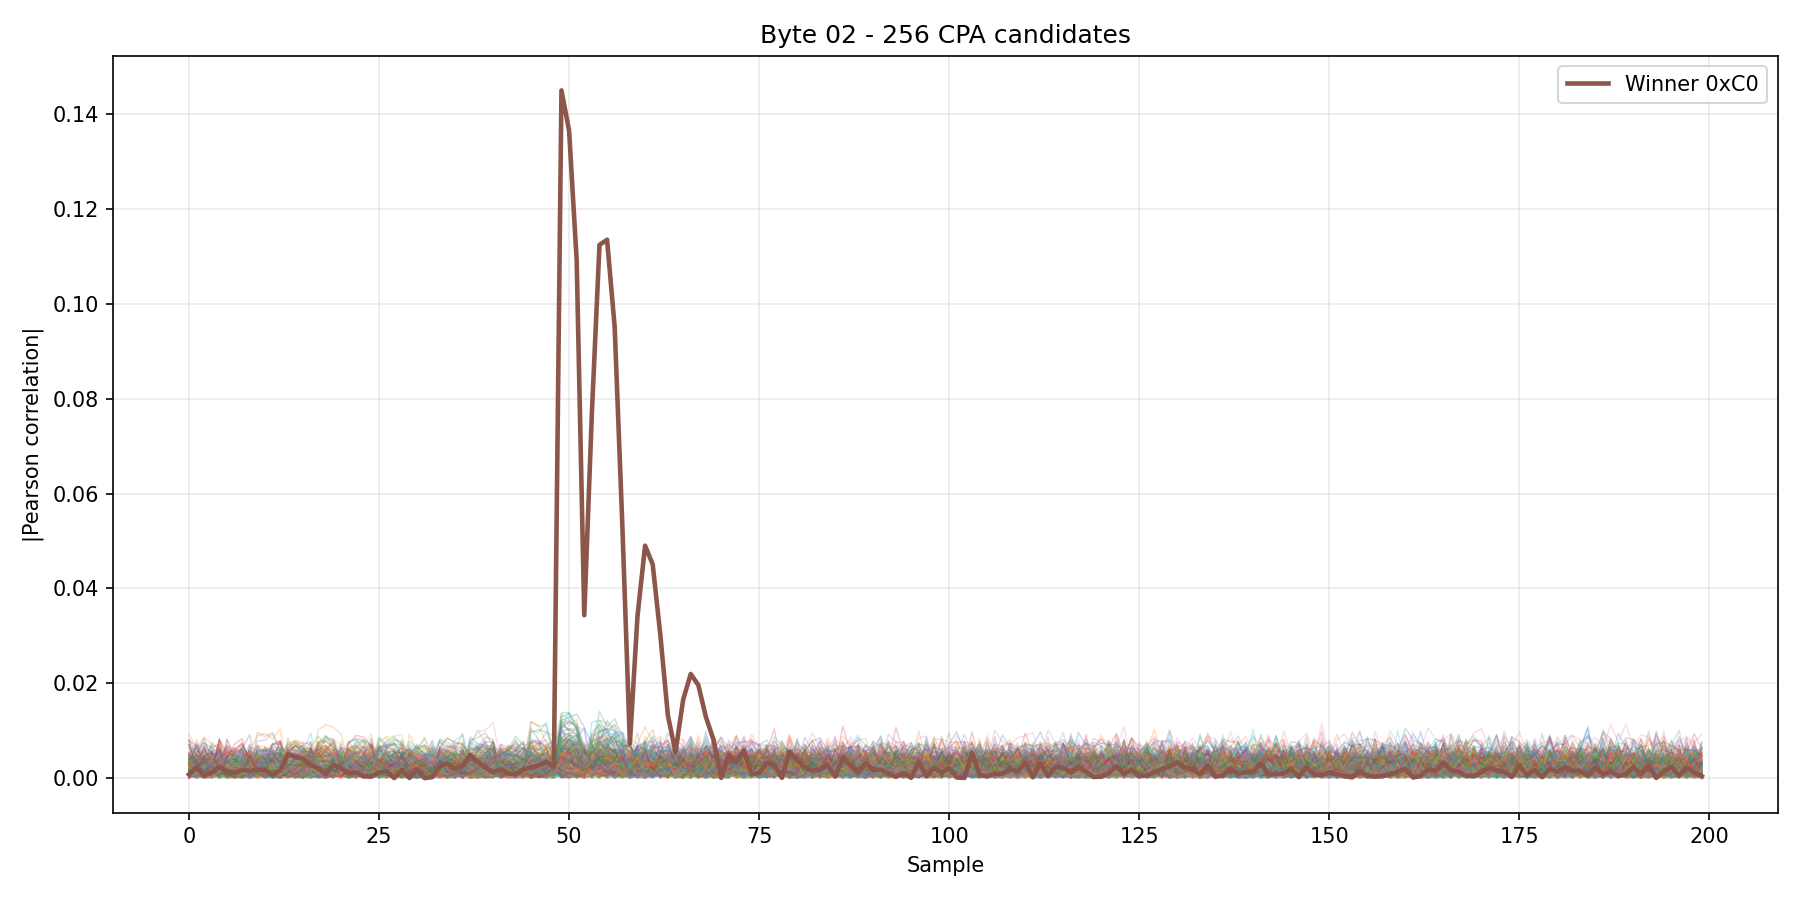
\includegraphics[width=0.92\textwidth]{correlation_plots_full/byte_02.png}
\caption{Task 1: absolute CPA correlations for all 256 candidates at byte 02. The thick curve marks the winning candidate.}
\label{fig:task1-byte-02}
\end{figure}

\clearpage

\begin{figure}[H]
\centering
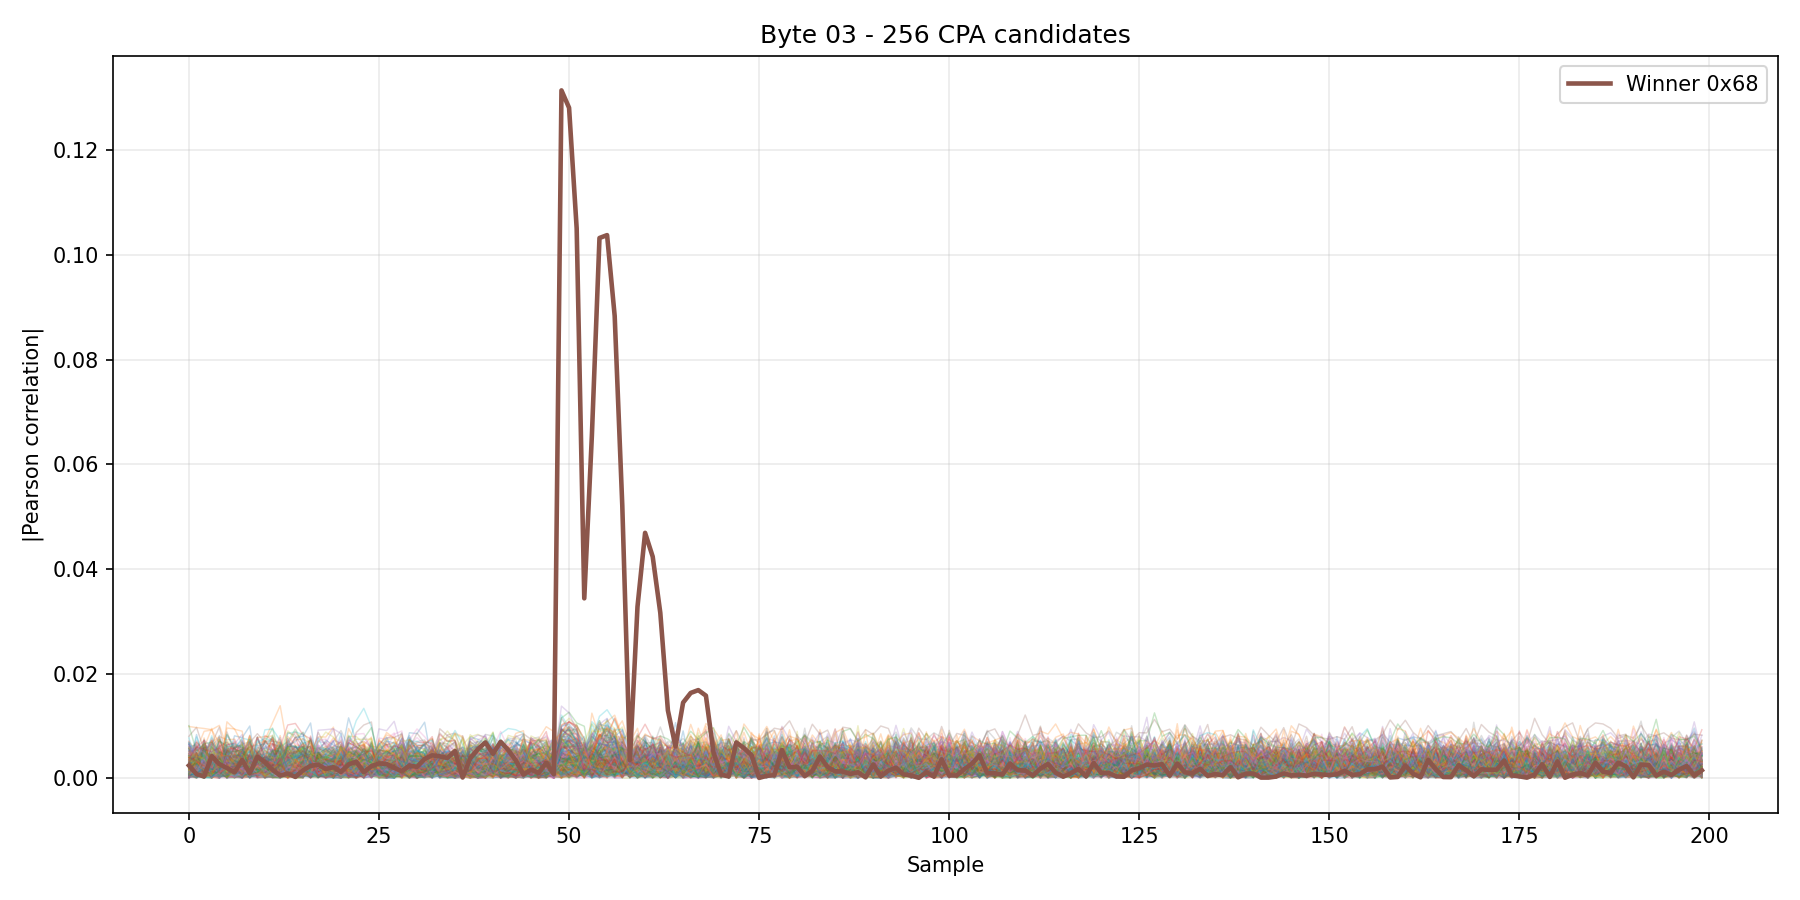
\includegraphics[width=0.92\textwidth]{correlation_plots_full/byte_03.png}
\caption{Task 1: absolute CPA correlations for all 256 candidates at byte 03. The thick curve marks the winning candidate.}
\label{fig:task1-byte-03}
\end{figure}

\begin{figure}[H]
\centering
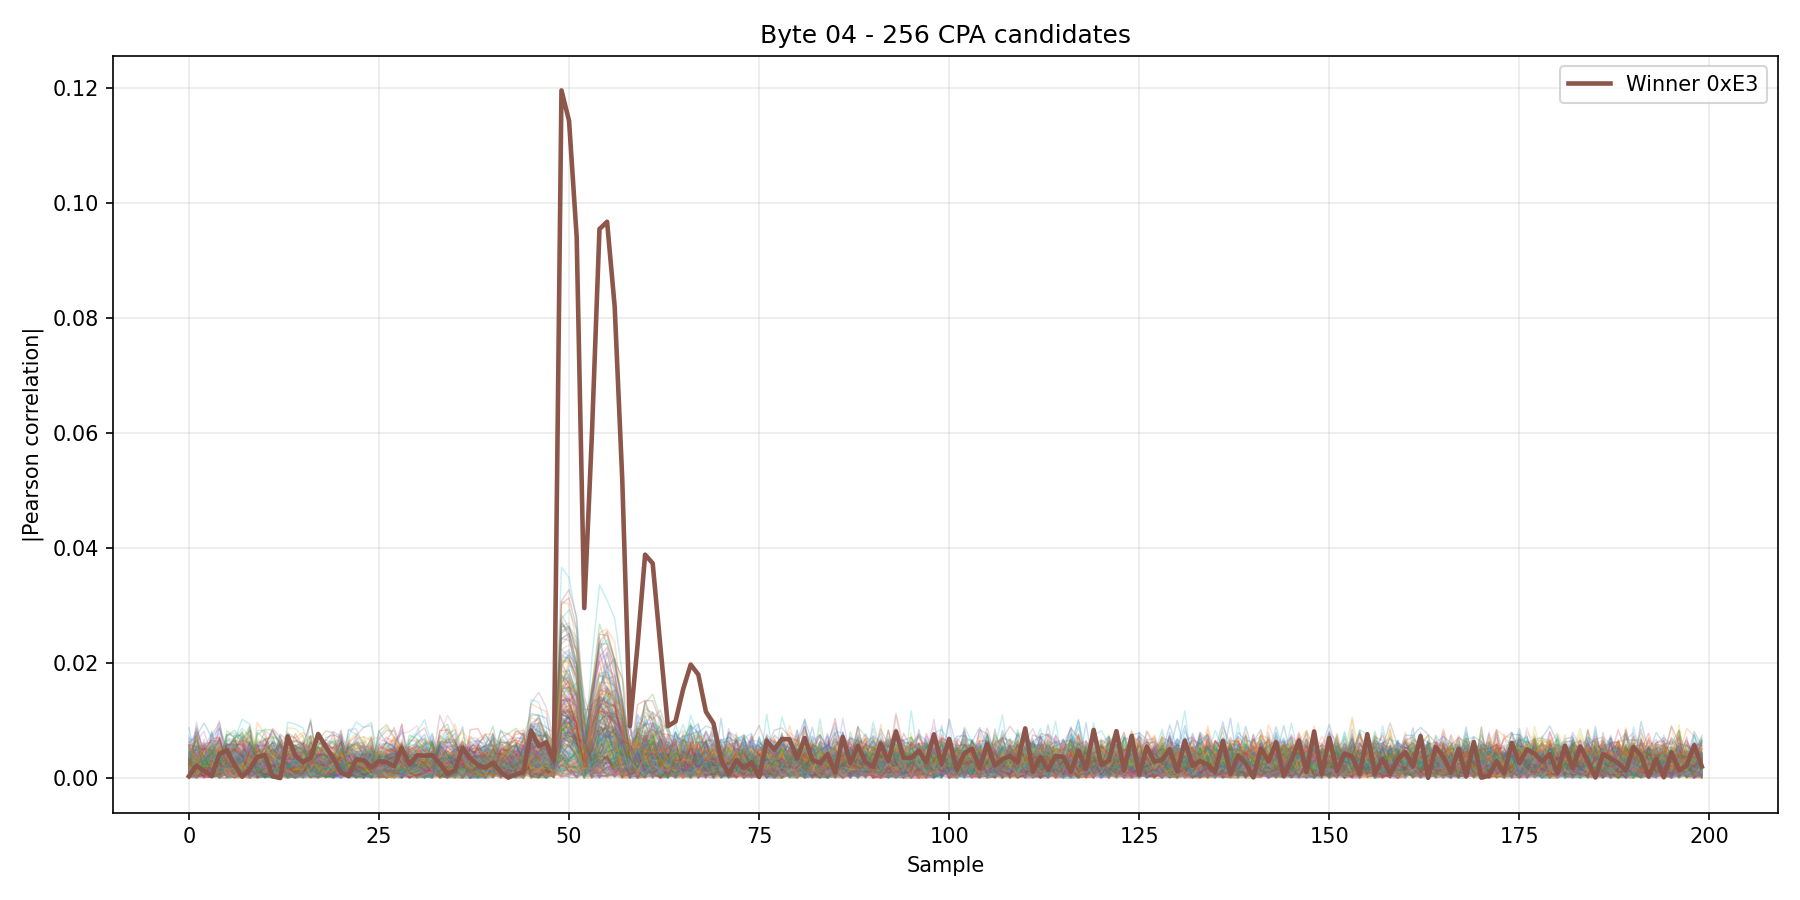
\includegraphics[width=0.92\textwidth]{correlation_plots_full/byte_04.png}
\caption{Task 1: absolute CPA correlations for all 256 candidates at byte 04. The thick curve marks the winning candidate.}
\label{fig:task1-byte-04}
\end{figure}

\clearpage

\begin{figure}[H]
\centering
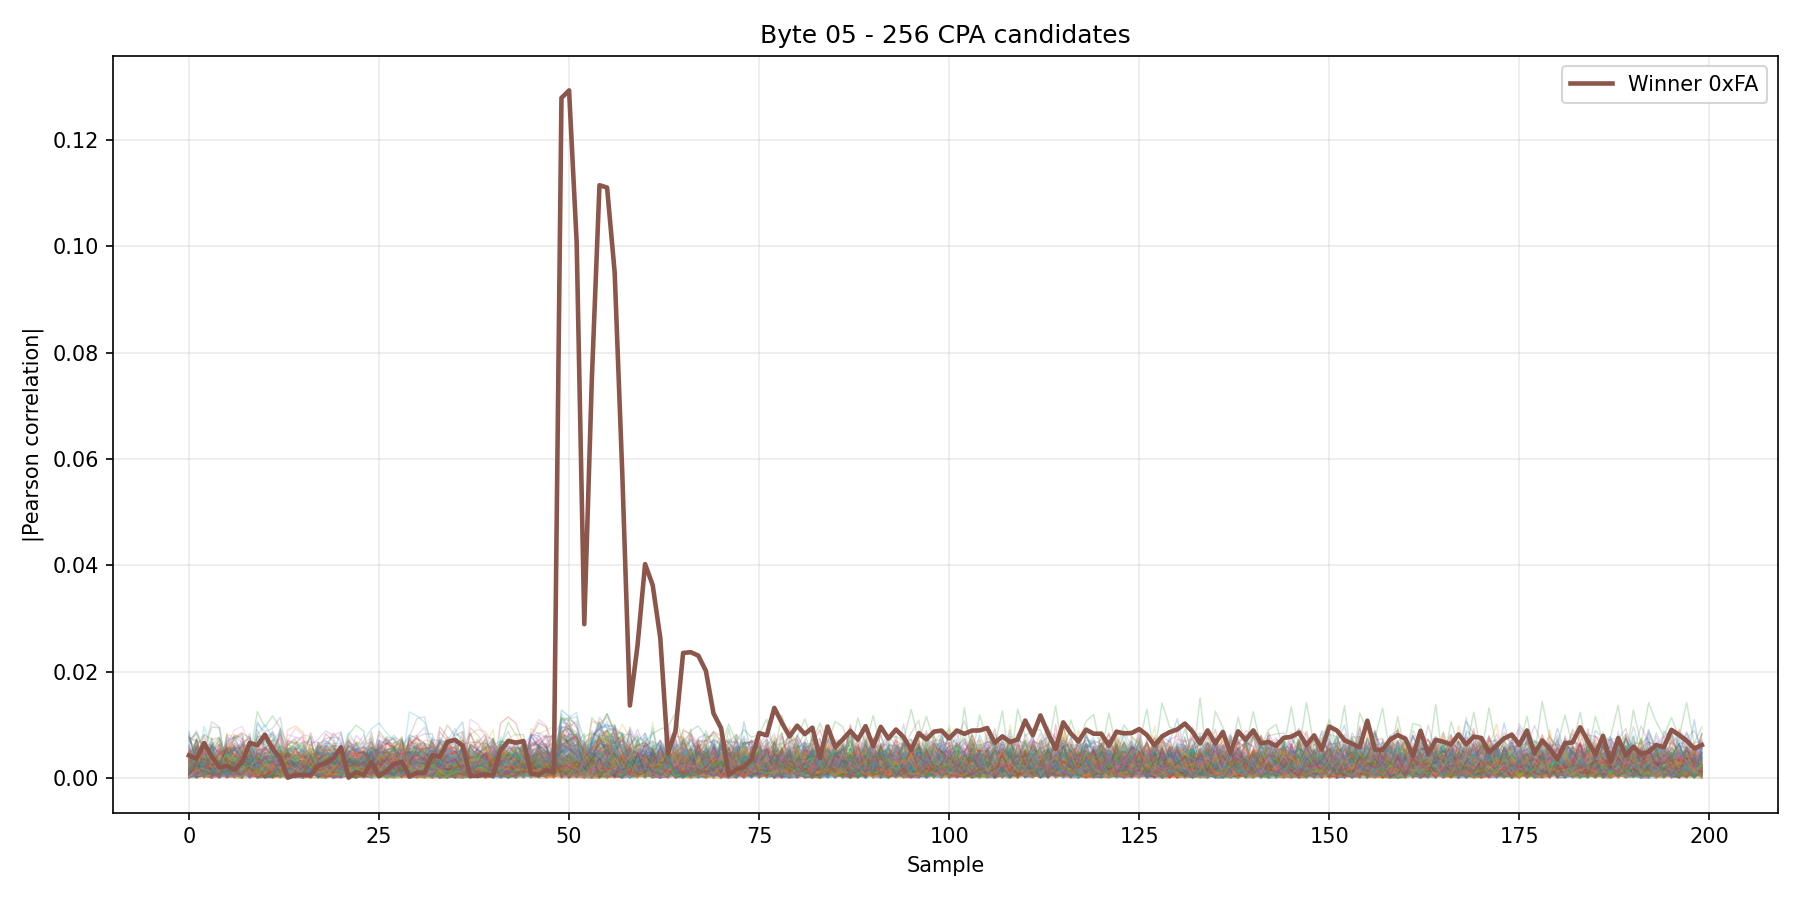
\includegraphics[width=0.92\textwidth]{correlation_plots_full/byte_05.png}
\caption{Task 1: absolute CPA correlations for all 256 candidates at byte 05. The thick curve marks the winning candidate.}
\label{fig:task1-byte-05}
\end{figure}

\begin{figure}[H]
\centering
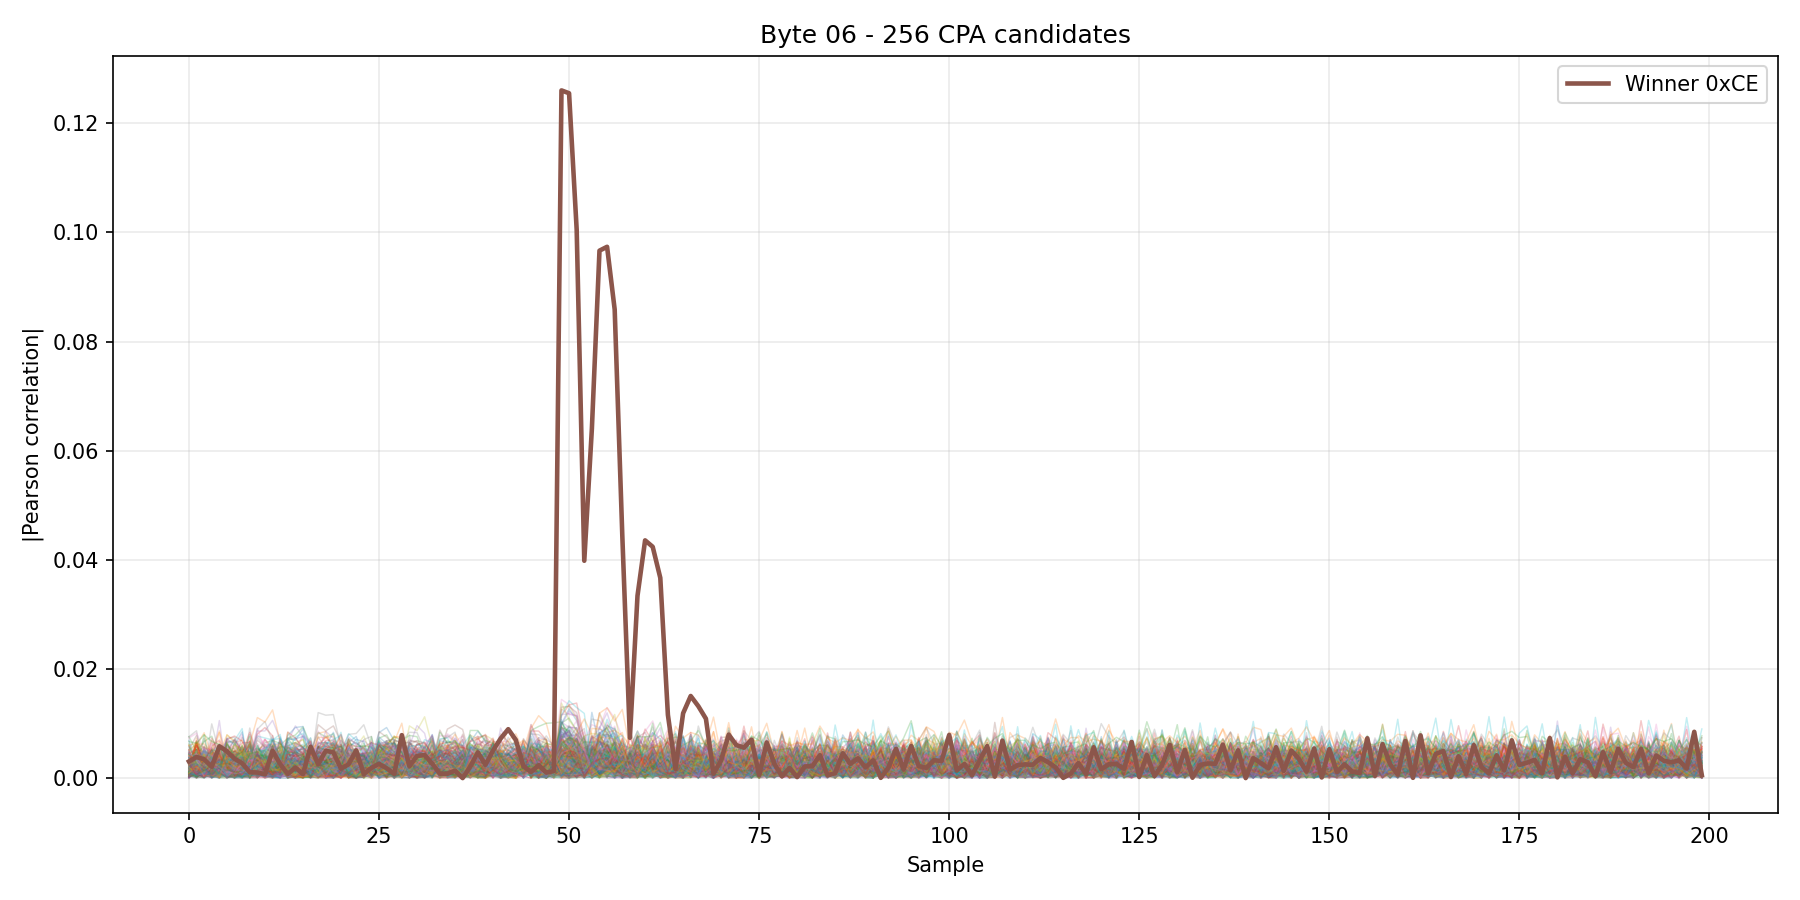
\includegraphics[width=0.92\textwidth]{correlation_plots_full/byte_06.png}
\caption{Task 1: absolute CPA correlations for all 256 candidates at byte 06. The thick curve marks the winning candidate.}
\label{fig:task1-byte-06}
\end{figure}

\clearpage

\begin{figure}[H]
\centering
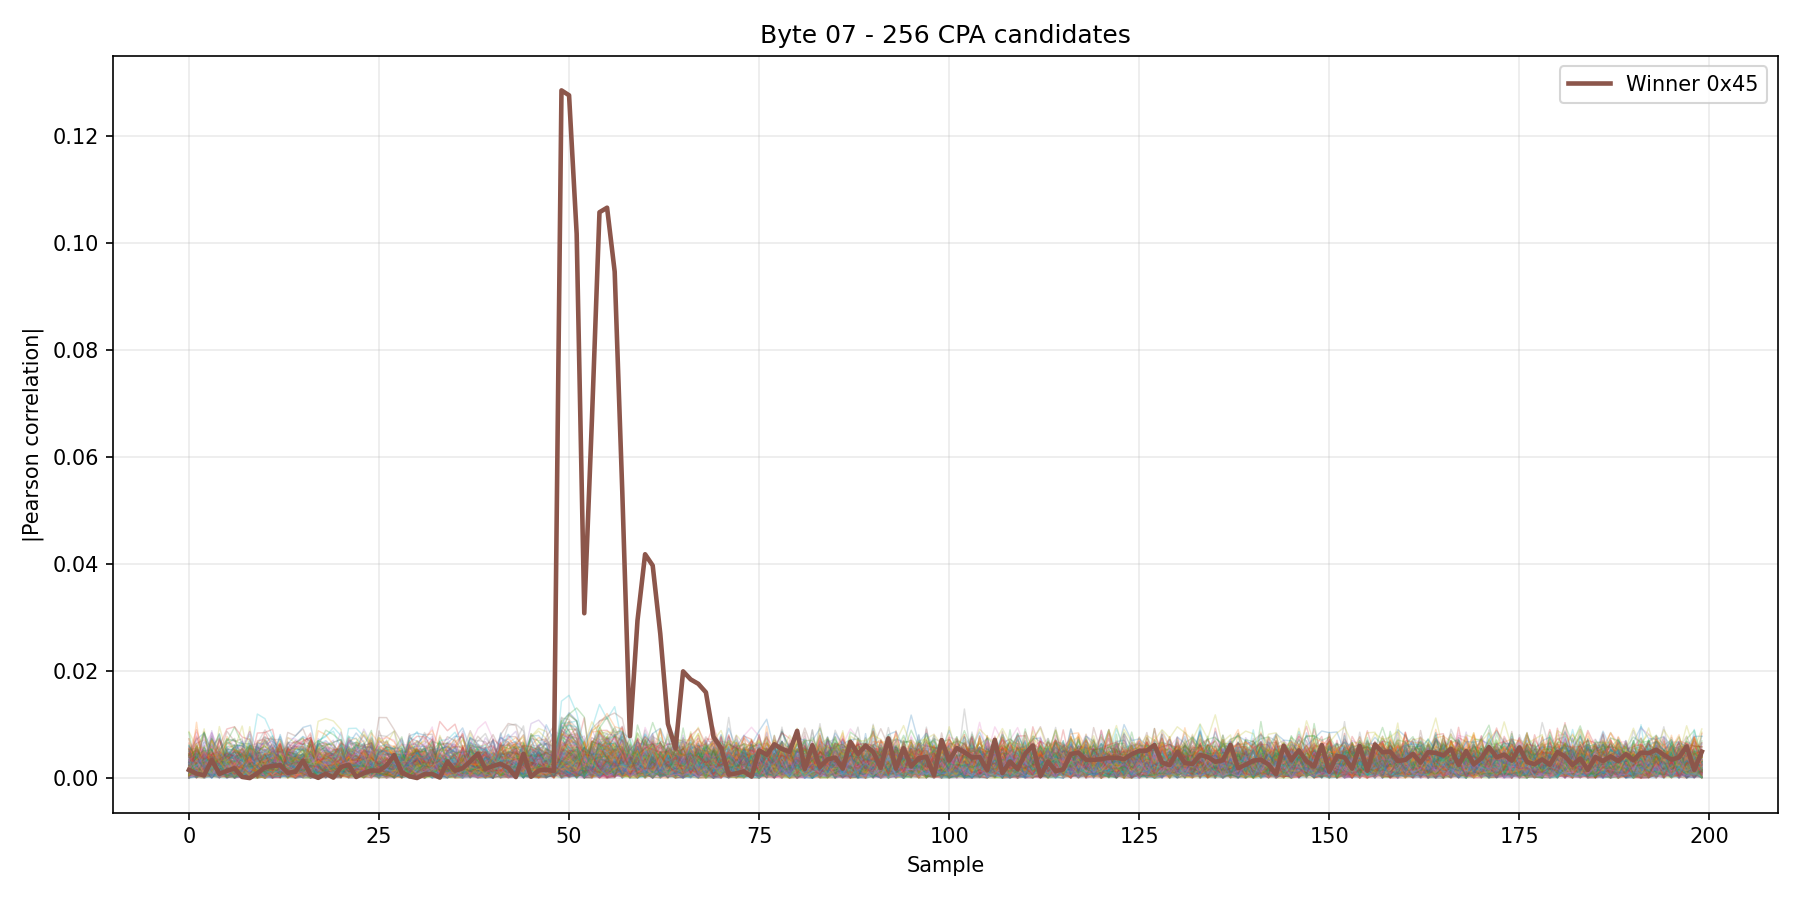
\includegraphics[width=0.92\textwidth]{correlation_plots_full/byte_07.png}
\caption{Task 1: absolute CPA correlations for all 256 candidates at byte 07. The thick curve marks the winning candidate.}
\label{fig:task1-byte-07}
\end{figure}

\begin{figure}[H]
\centering
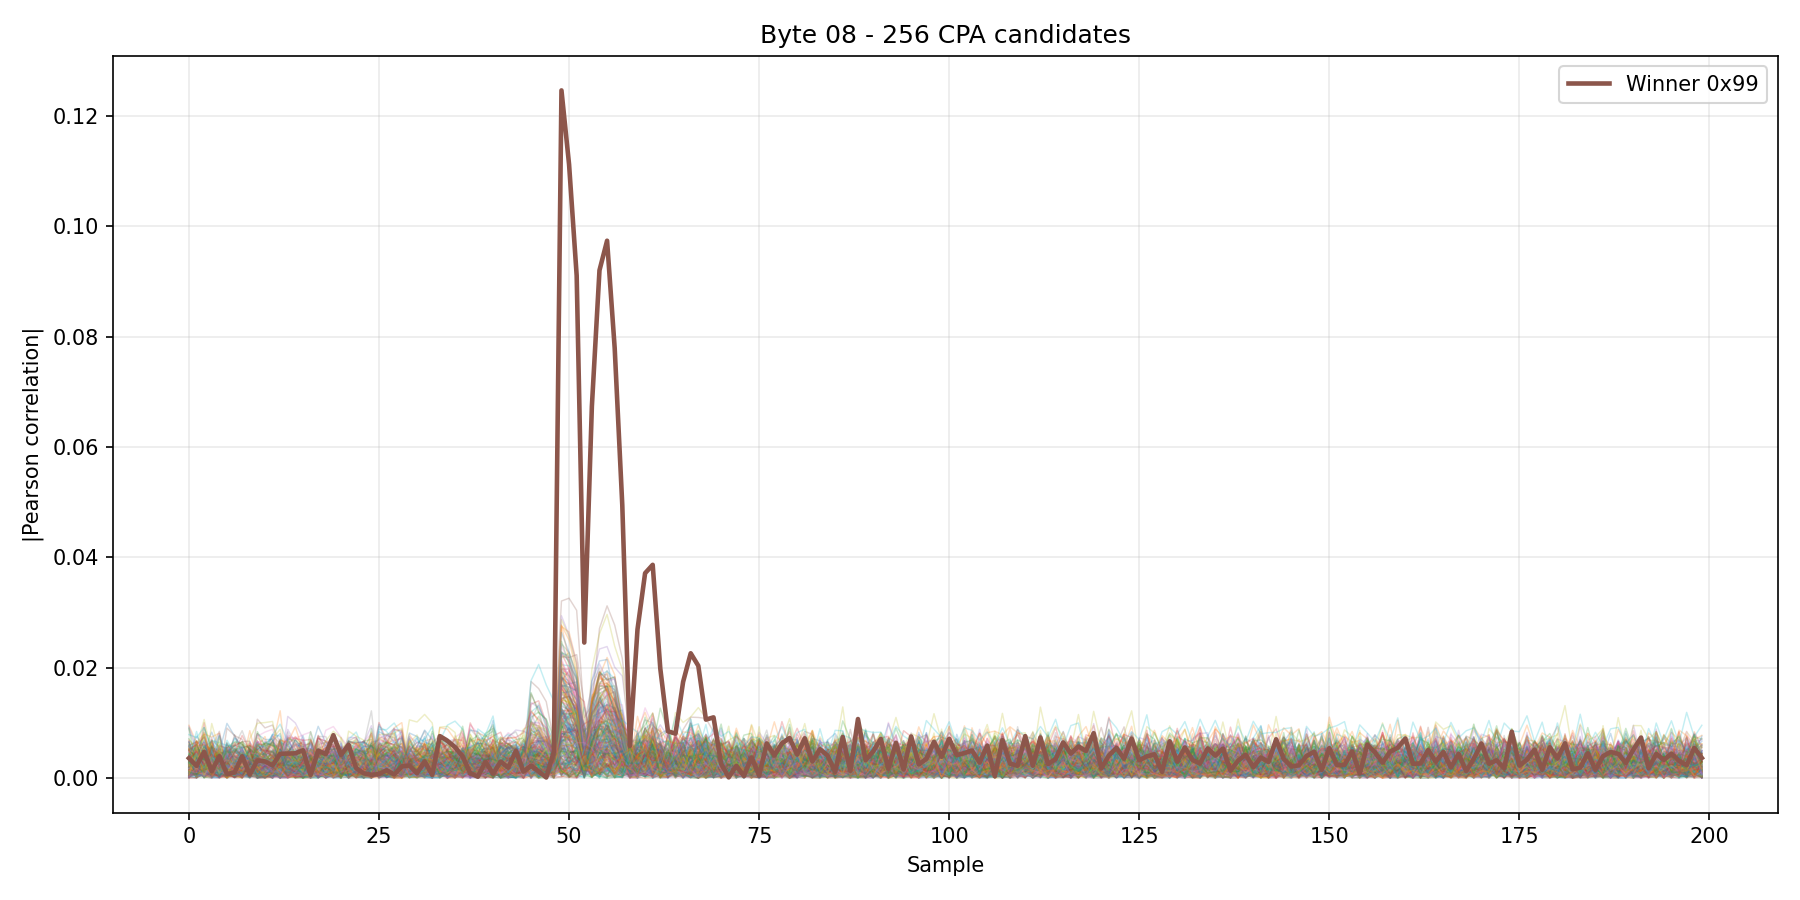
\includegraphics[width=0.92\textwidth]{correlation_plots_full/byte_08.png}
\caption{Task 1: absolute CPA correlations for all 256 candidates at byte 08. The thick curve marks the winning candidate.}
\label{fig:task1-byte-08}
\end{figure}

\clearpage

\begin{figure}[H]
\centering
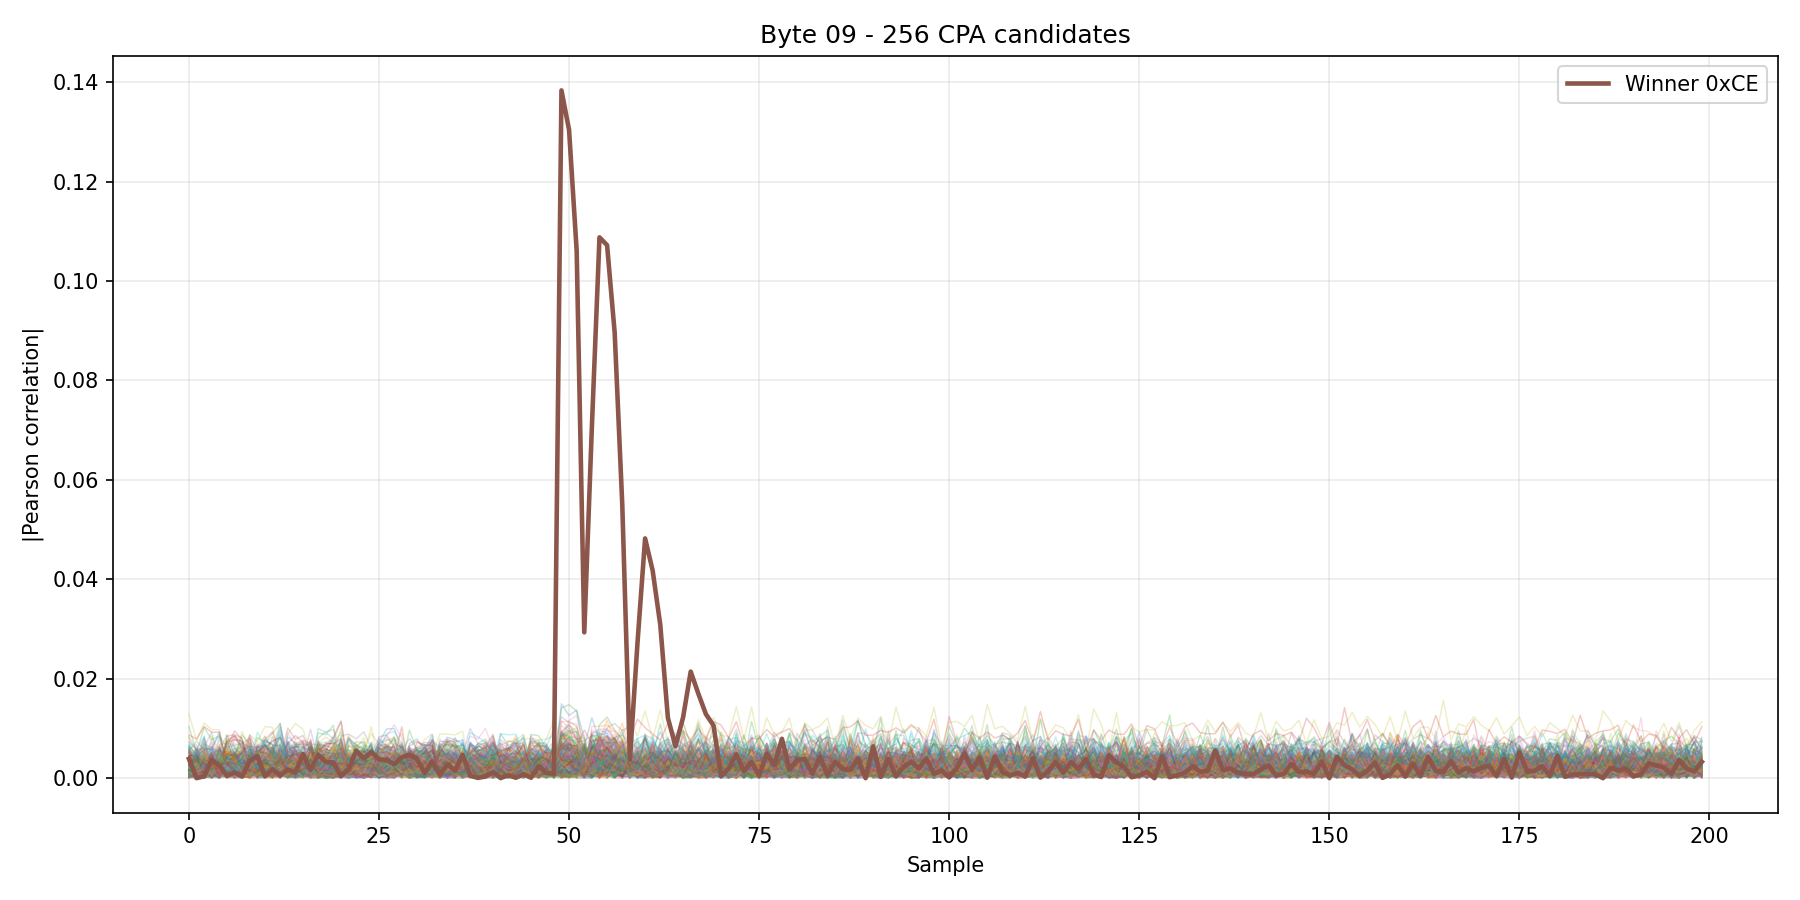
\includegraphics[width=0.92\textwidth]{correlation_plots_full/byte_09.png}
\caption{Task 1: absolute CPA correlations for all 256 candidates at byte 09. The thick curve marks the winning candidate.}
\label{fig:task1-byte-09}
\end{figure}

\begin{figure}[H]
\centering
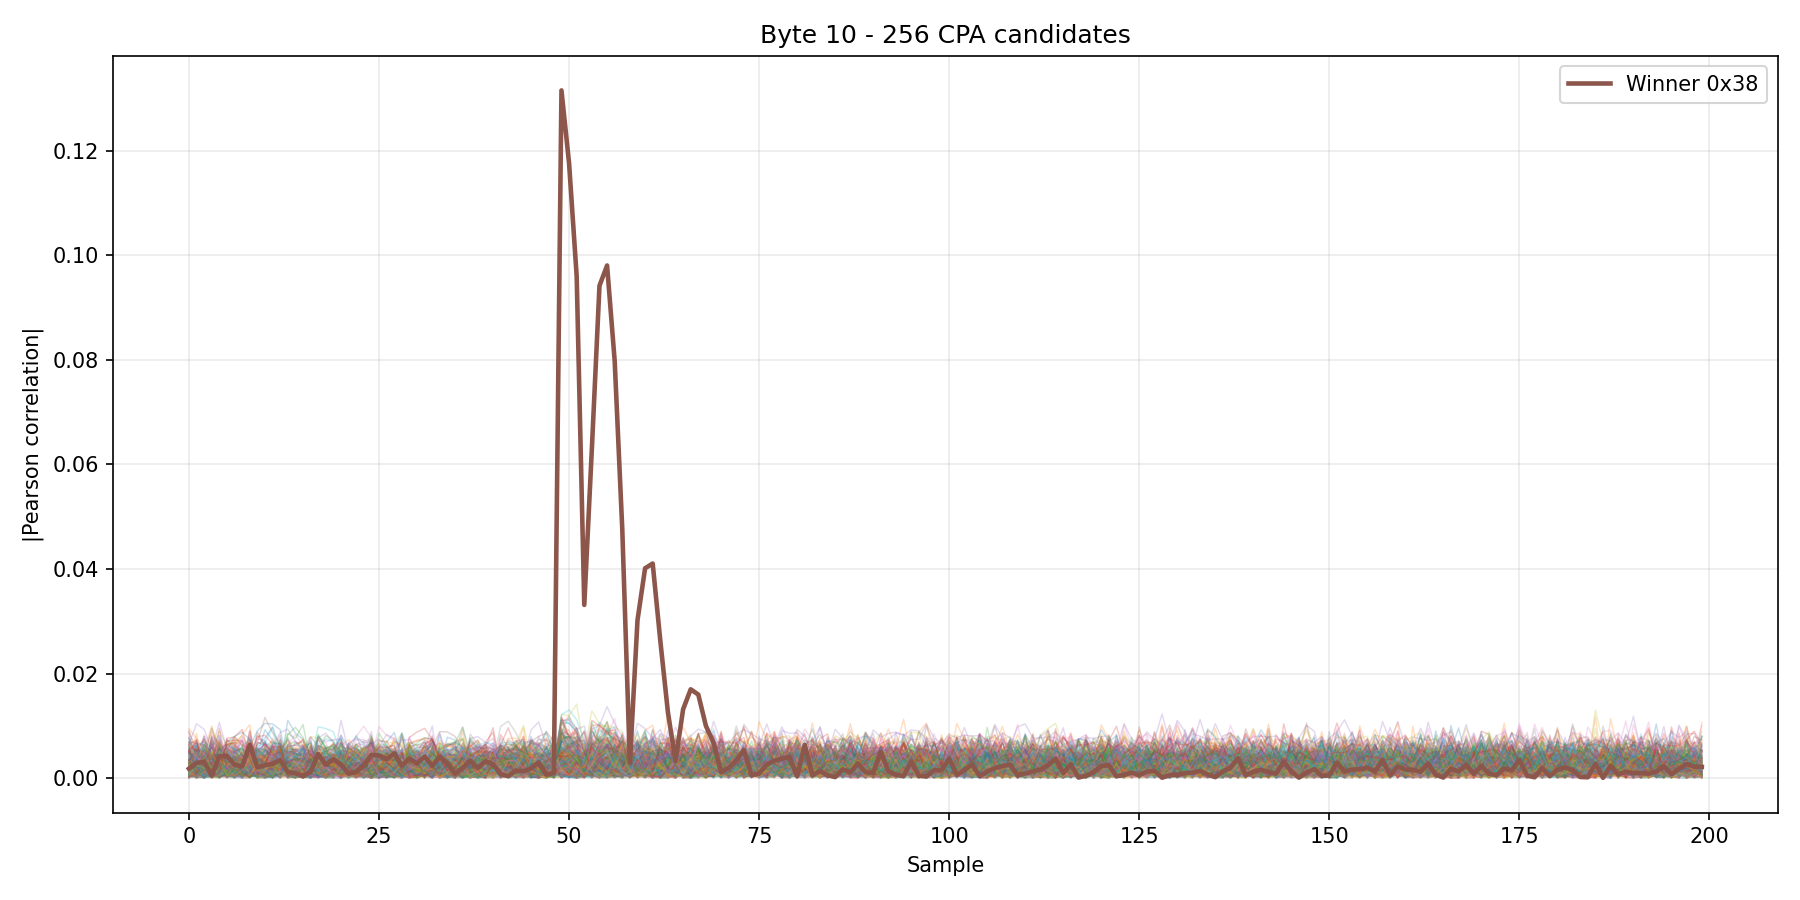
\includegraphics[width=0.92\textwidth]{correlation_plots_full/byte_10.png}
\caption{Task 1: absolute CPA correlations for all 256 candidates at byte 10. The thick curve marks the winning candidate.}
\label{fig:task1-byte-10}
\end{figure}

\clearpage

\begin{figure}[H]
\centering
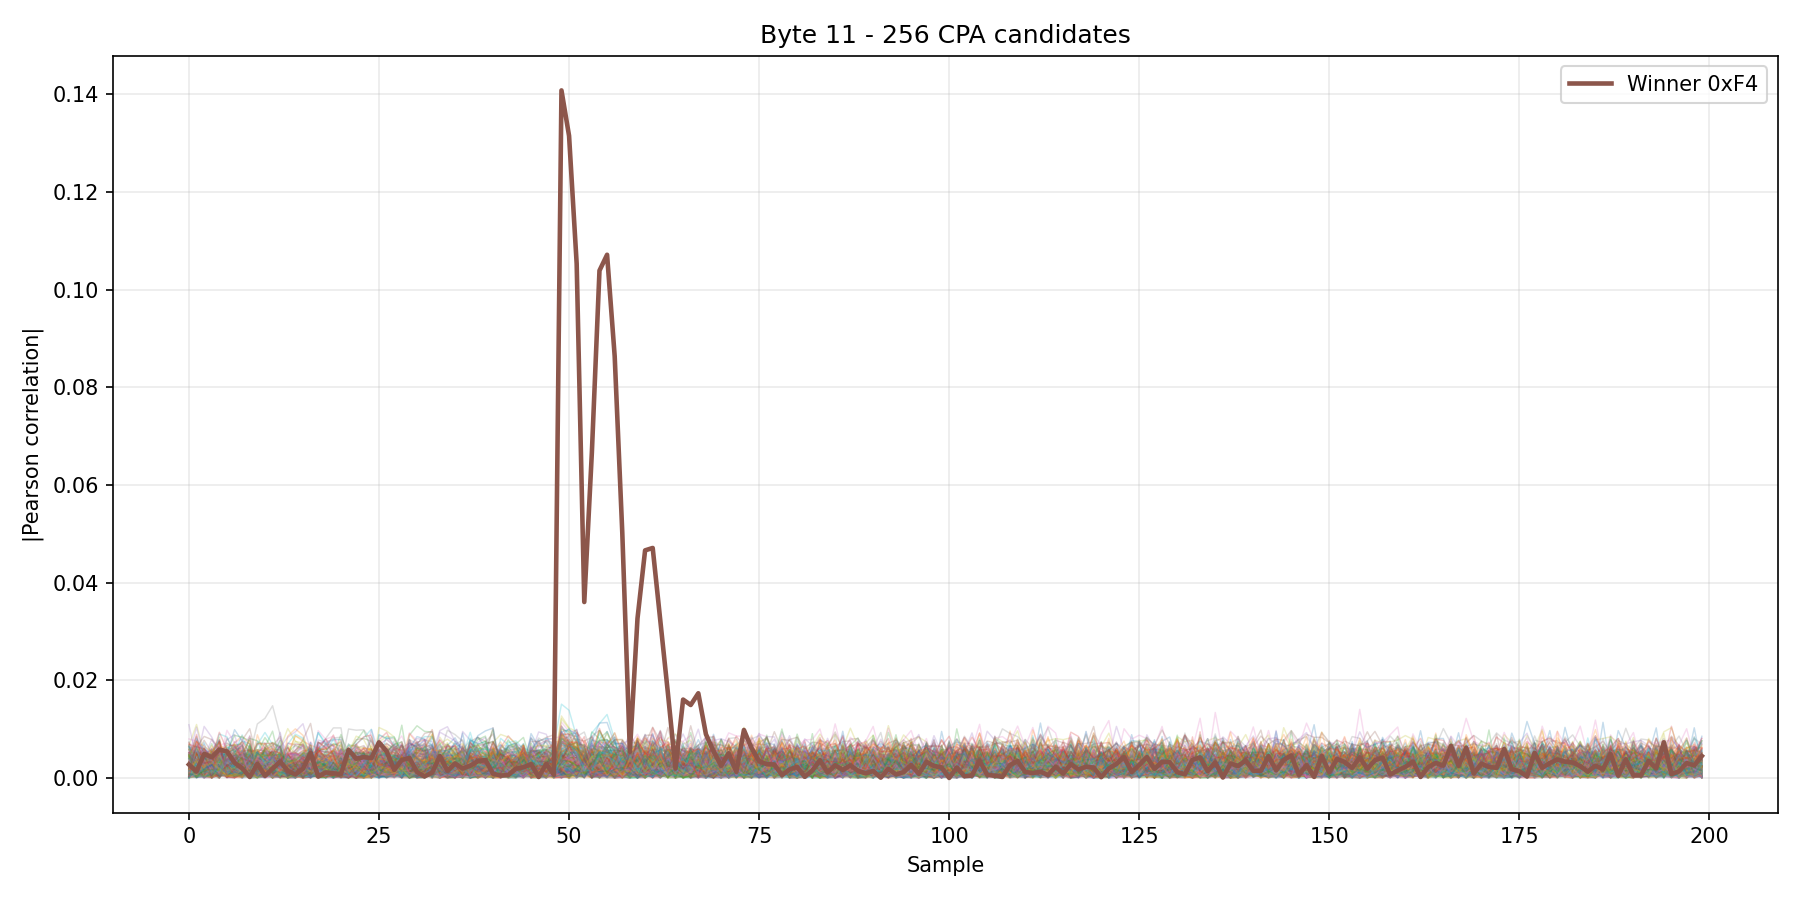
\includegraphics[width=0.92\textwidth]{correlation_plots_full/byte_11.png}
\caption{Task 1: absolute CPA correlations for all 256 candidates at byte 11. The thick curve marks the winning candidate.}
\label{fig:task1-byte-11}
\end{figure}

\begin{figure}[H]
\centering
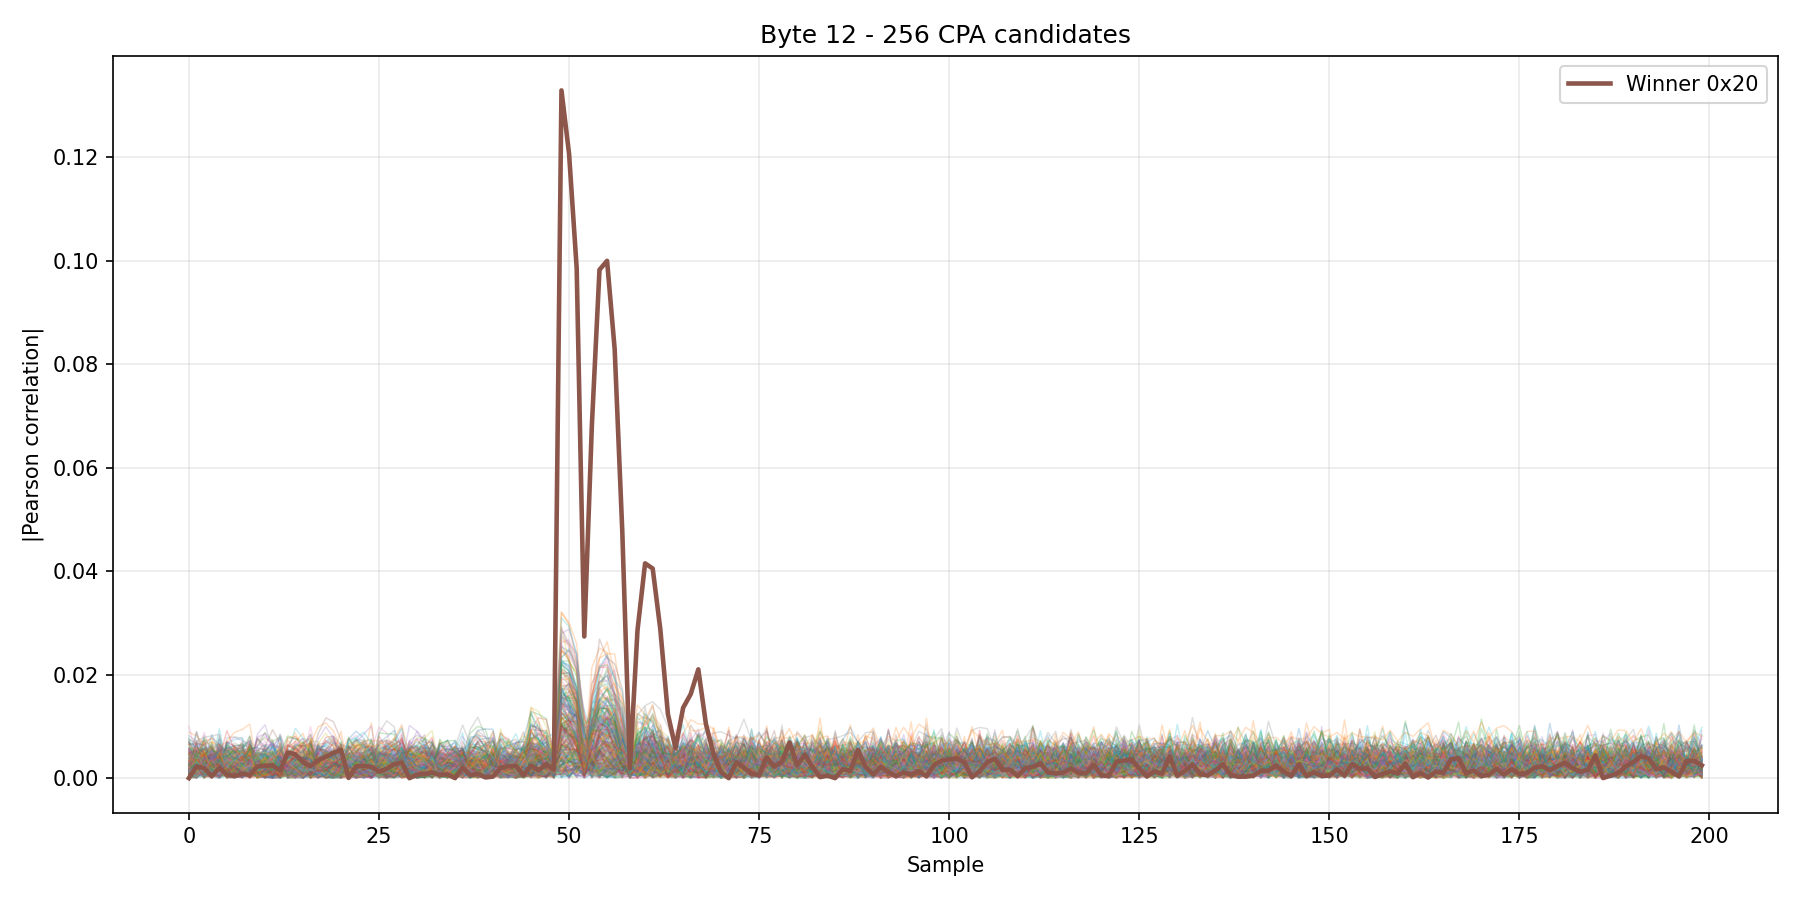
\includegraphics[width=0.92\textwidth]{correlation_plots_full/byte_12.png}
\caption{Task 1: absolute CPA correlations for all 256 candidates at byte 12. The thick curve marks the winning candidate.}
\label{fig:task1-byte-12}
\end{figure}

\clearpage

\begin{figure}[H]
\centering
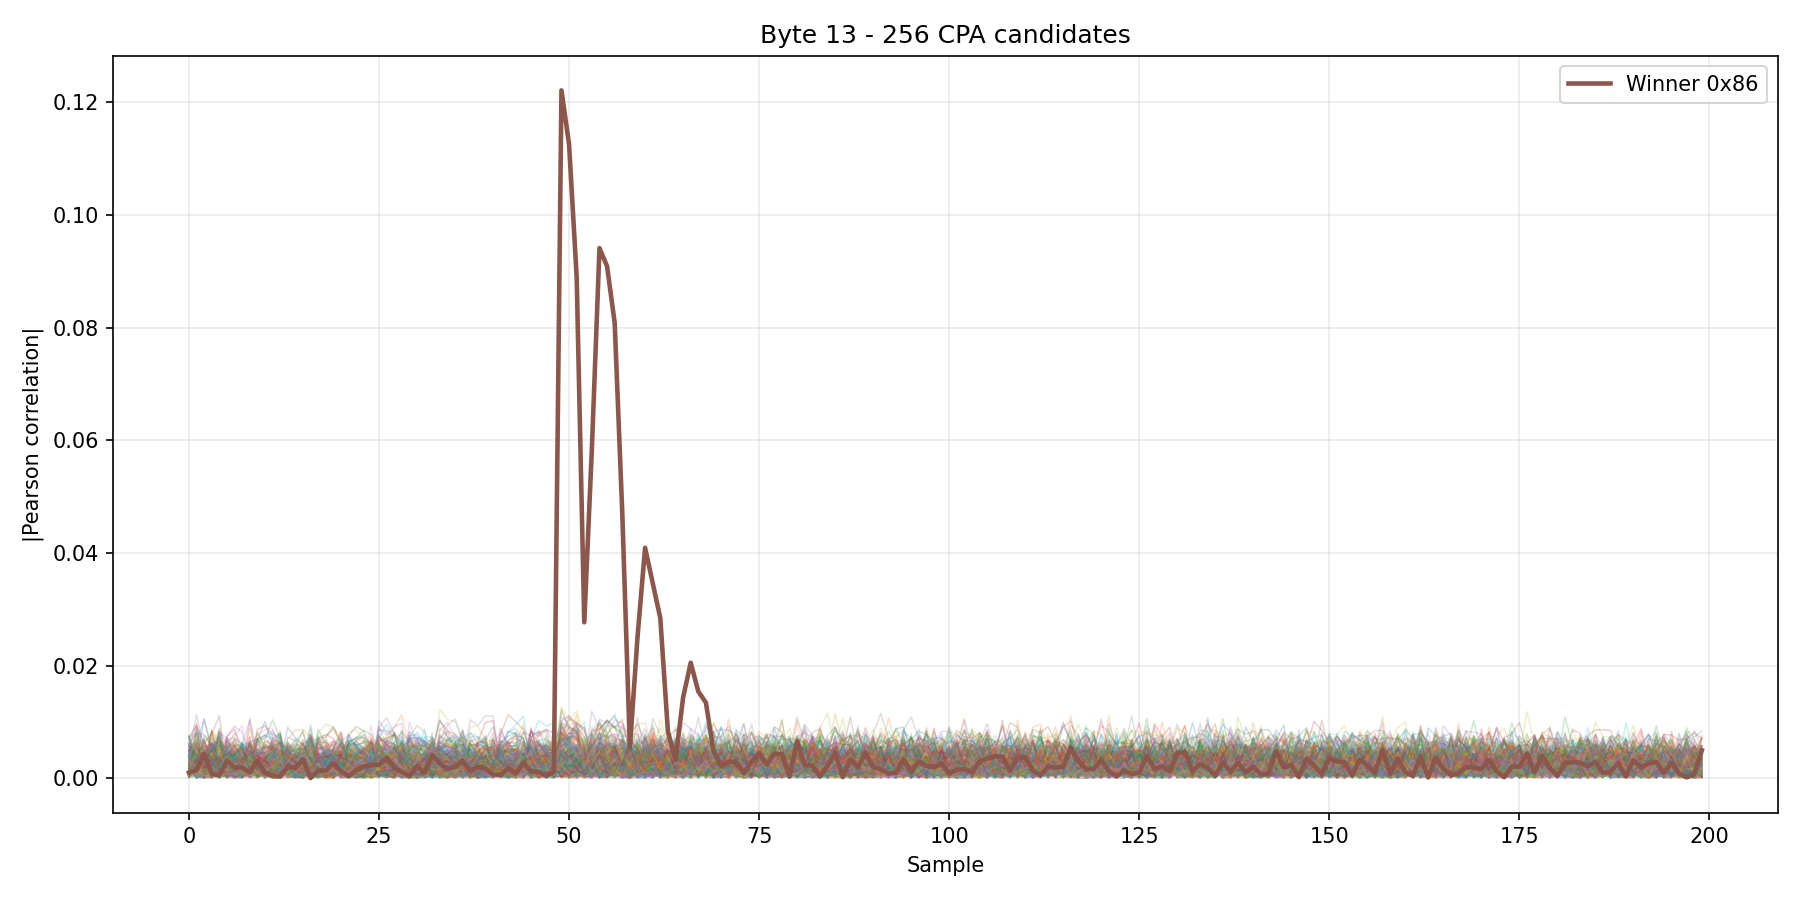
\includegraphics[width=0.92\textwidth]{correlation_plots_full/byte_13.png}
\caption{Task 1: absolute CPA correlations for all 256 candidates at byte 13. The thick curve marks the winning candidate.}
\label{fig:task1-byte-13}
\end{figure}

\begin{figure}[H]
\centering
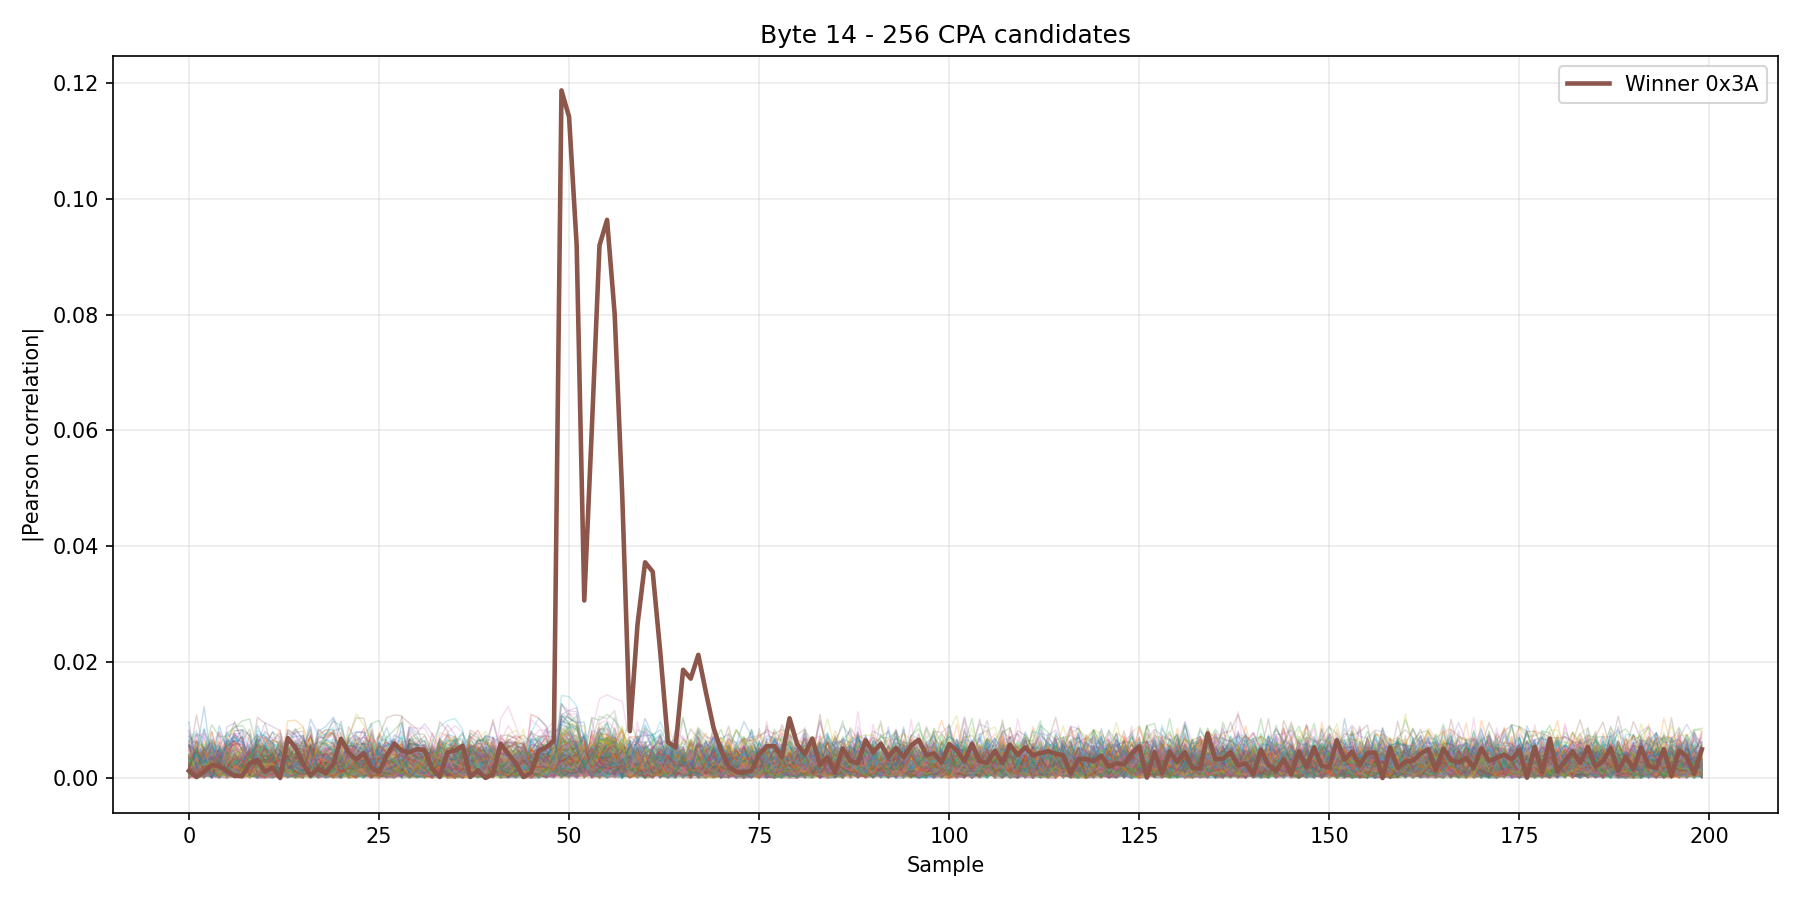
\includegraphics[width=0.92\textwidth]{correlation_plots_full/byte_14.png}
\caption{Task 1: absolute CPA correlations for all 256 candidates at byte 14. The thick curve marks the winning candidate.}
\label{fig:task1-byte-14}
\end{figure}

\clearpage

\begin{figure}[H]
\centering
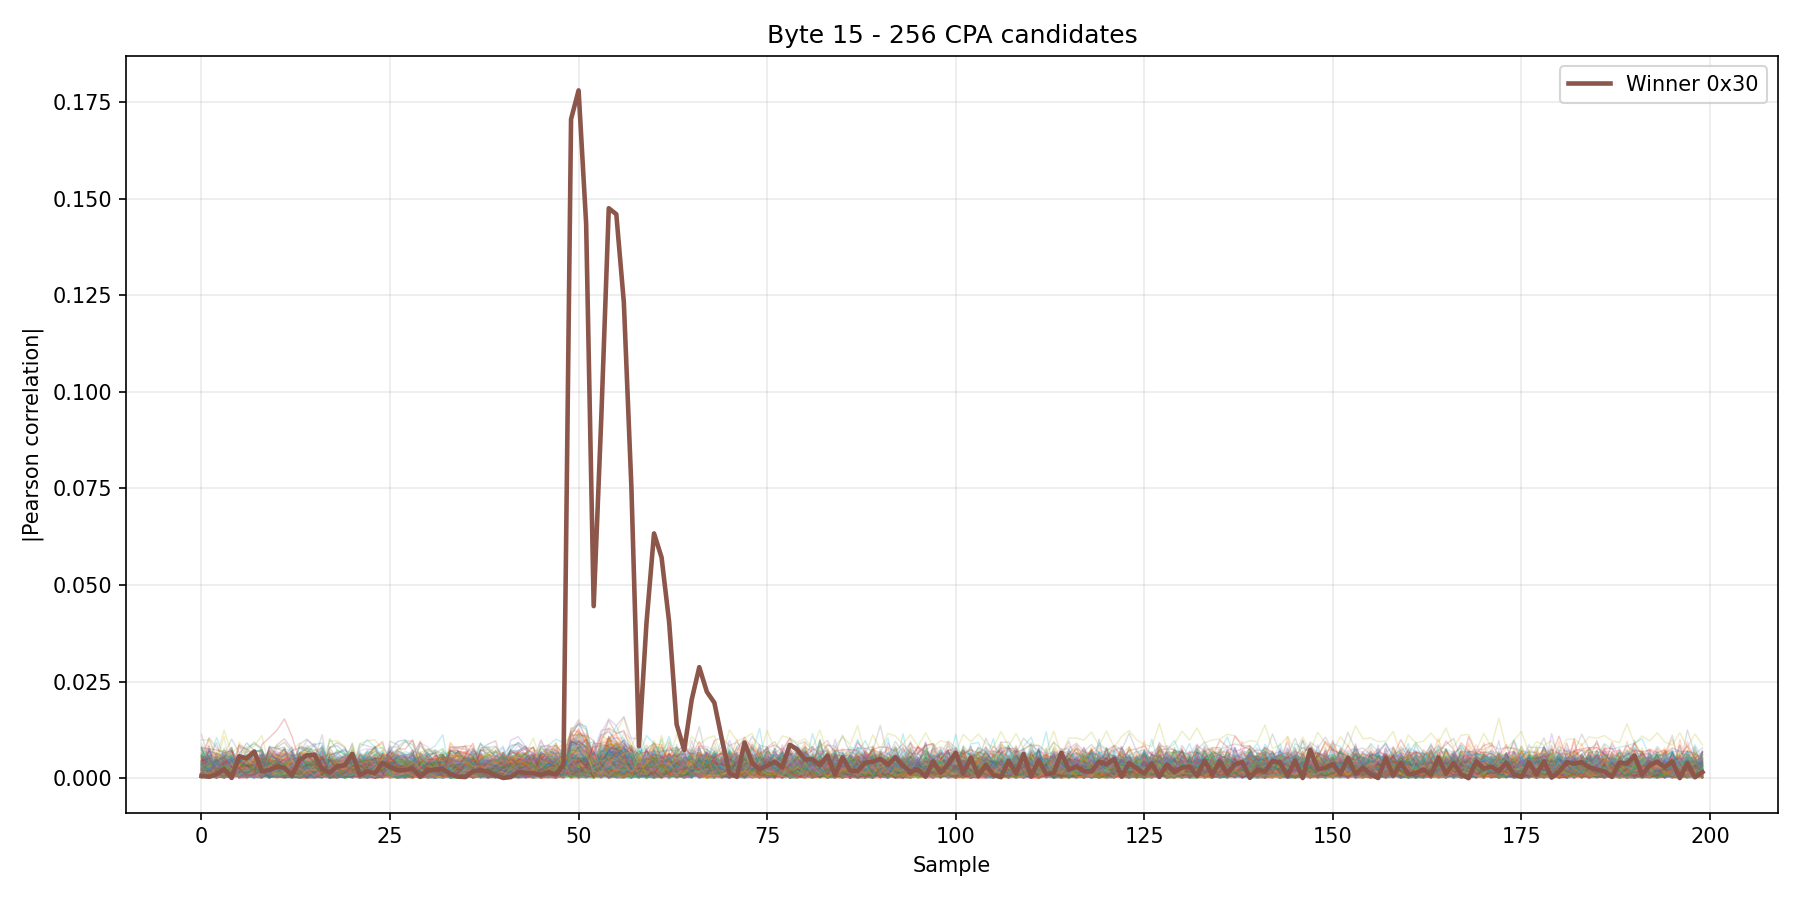
\includegraphics[width=0.92\textwidth]{correlation_plots_full/byte_15.png}
\caption{Task 1: absolute CPA correlations for all 256 candidates at byte 15. The thick curve marks the winning candidate.}
\label{fig:task1-byte-15}
\end{figure}

\clearpage

\section{Actual round-10 key correlation plots}
\label{app:task3-plots}
Figure~\ref{fig:task3-example} shows byte 0. The following plots cover bytes 1 through 15.

\begin{figure}[H]
\centering
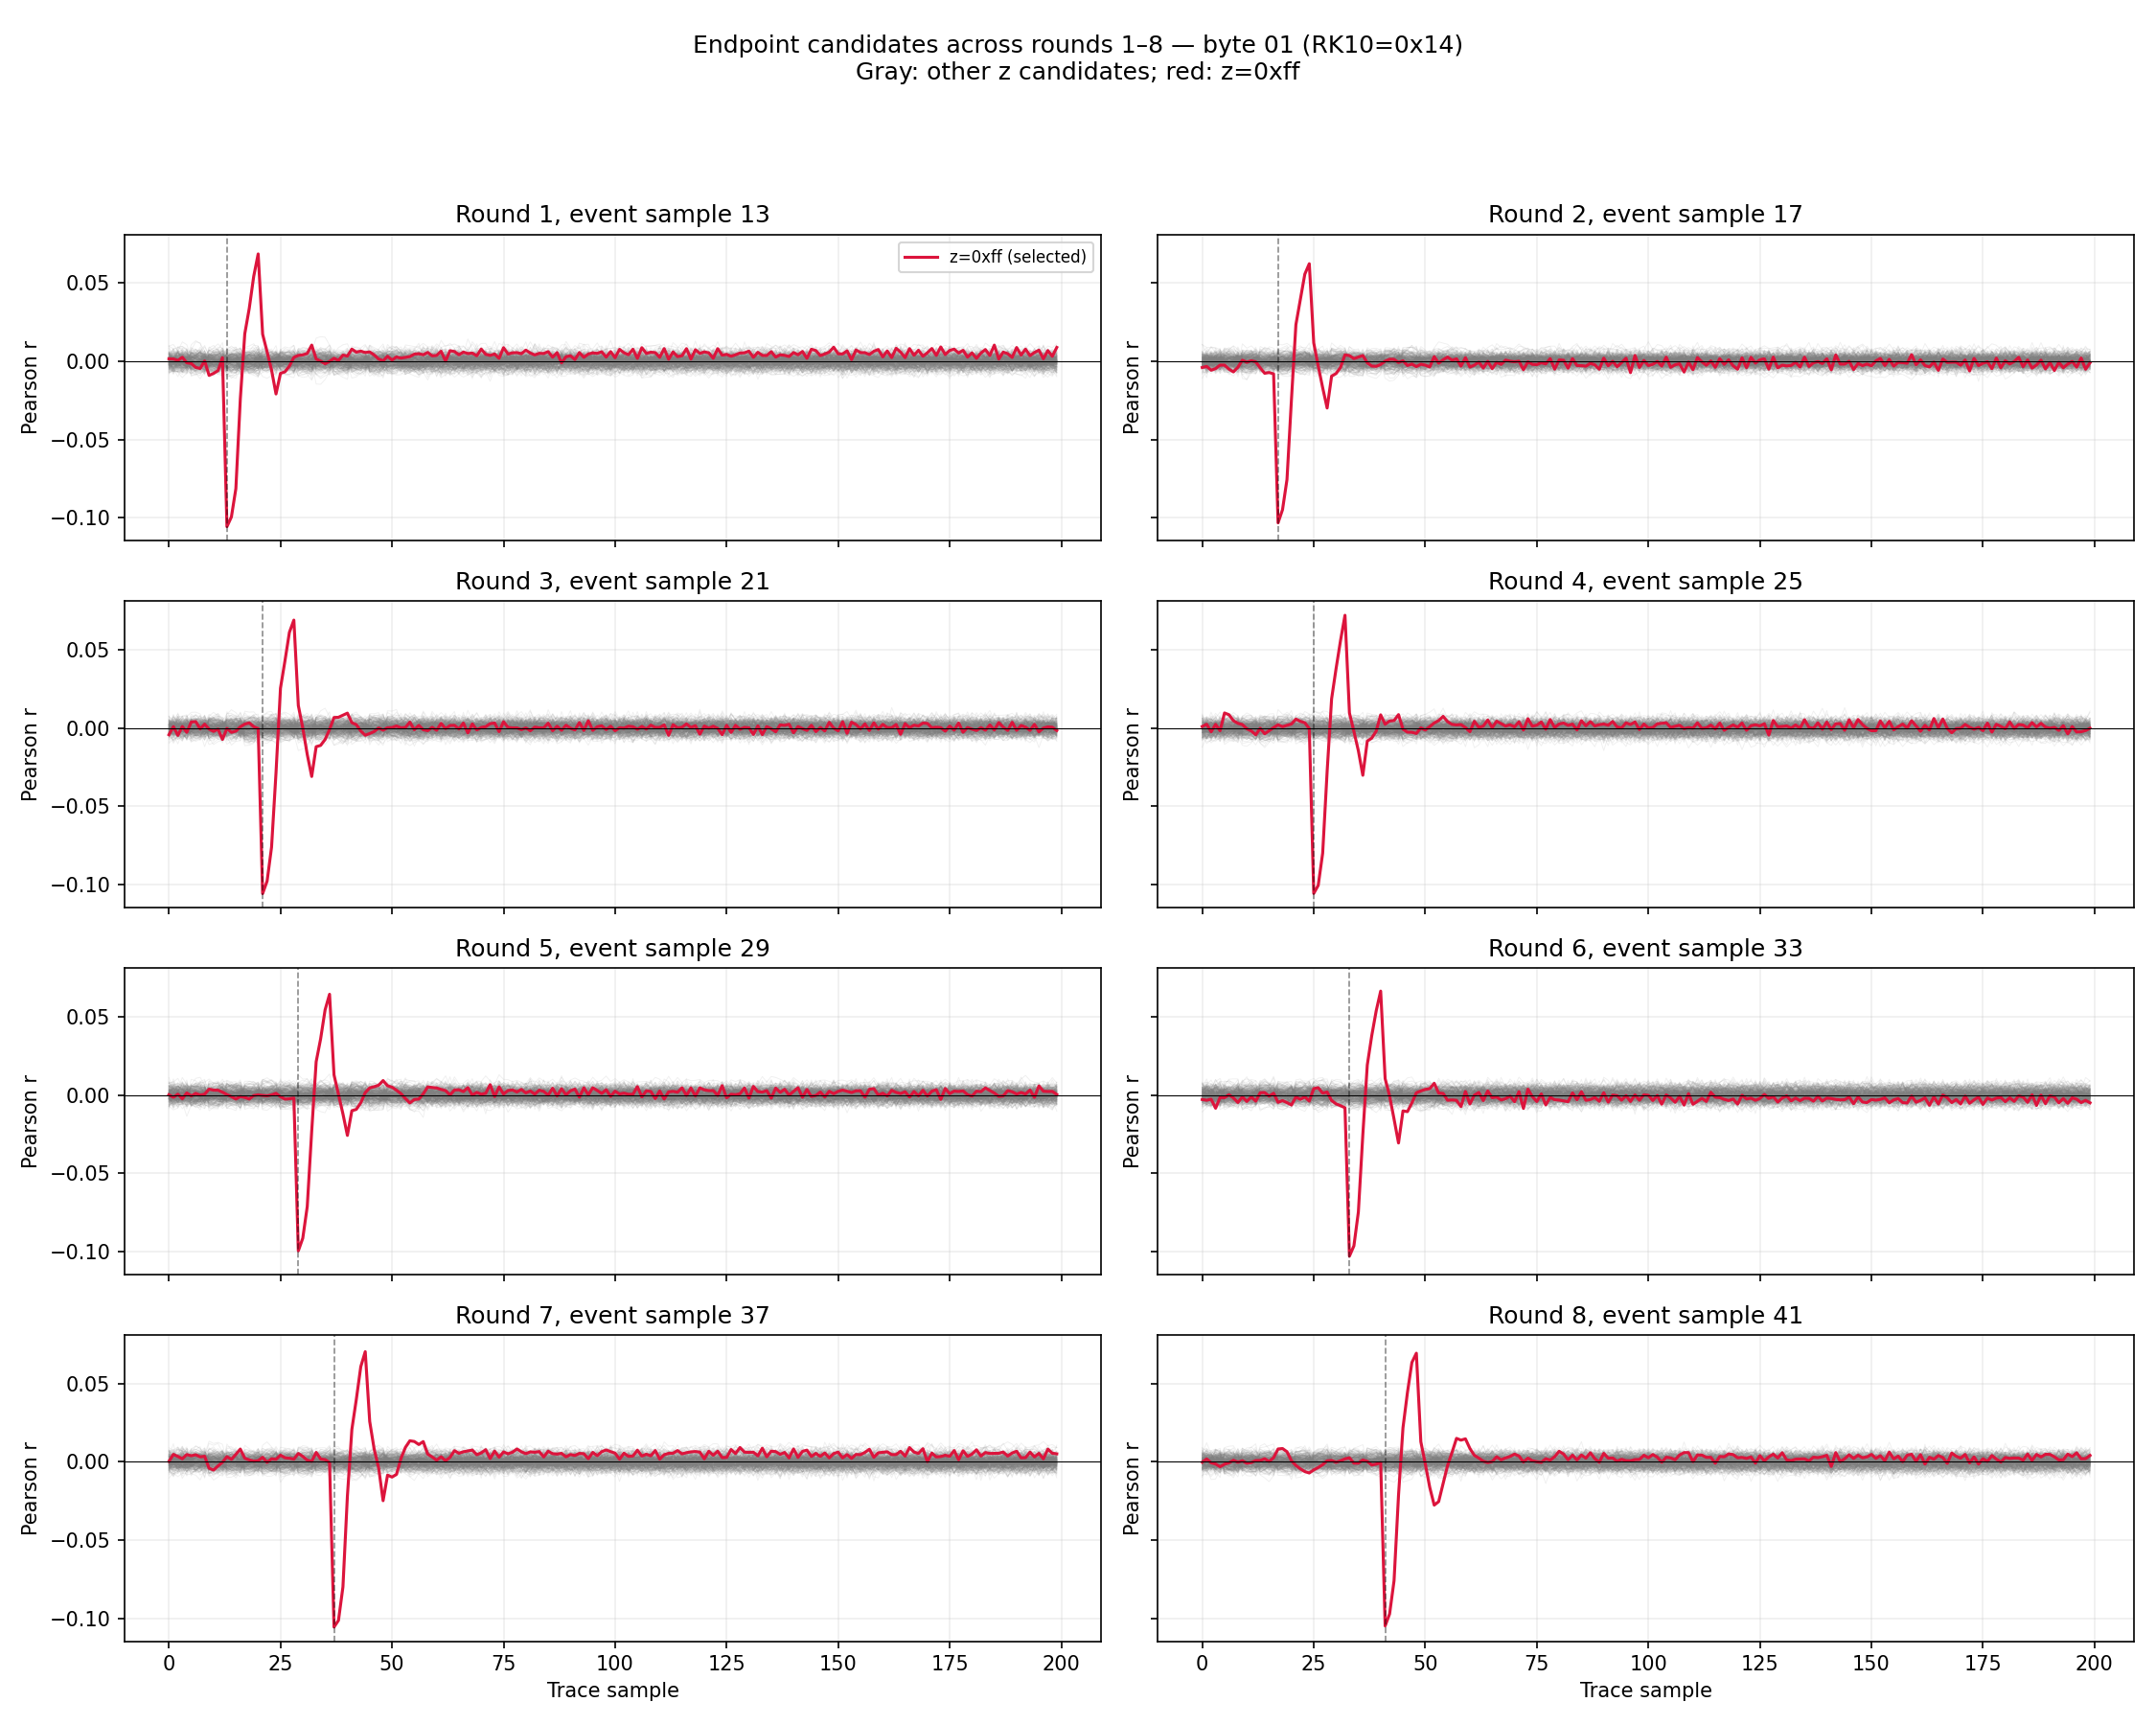
\includegraphics[width=0.96\textwidth]{actual_round10_correlation_plots/byte_01.png}
\caption{Task 3: endpoint-candidate correlations for byte 01 across rounds 1--8. Red curves mark the selected $z=\texttt{0xFF}$; dashed lines mark the detected event samples.}
\label{fig:task3-byte-01}
\end{figure}

\clearpage

\begin{figure}[H]
\centering
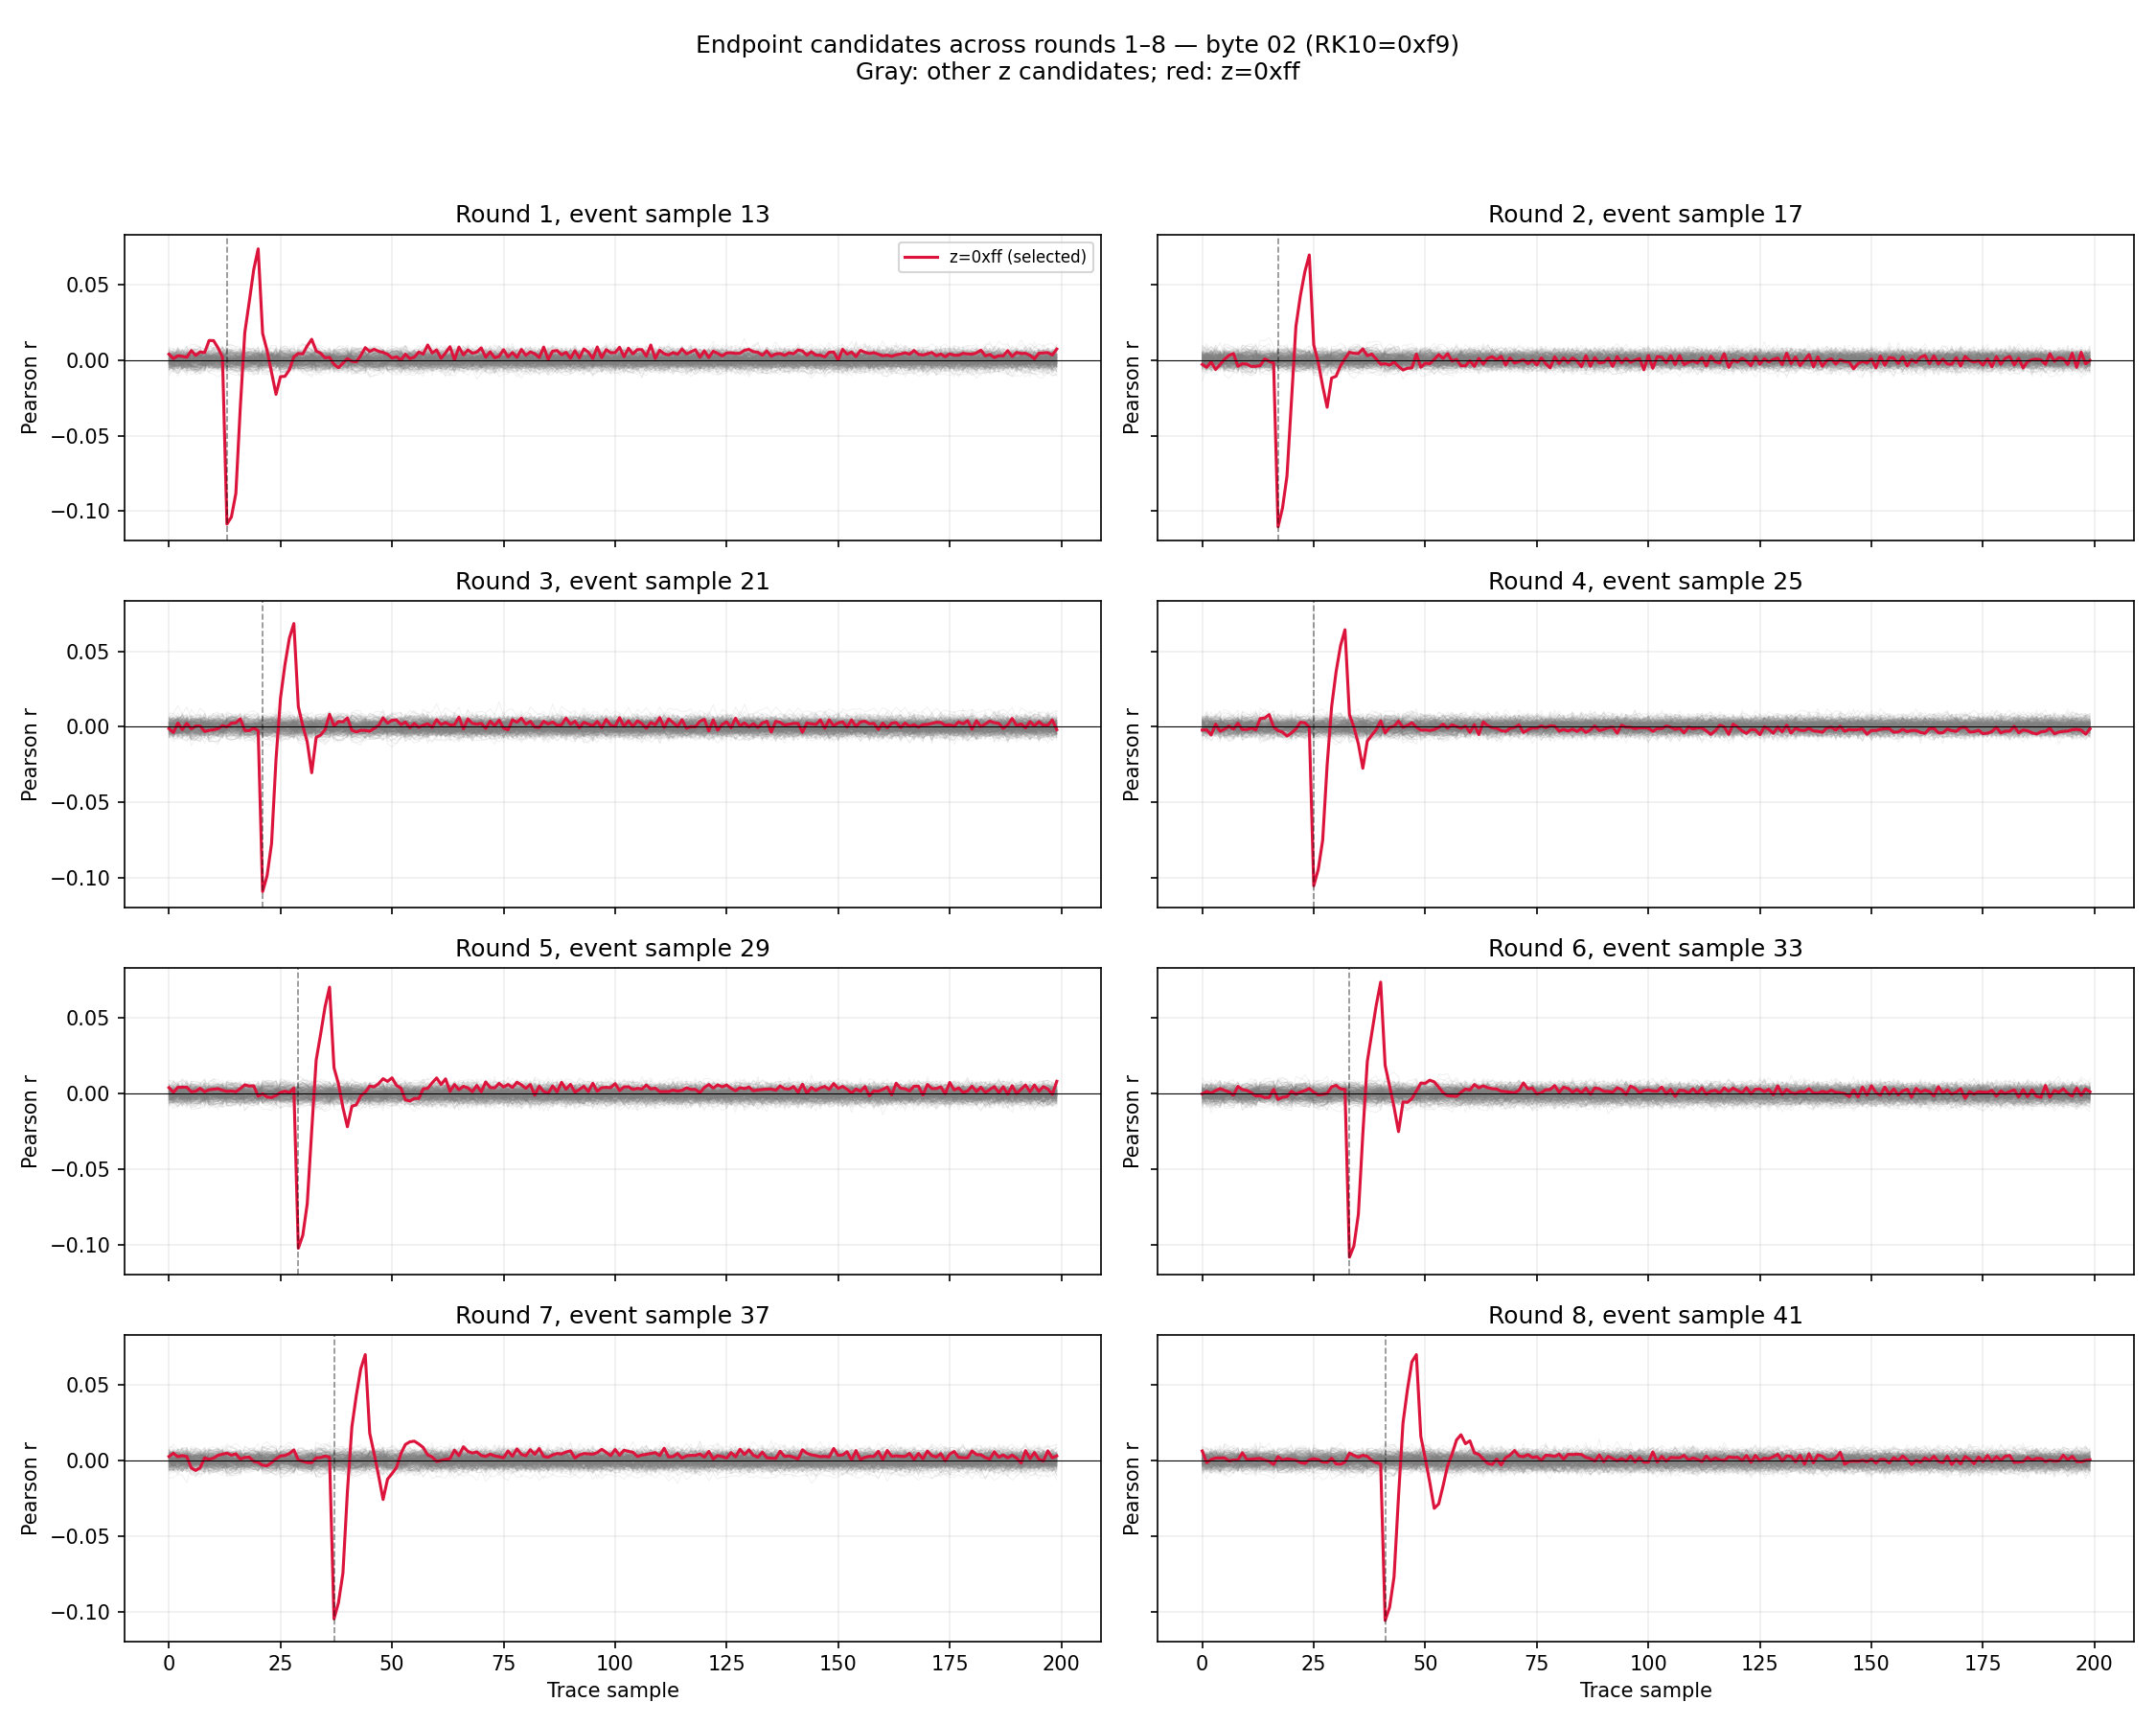
\includegraphics[width=0.96\textwidth]{actual_round10_correlation_plots/byte_02.png}
\caption{Task 3: endpoint-candidate correlations for byte 02 across rounds 1--8. Red curves mark the selected $z=\texttt{0xFF}$; dashed lines mark the detected event samples.}
\label{fig:task3-byte-02}
\end{figure}

\clearpage

\begin{figure}[H]
\centering
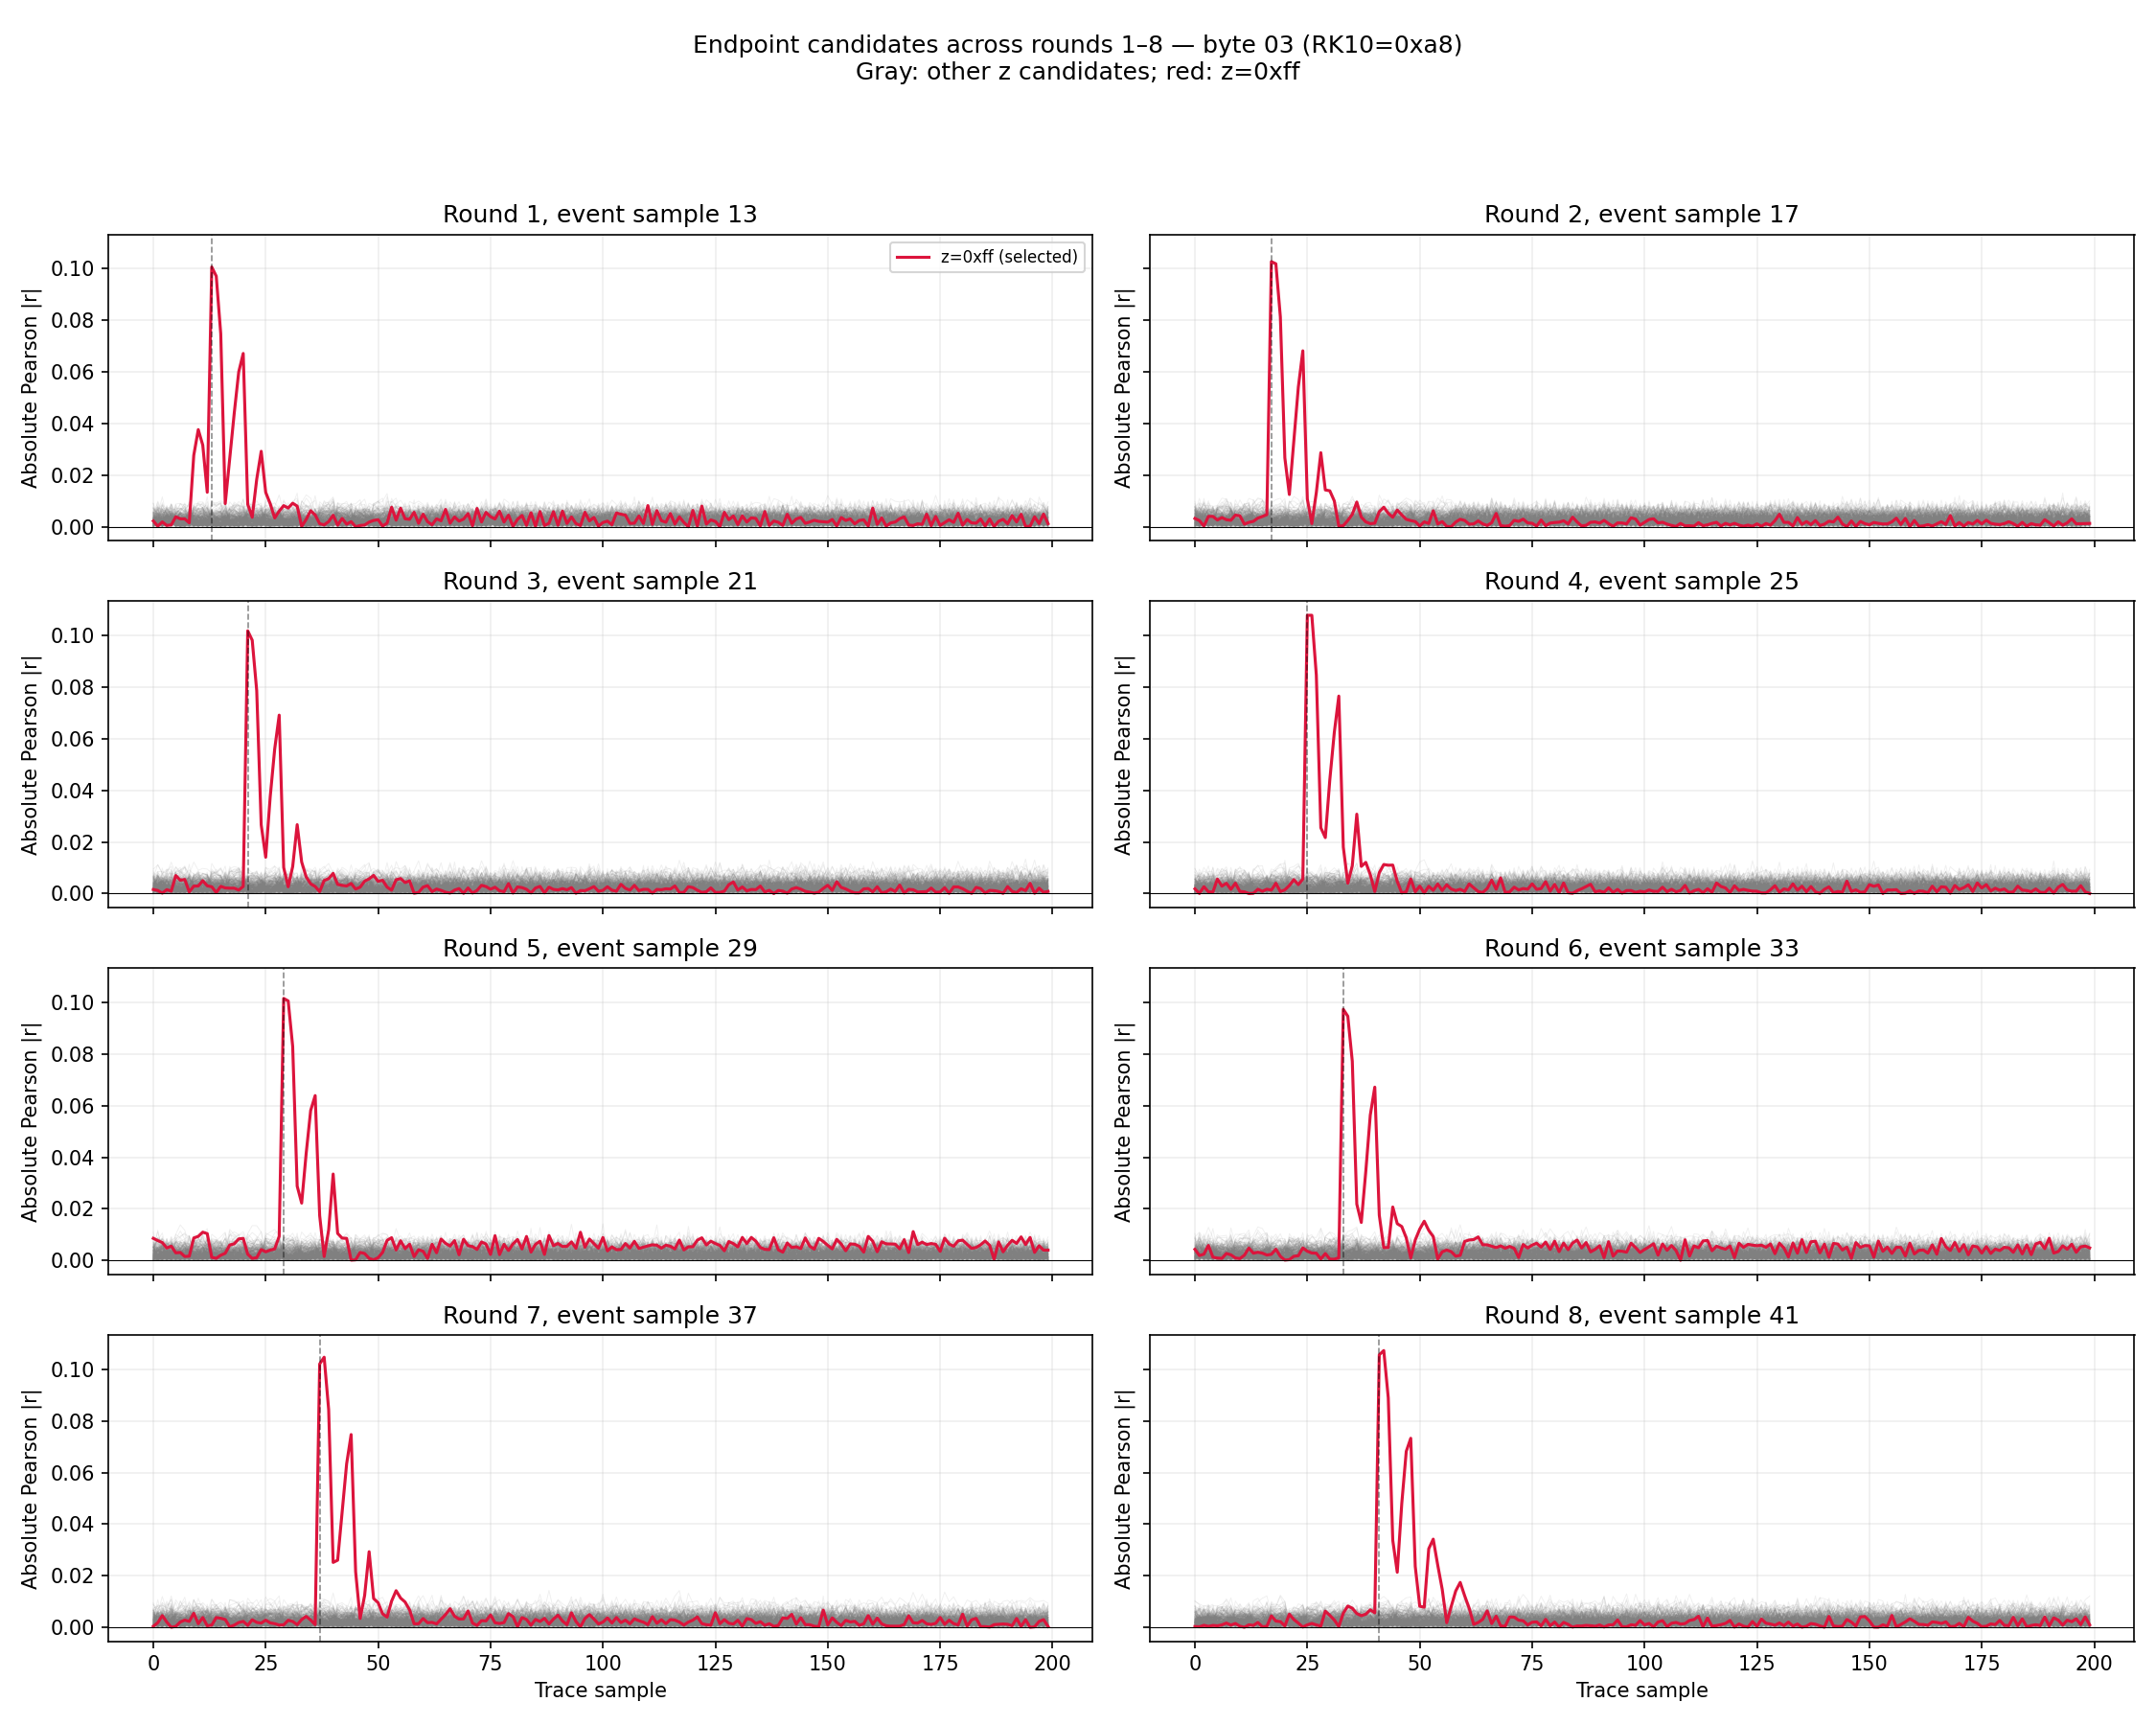
\includegraphics[width=0.96\textwidth]{actual_round10_correlation_plots/byte_03.png}
\caption{Task 3: endpoint-candidate correlations for byte 03 across rounds 1--8. Red curves mark the selected $z=\texttt{0xFF}$; dashed lines mark the detected event samples.}
\label{fig:task3-byte-03}
\end{figure}

\clearpage

\begin{figure}[H]
\centering
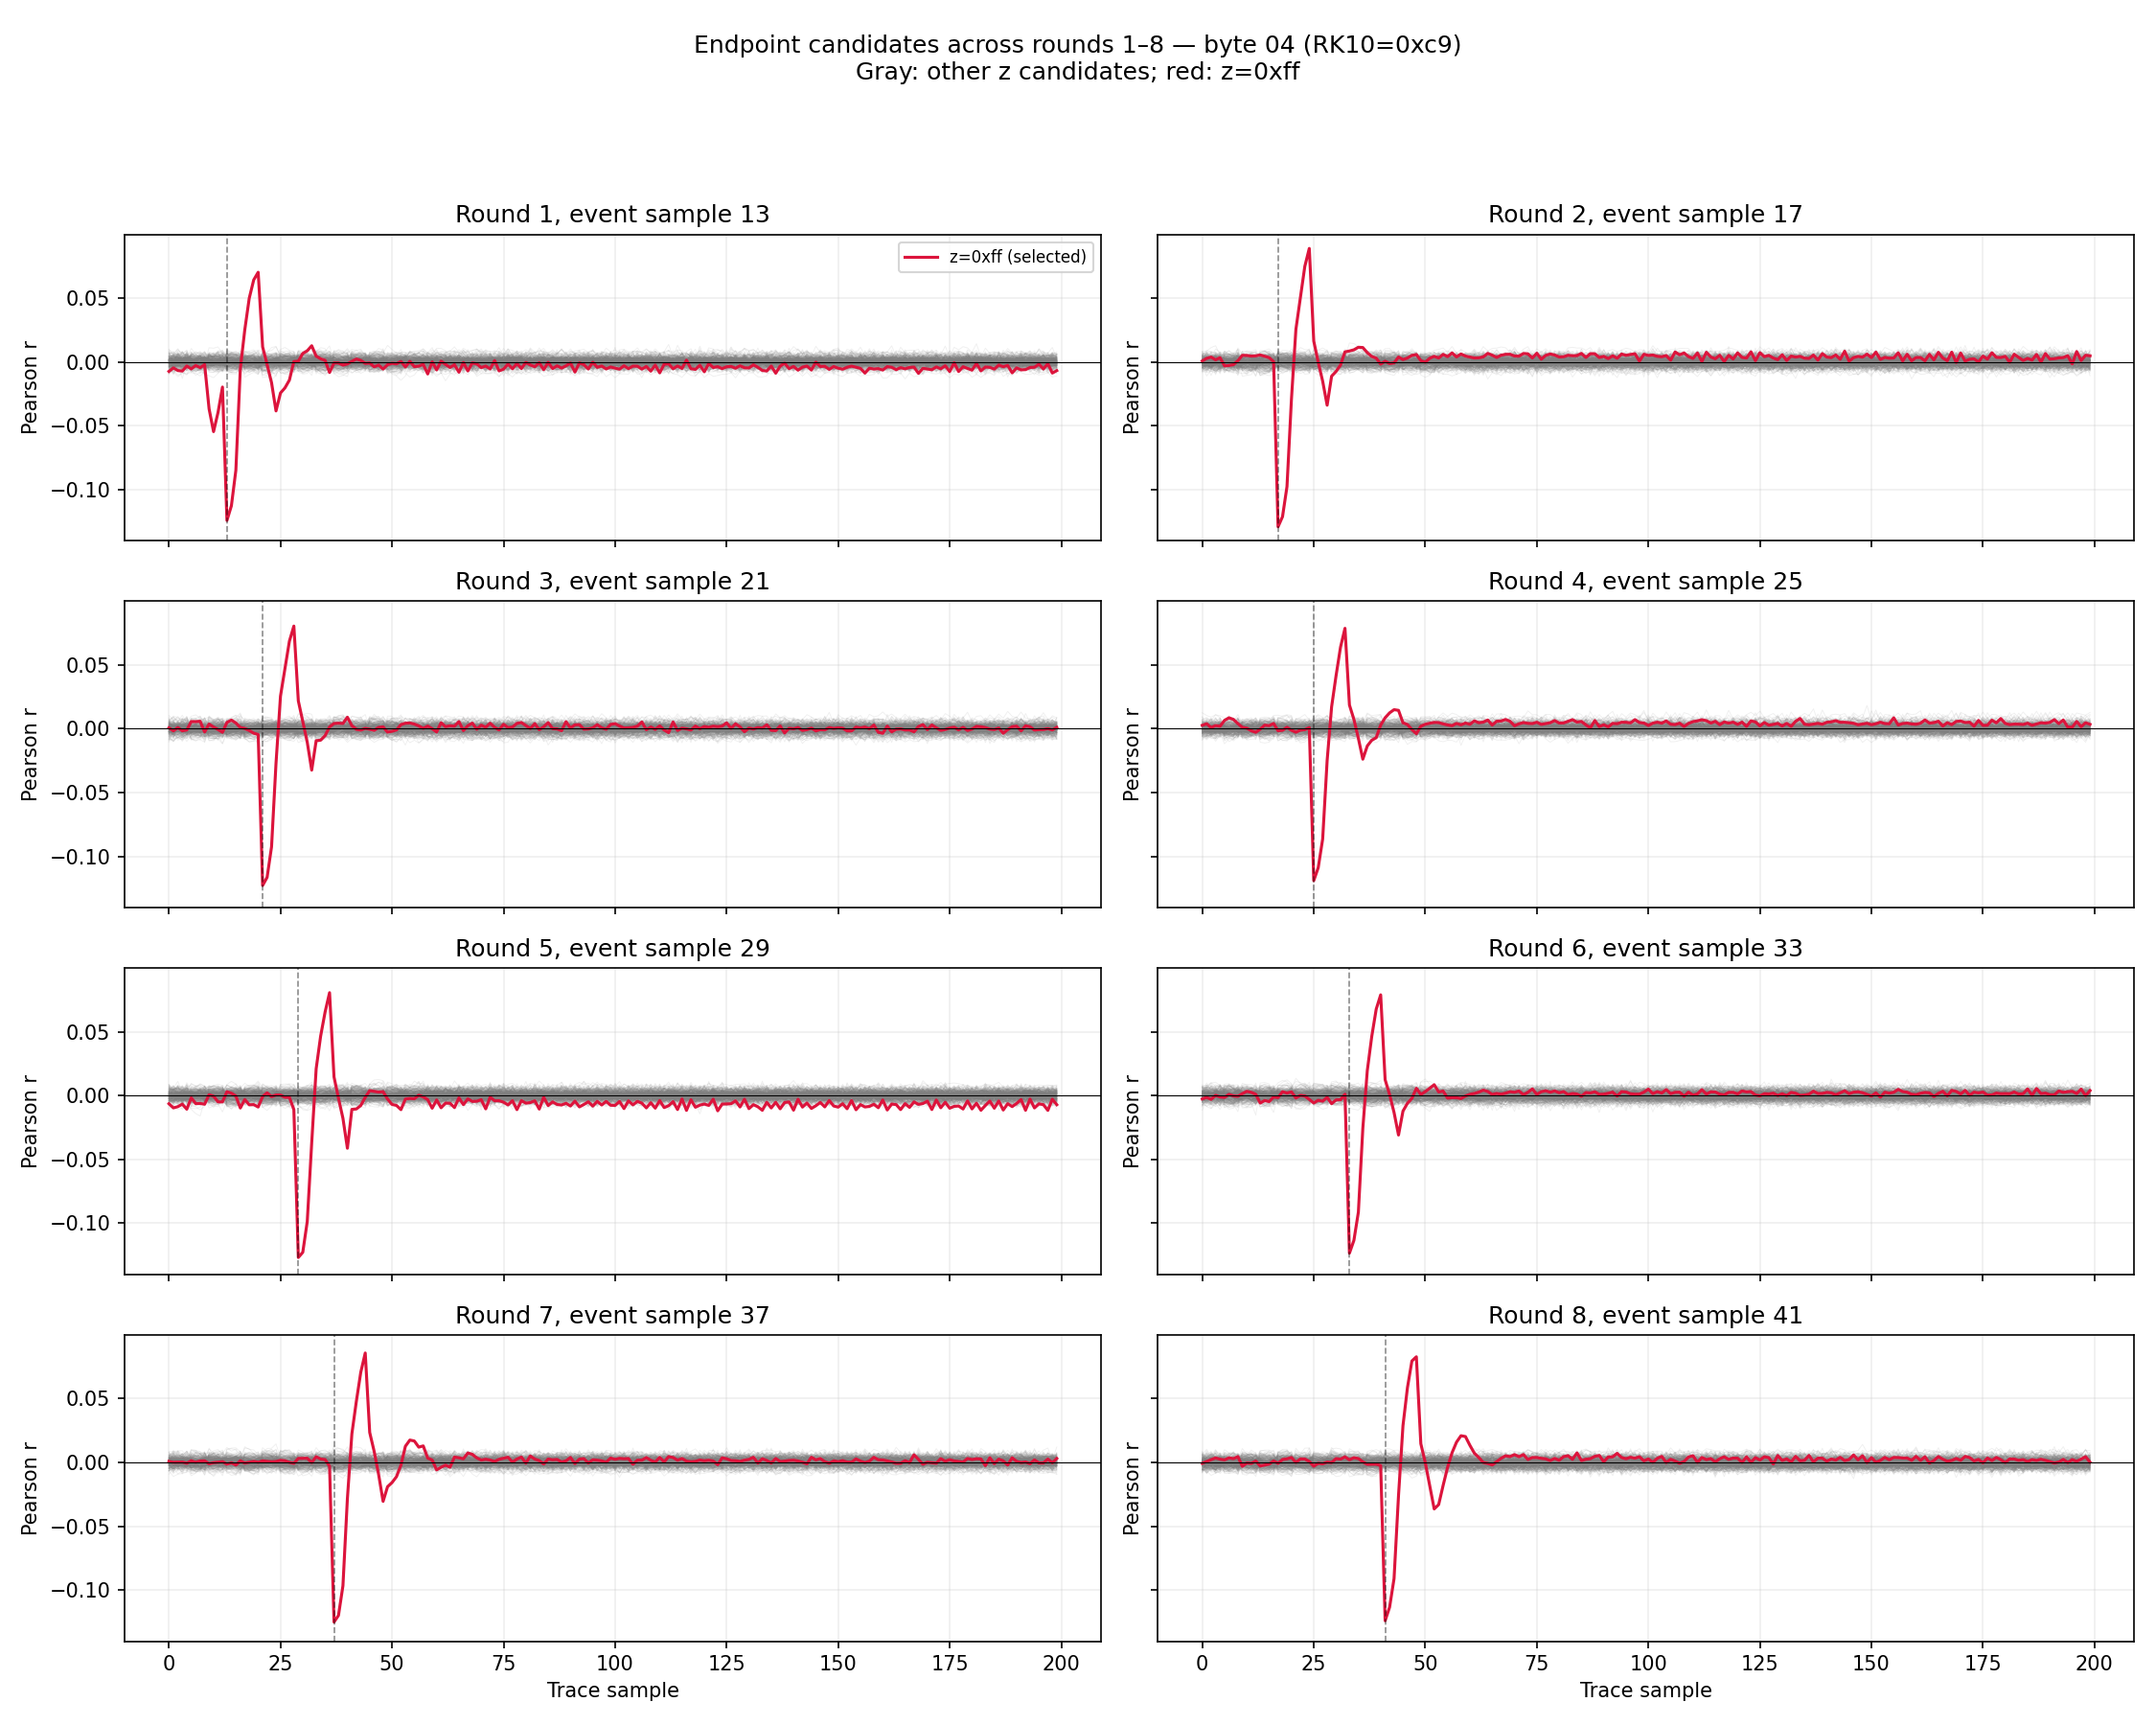
\includegraphics[width=0.96\textwidth]{actual_round10_correlation_plots/byte_04.png}
\caption{Task 3: endpoint-candidate correlations for byte 04 across rounds 1--8. Red curves mark the selected $z=\texttt{0xFF}$; dashed lines mark the detected event samples.}
\label{fig:task3-byte-04}
\end{figure}

\clearpage

\begin{figure}[H]
\centering
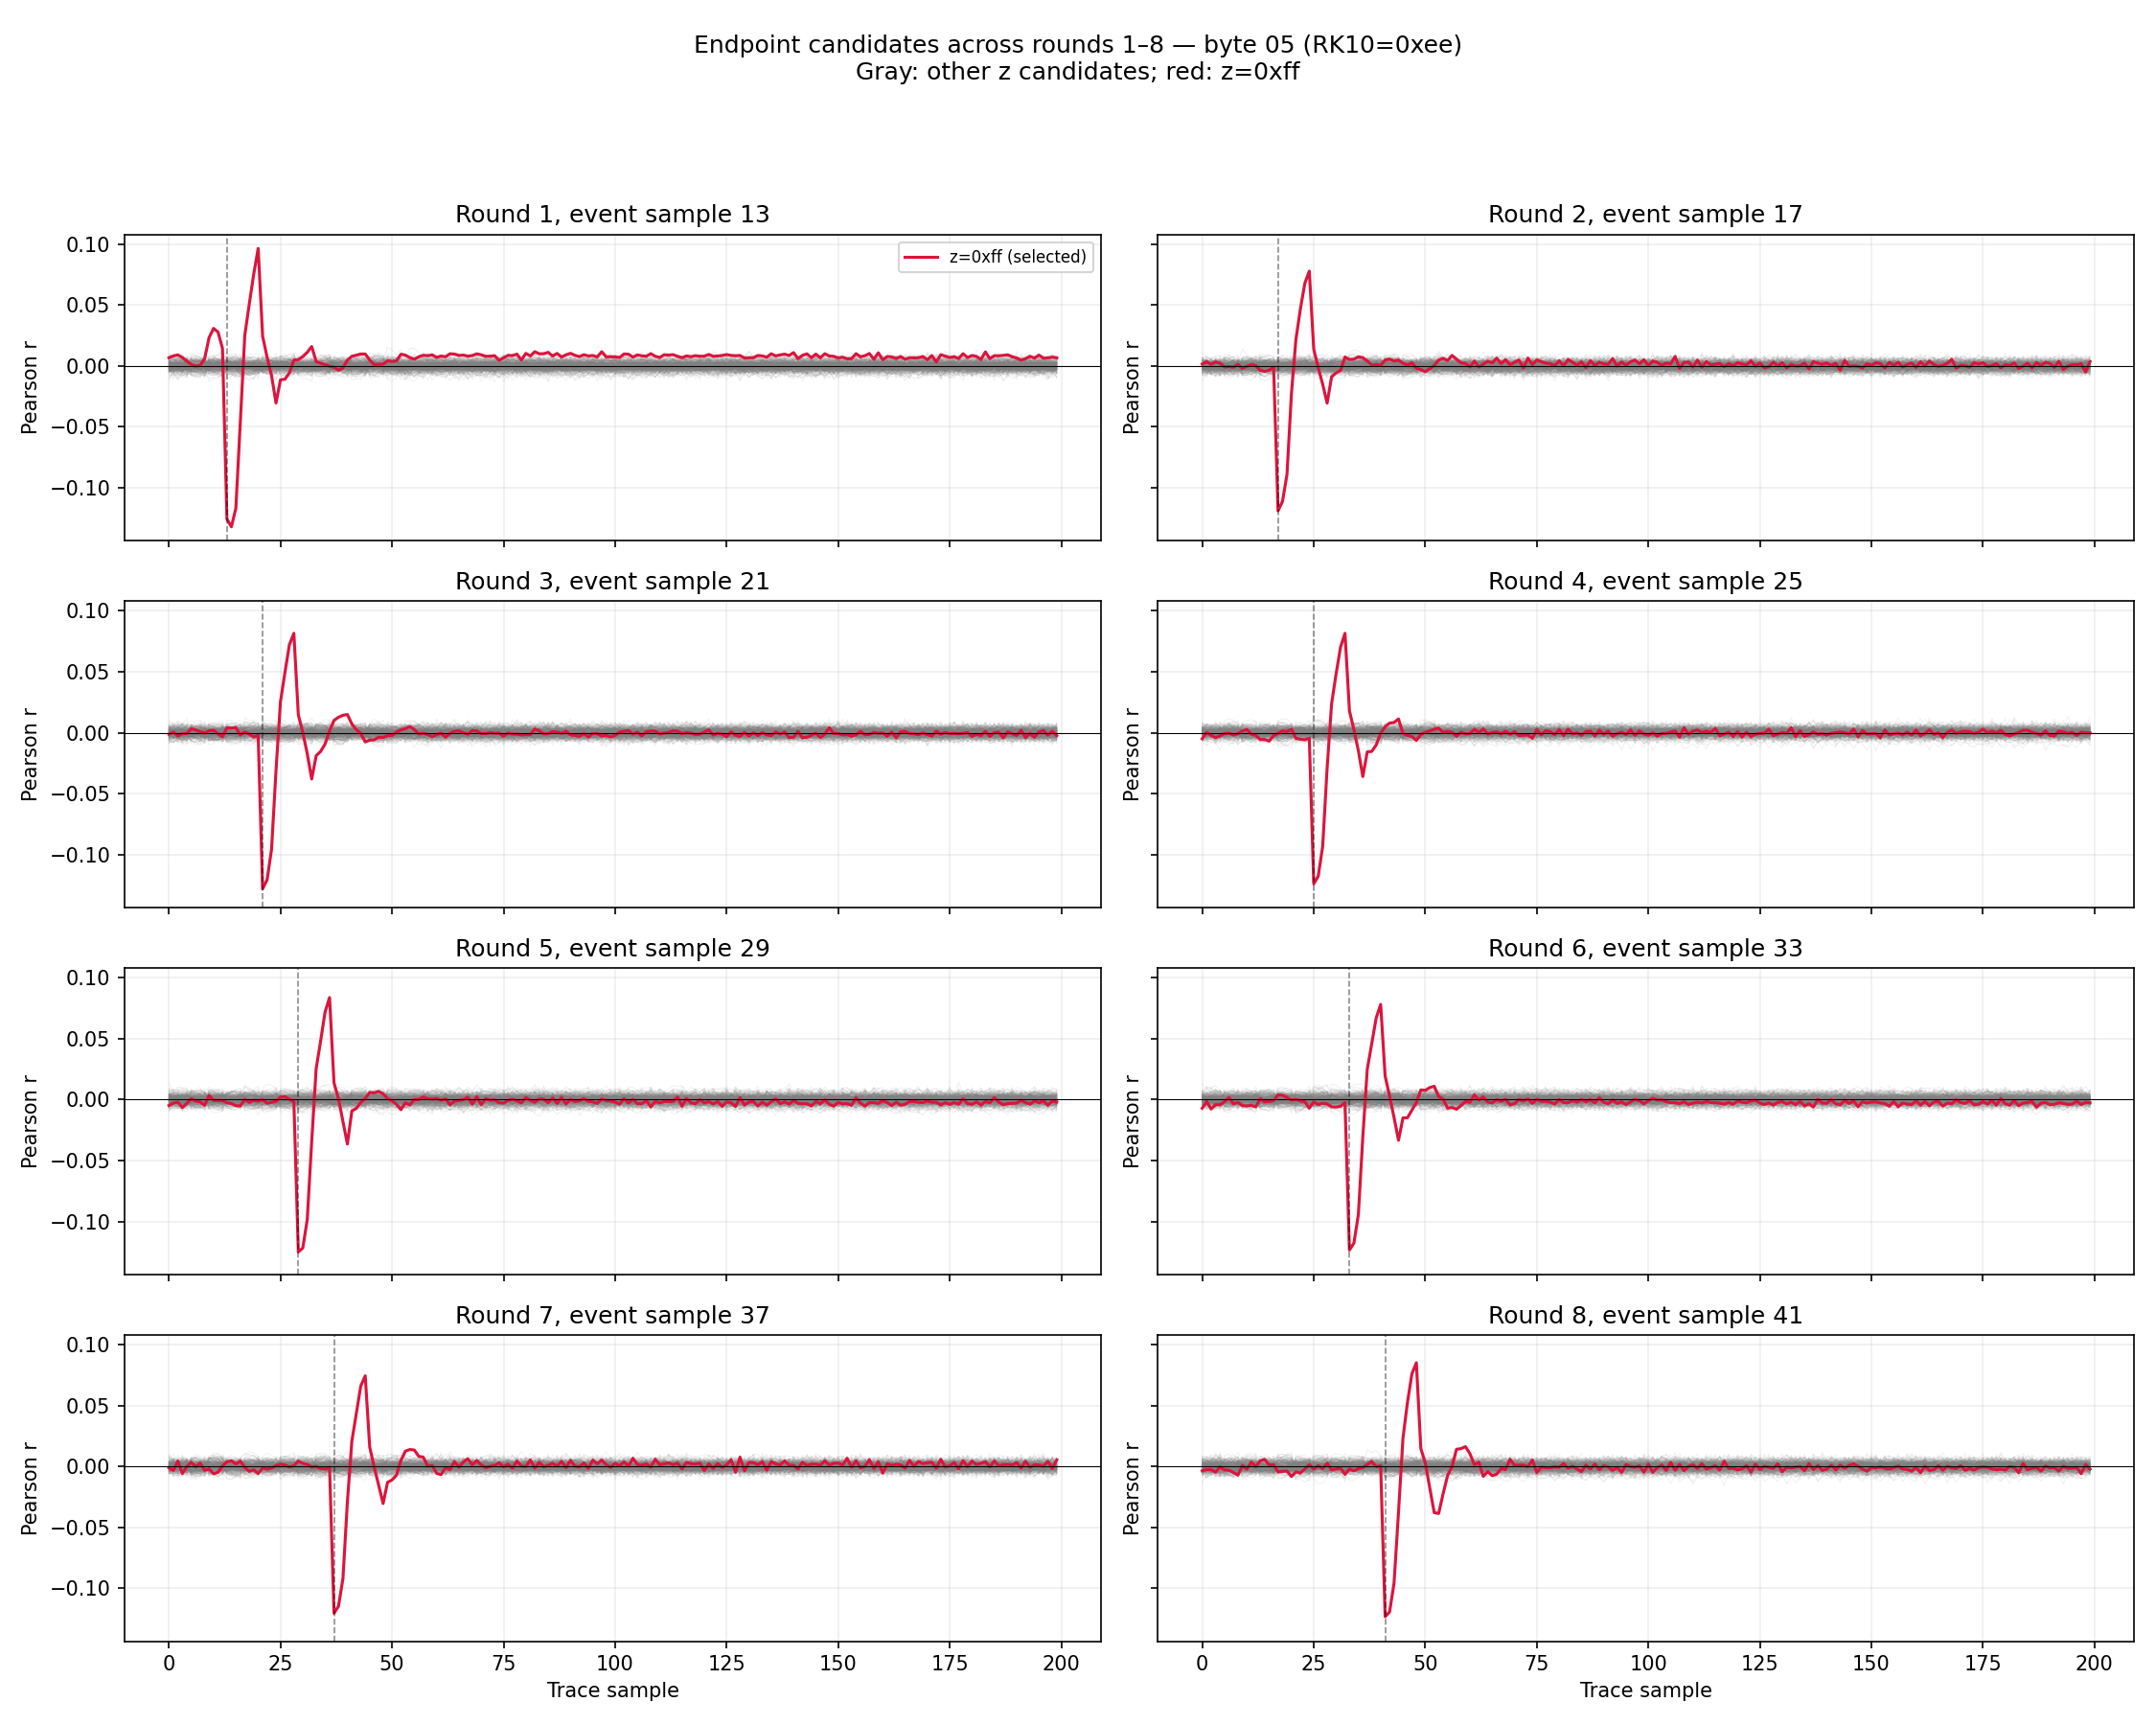
\includegraphics[width=0.96\textwidth]{actual_round10_correlation_plots/byte_05.png}
\caption{Task 3: endpoint-candidate correlations for byte 05 across rounds 1--8. Red curves mark the selected $z=\texttt{0xFF}$; dashed lines mark the detected event samples.}
\label{fig:task3-byte-05}
\end{figure}

\clearpage

\begin{figure}[H]
\centering
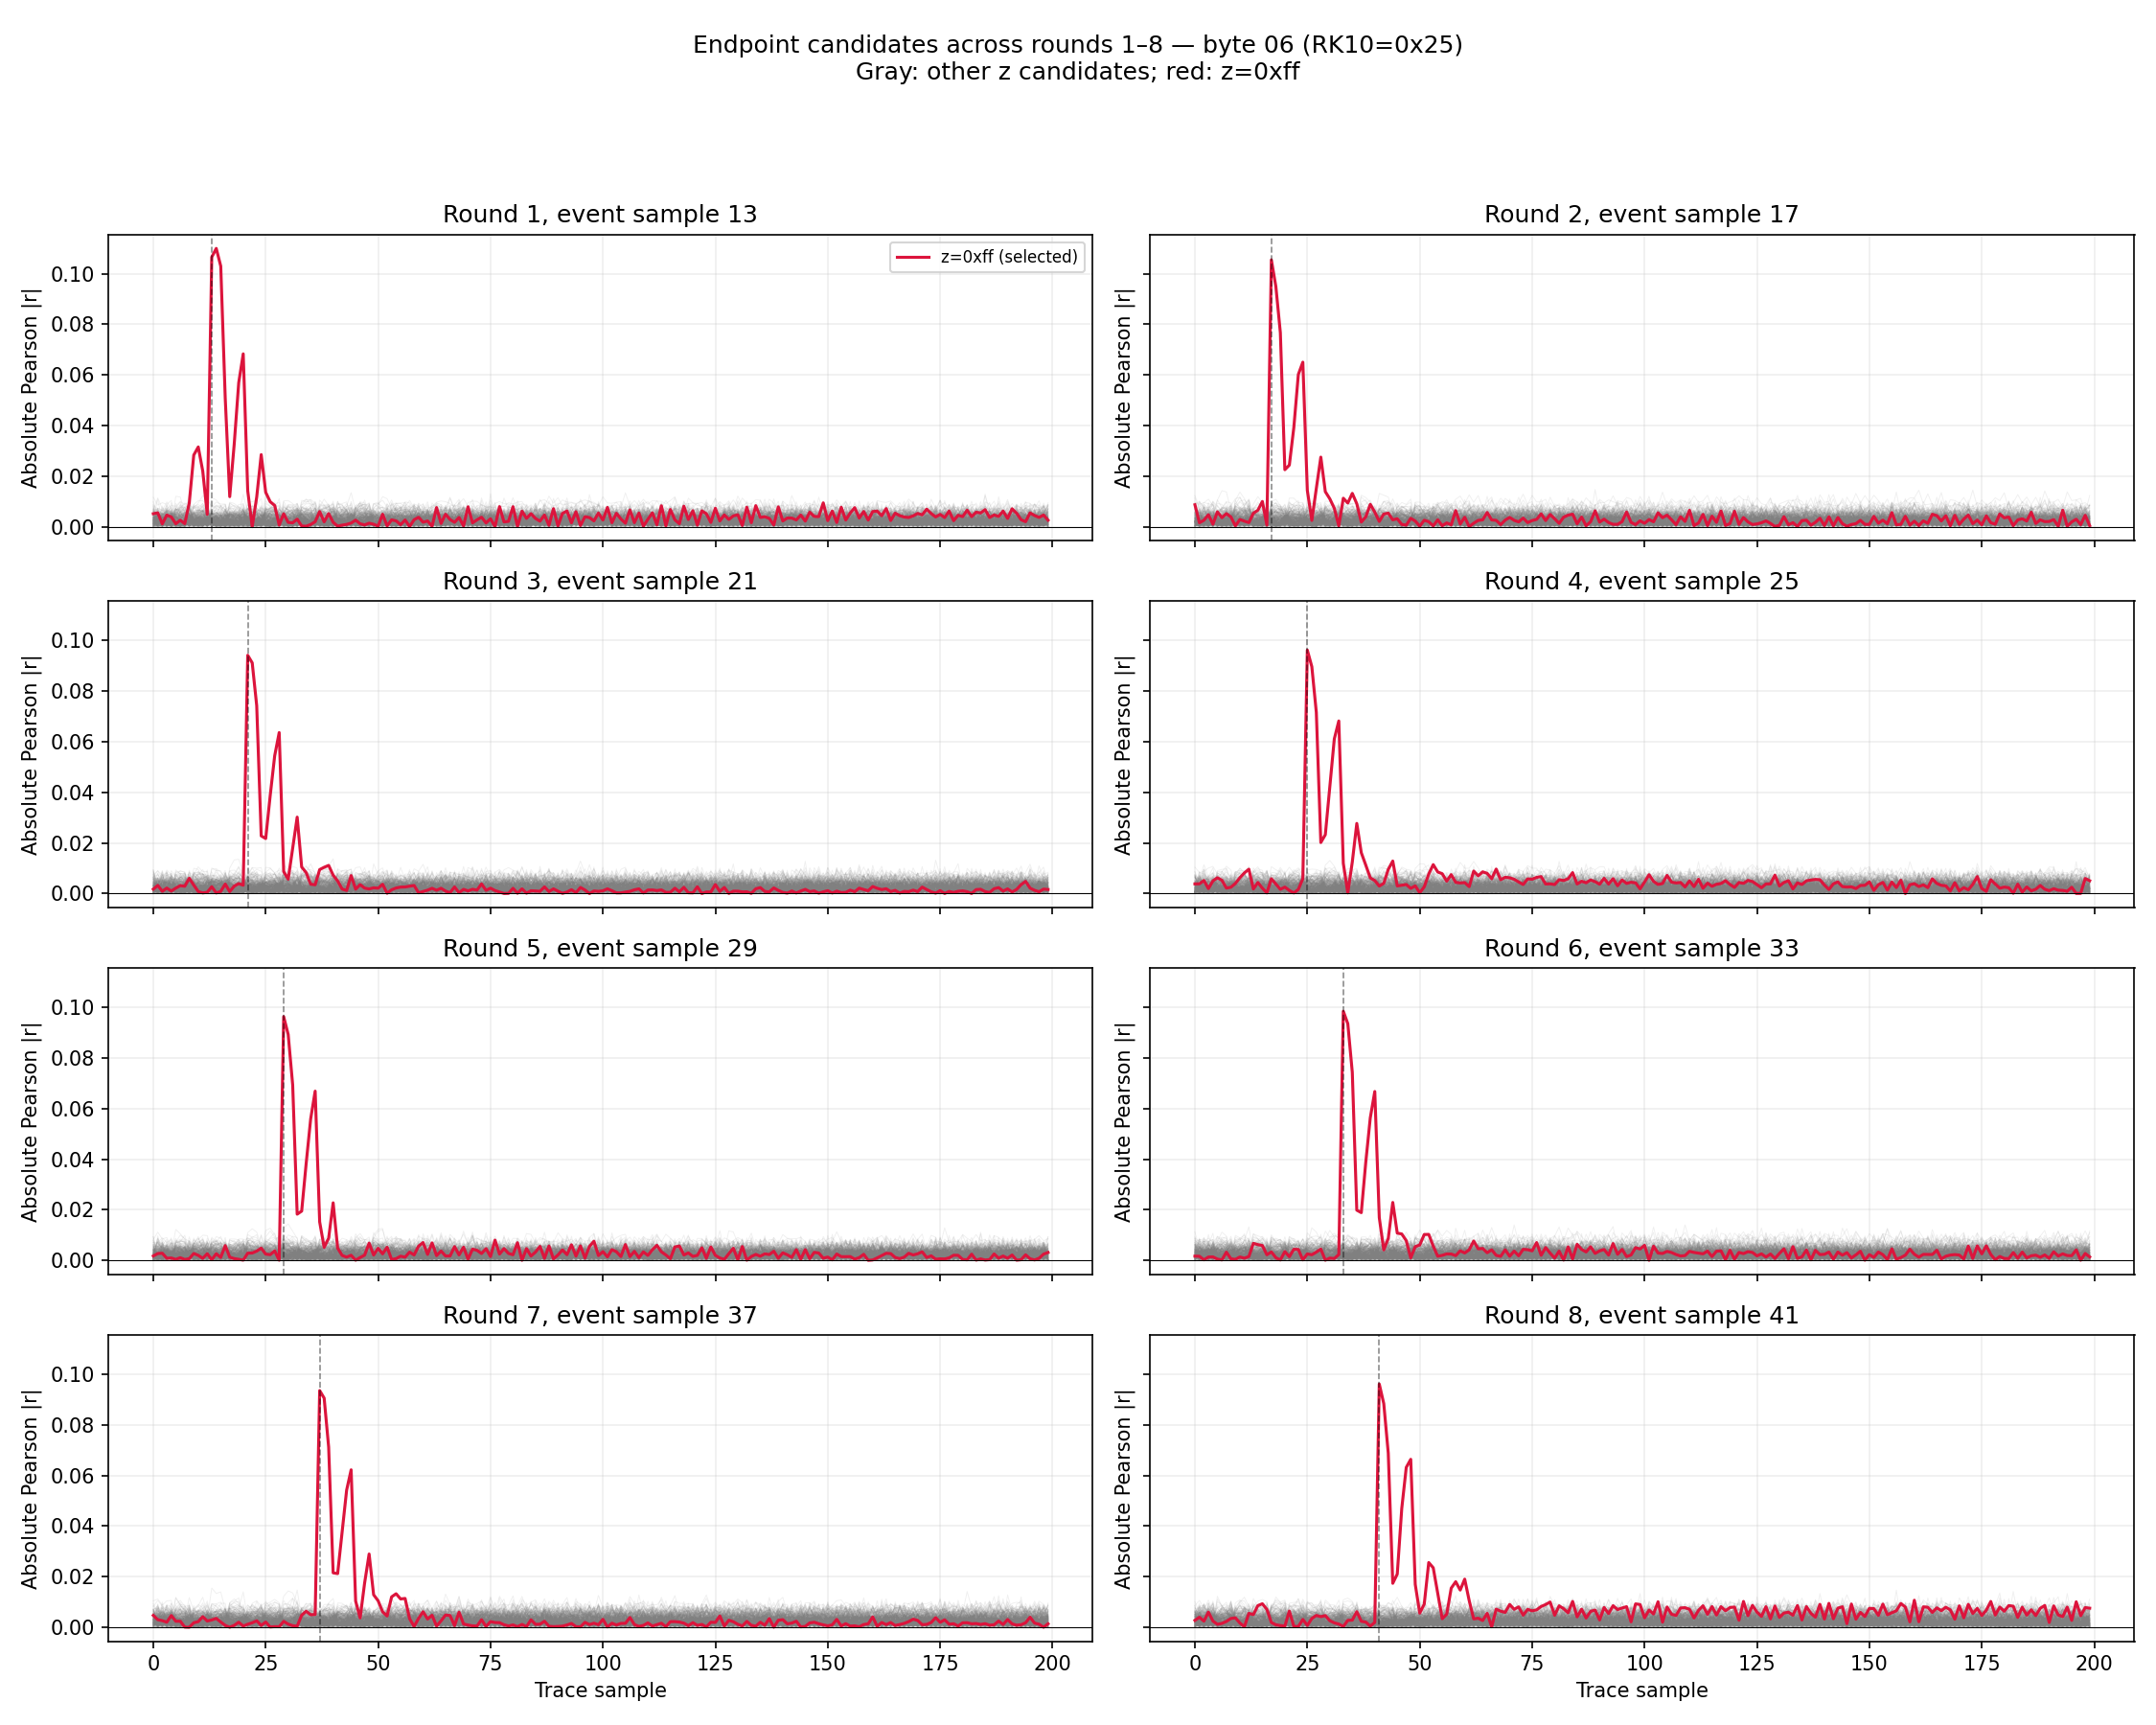
\includegraphics[width=0.96\textwidth]{actual_round10_correlation_plots/byte_06.png}
\caption{Task 3: endpoint-candidate correlations for byte 06 across rounds 1--8. Red curves mark the selected $z=\texttt{0xFF}$; dashed lines mark the detected event samples.}
\label{fig:task3-byte-06}
\end{figure}

\clearpage

\begin{figure}[H]
\centering
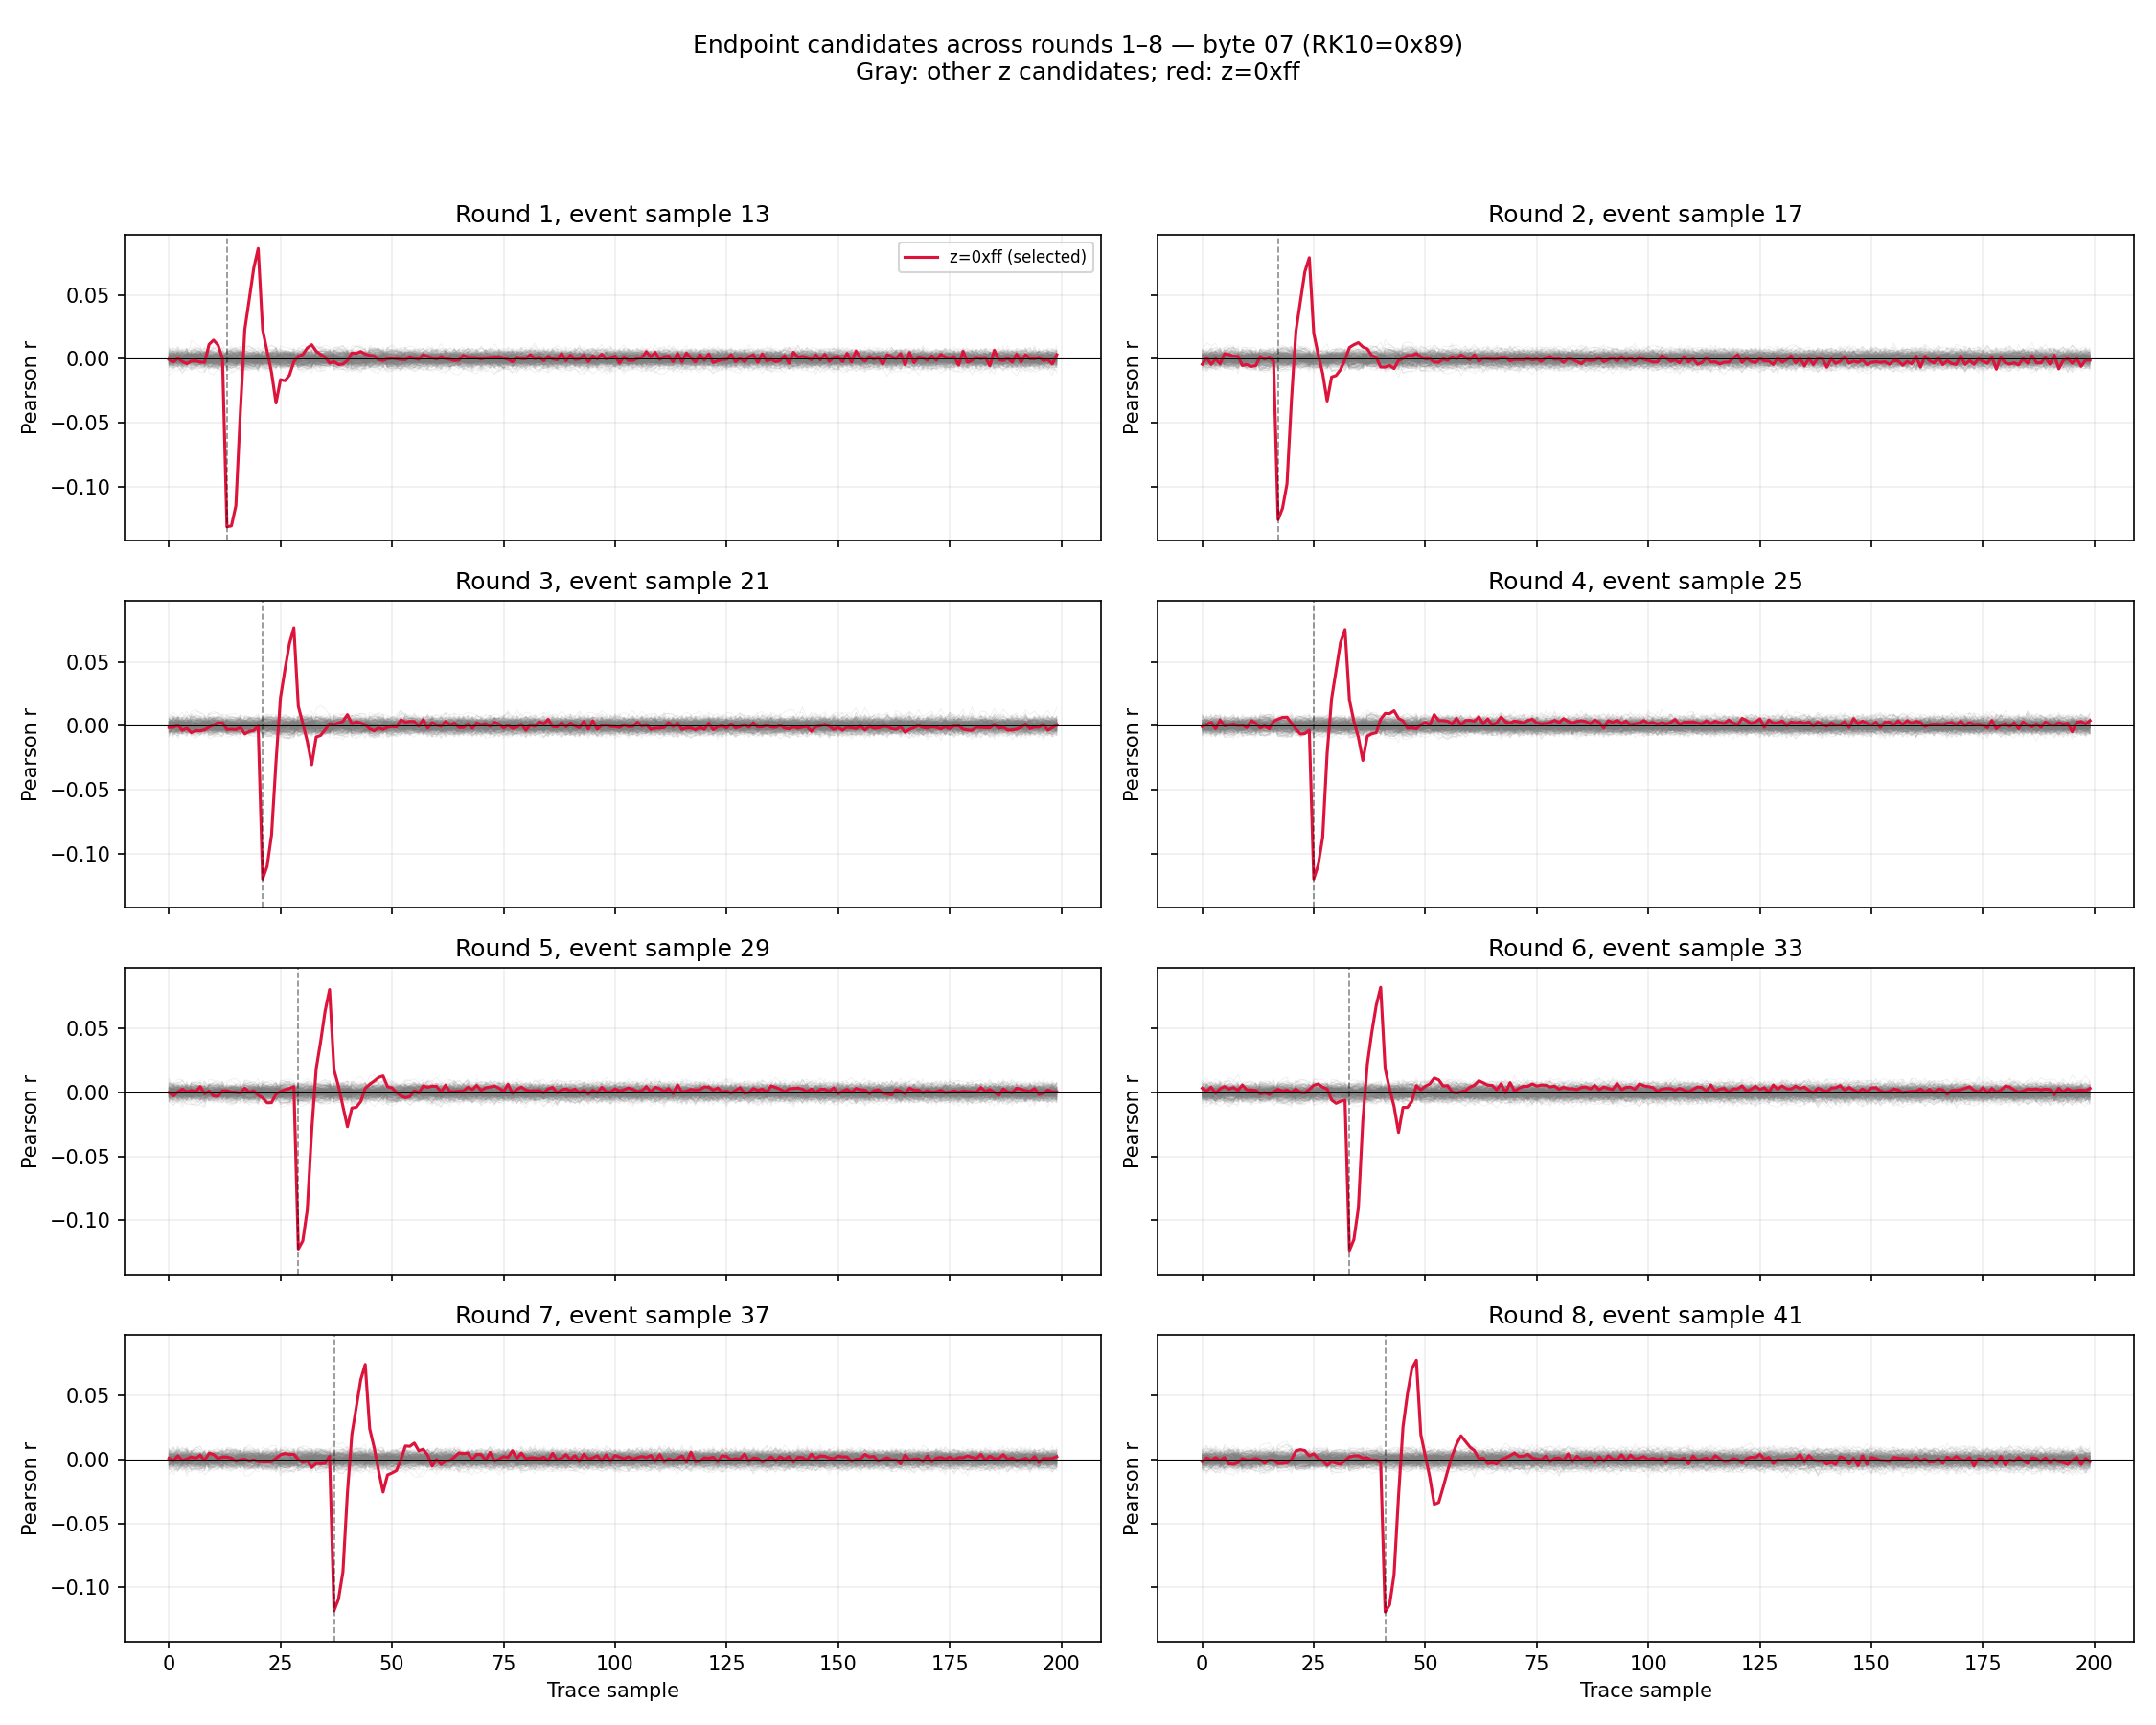
\includegraphics[width=0.96\textwidth]{actual_round10_correlation_plots/byte_07.png}
\caption{Task 3: endpoint-candidate correlations for byte 07 across rounds 1--8. Red curves mark the selected $z=\texttt{0xFF}$; dashed lines mark the detected event samples.}
\label{fig:task3-byte-07}
\end{figure}

\clearpage

\begin{figure}[H]
\centering
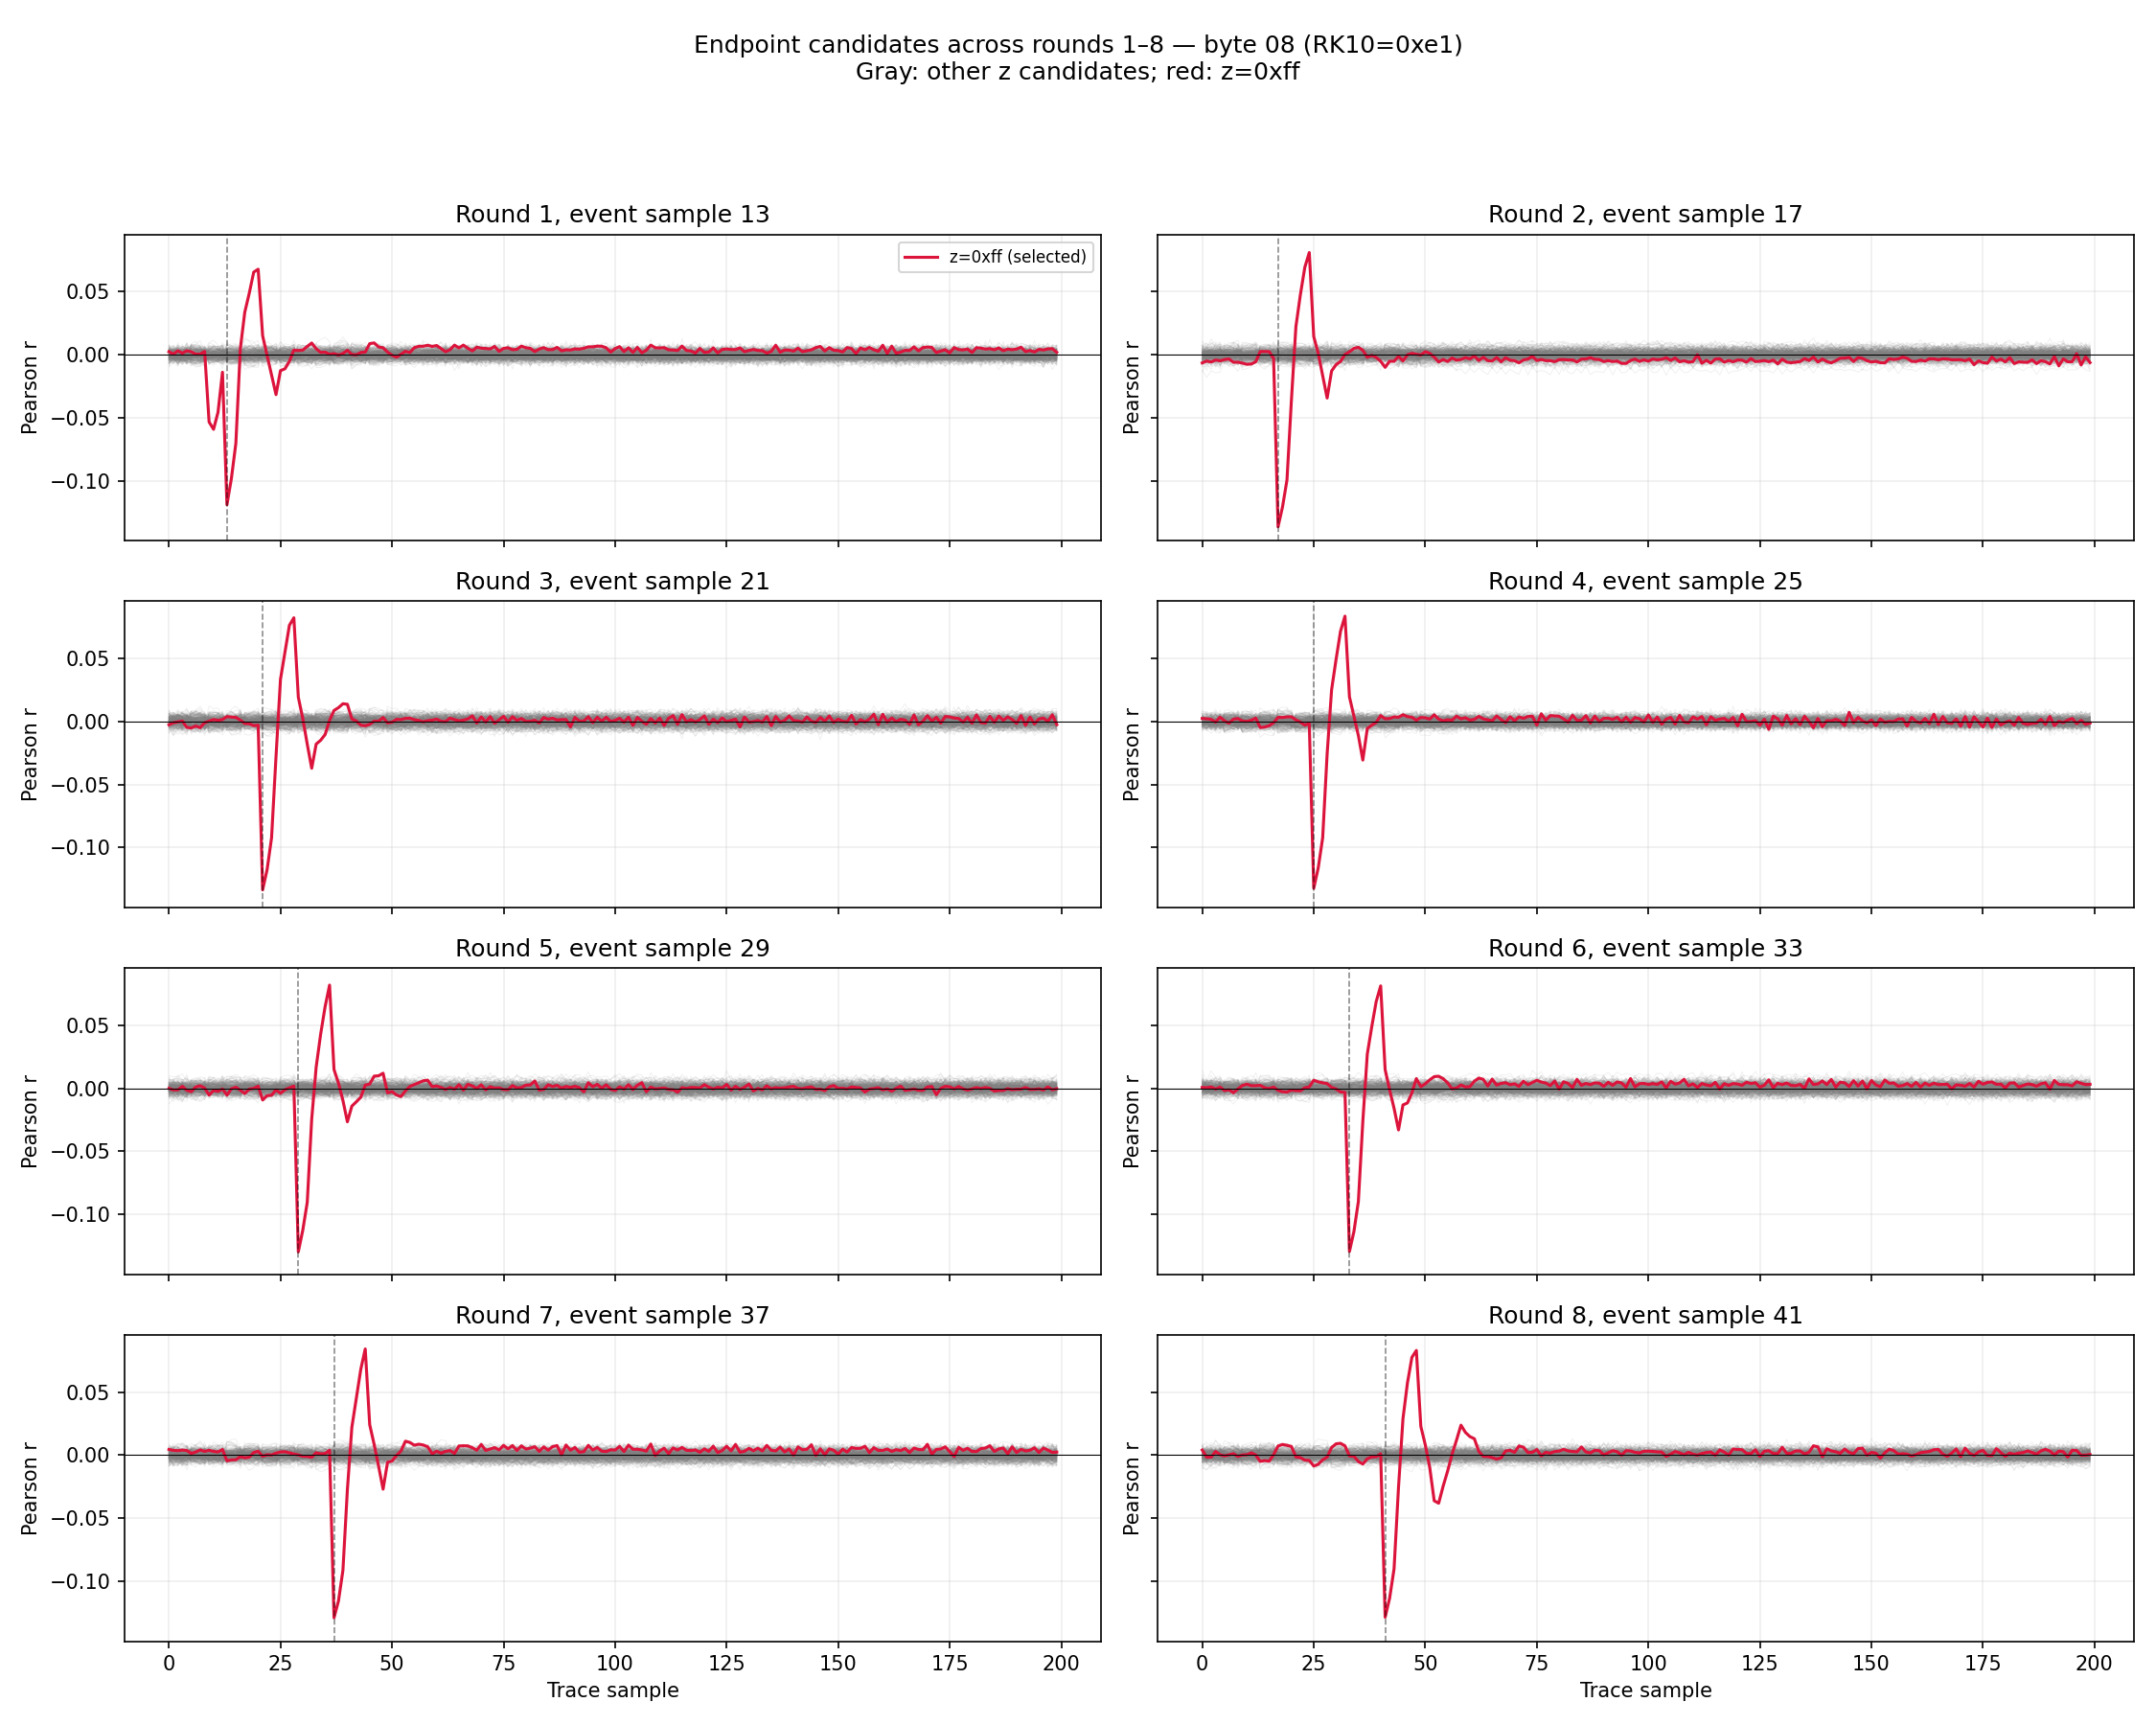
\includegraphics[width=0.96\textwidth]{actual_round10_correlation_plots/byte_08.png}
\caption{Task 3: endpoint-candidate correlations for byte 08 across rounds 1--8. Red curves mark the selected $z=\texttt{0xFF}$; dashed lines mark the detected event samples.}
\label{fig:task3-byte-08}
\end{figure}

\clearpage

\begin{figure}[H]
\centering
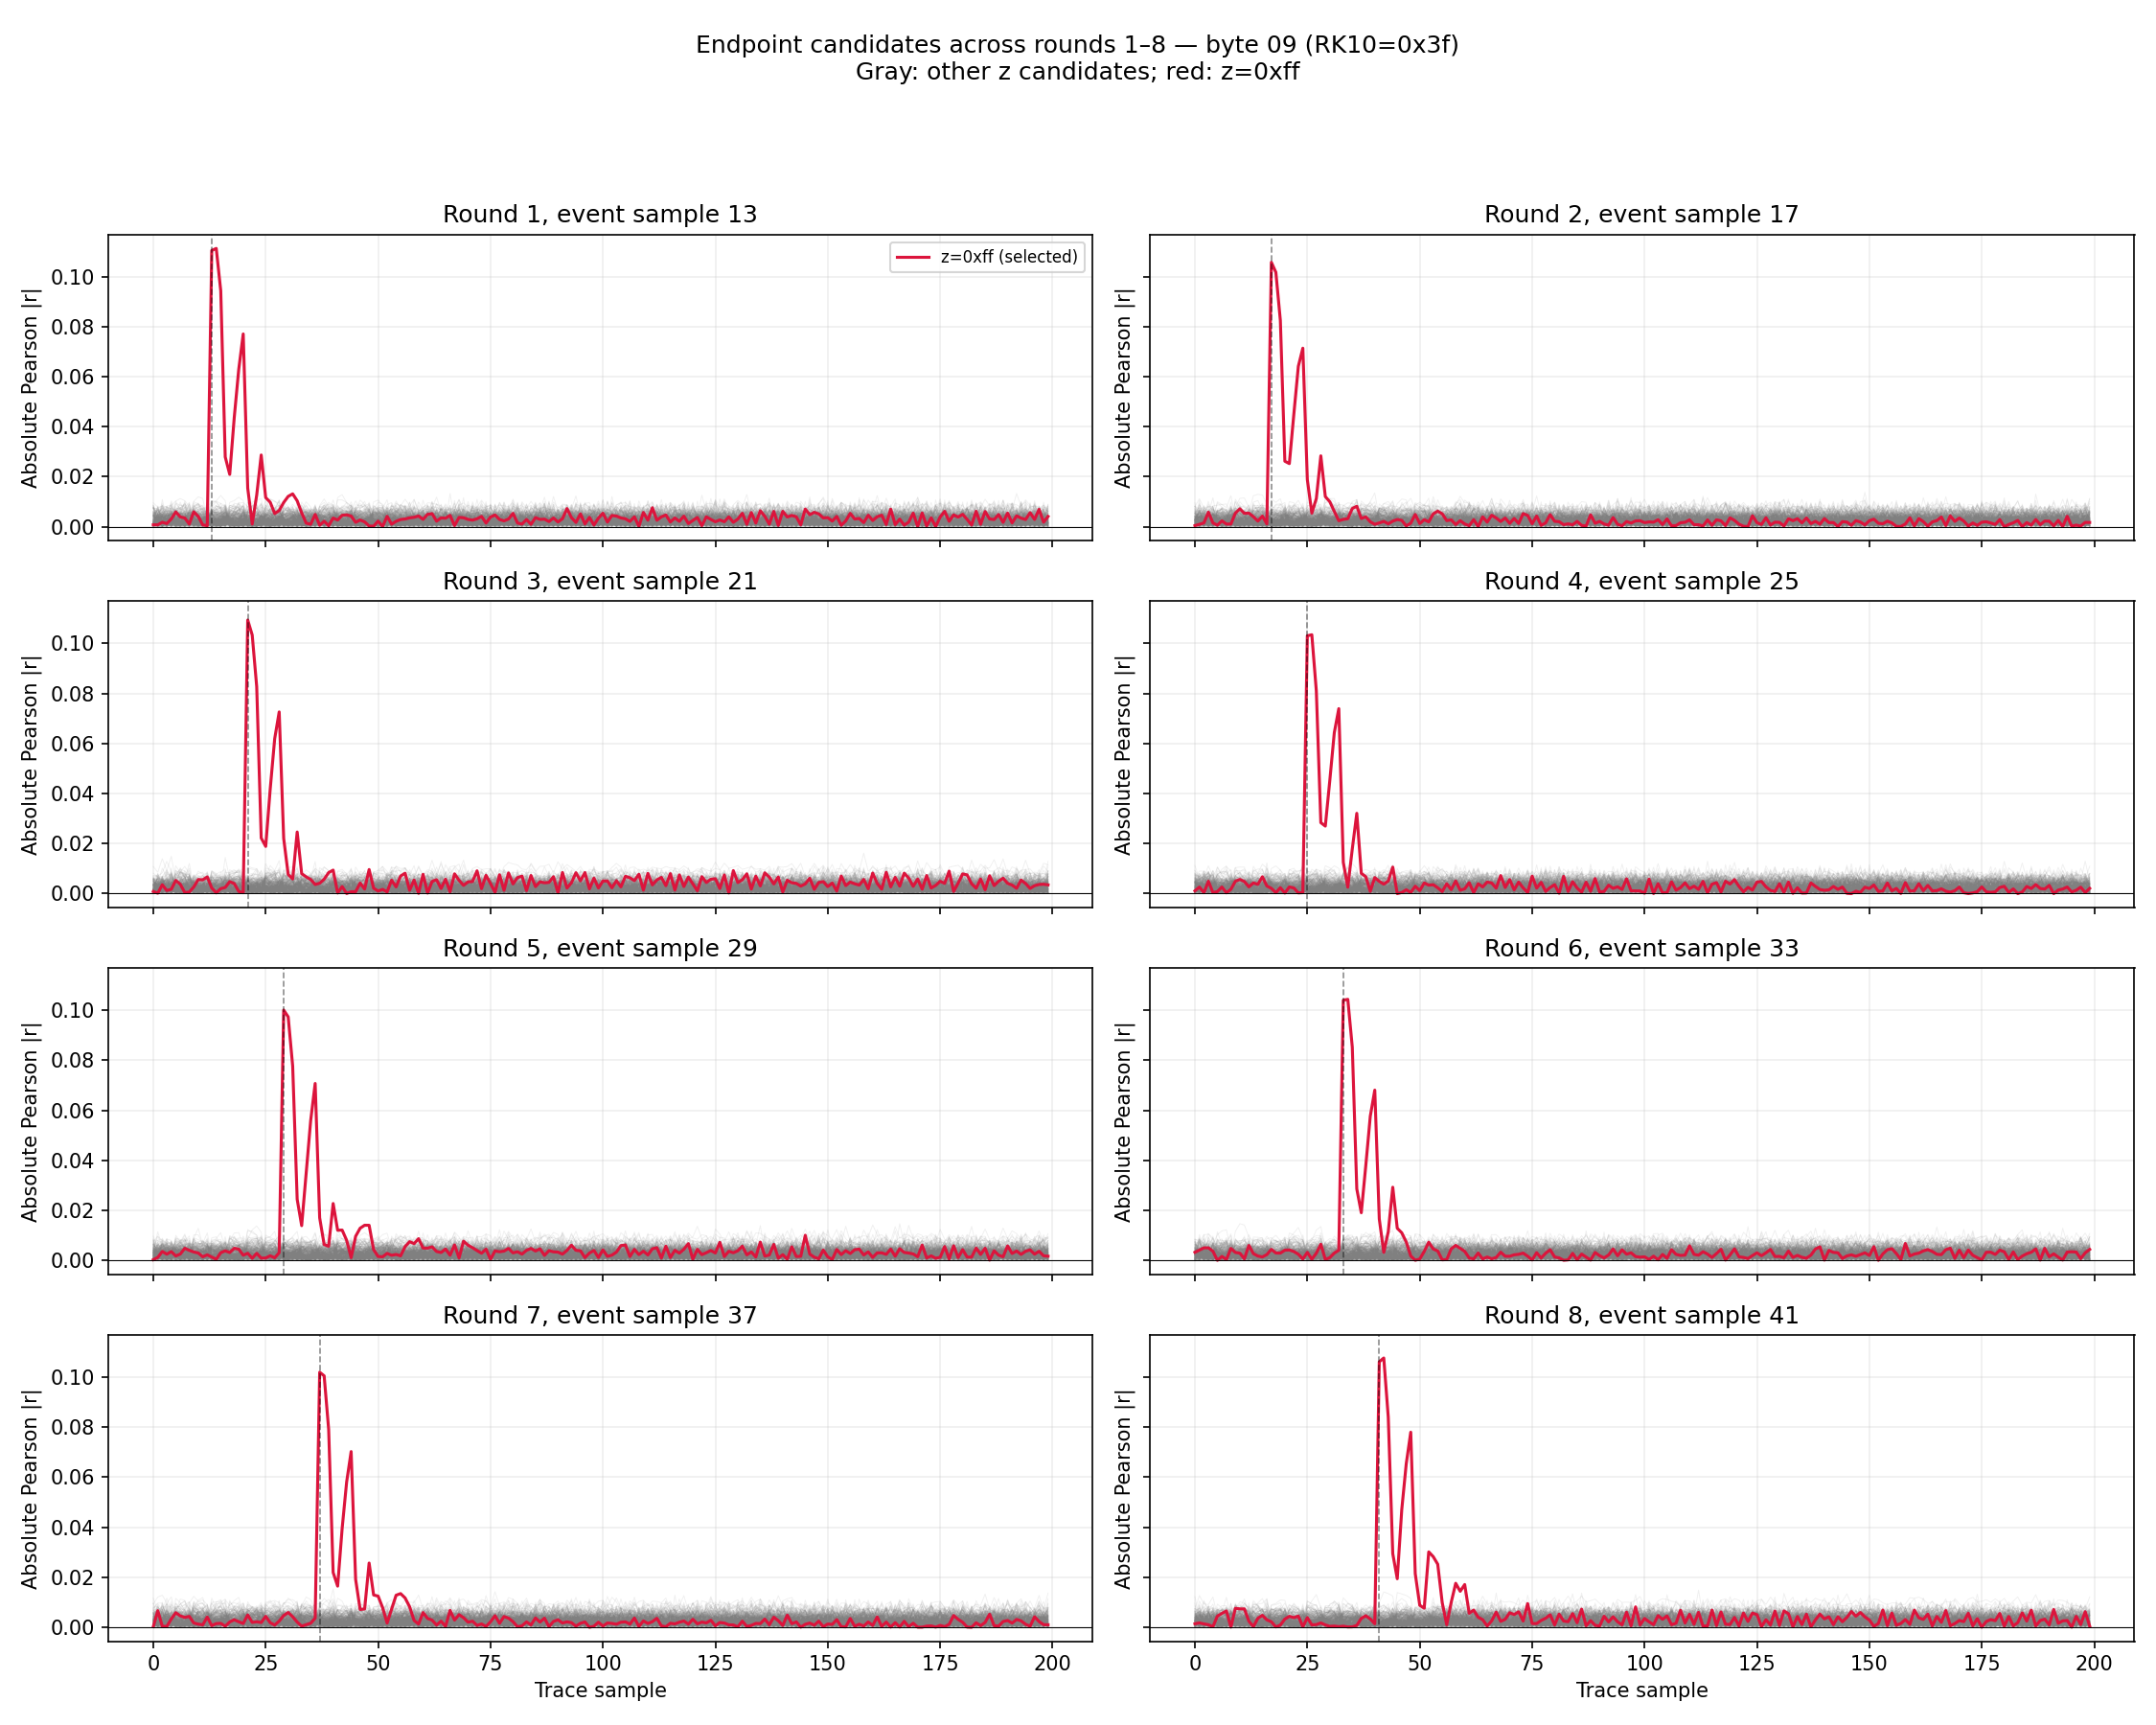
\includegraphics[width=0.96\textwidth]{actual_round10_correlation_plots/byte_09.png}
\caption{Task 3: endpoint-candidate correlations for byte 09 across rounds 1--8. Red curves mark the selected $z=\texttt{0xFF}$; dashed lines mark the detected event samples.}
\label{fig:task3-byte-09}
\end{figure}

\clearpage

\begin{figure}[H]
\centering
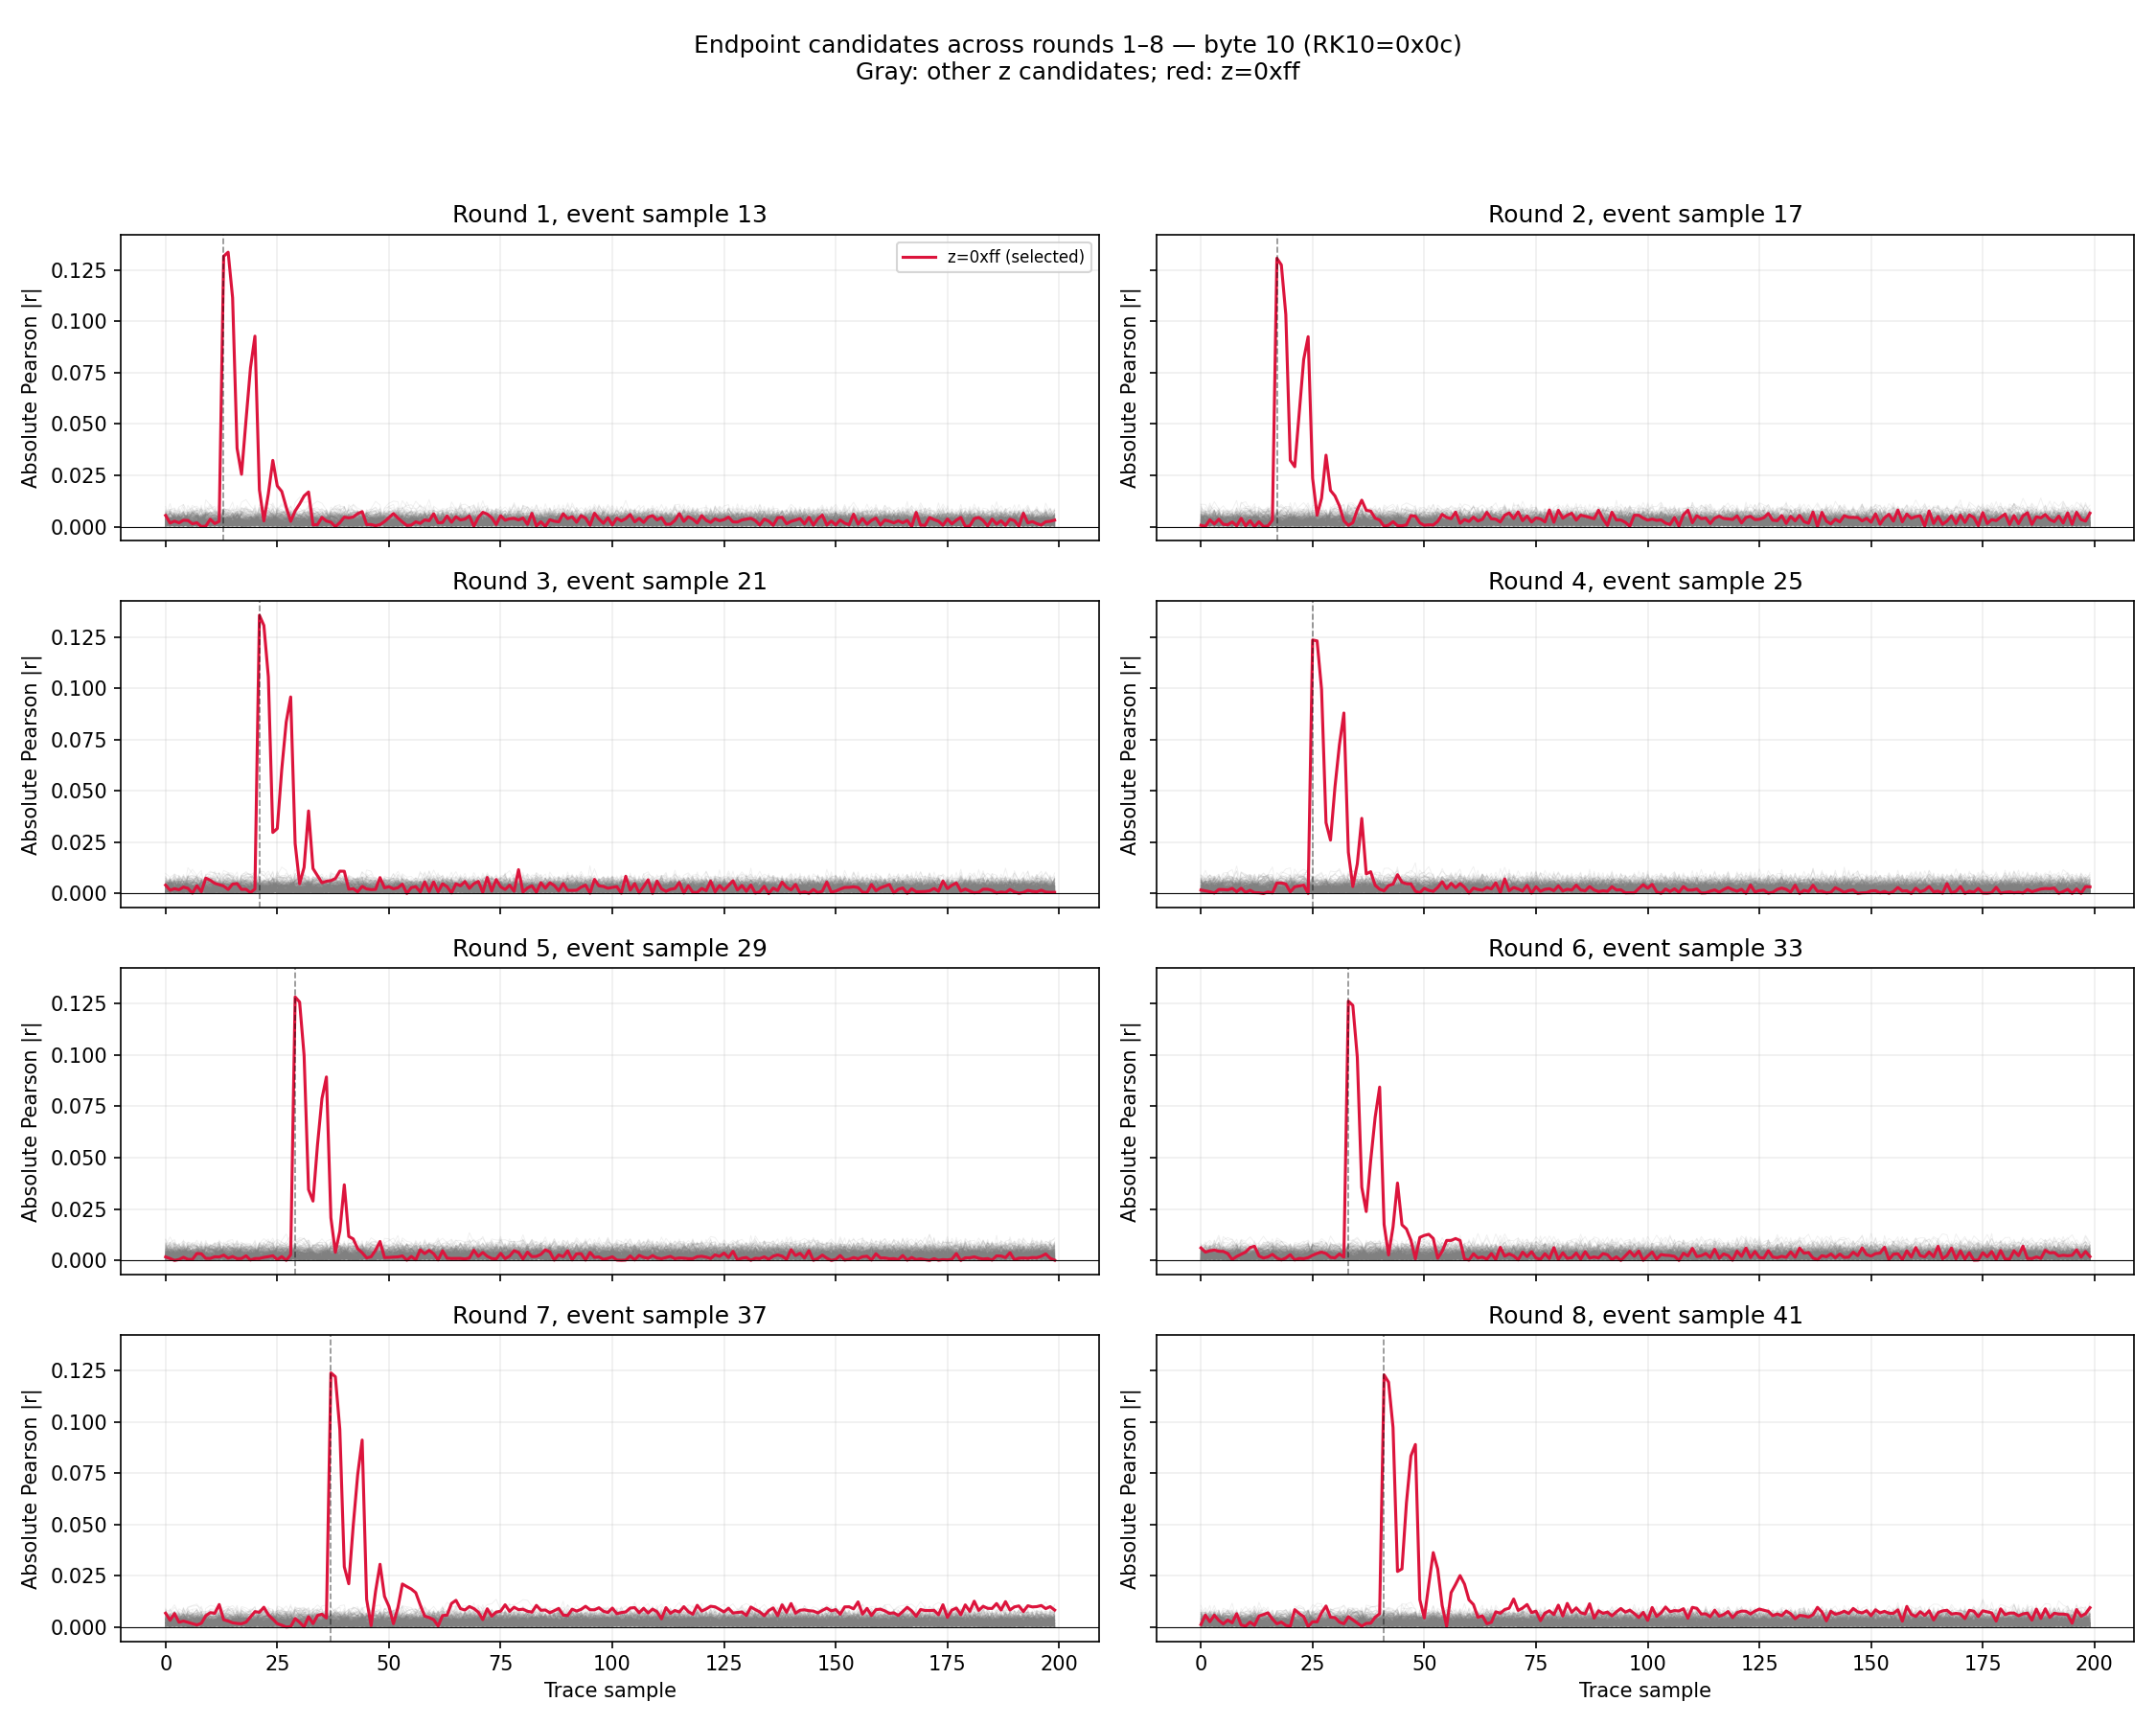
\includegraphics[width=0.96\textwidth]{actual_round10_correlation_plots/byte_10.png}
\caption{Task 3: endpoint-candidate correlations for byte 10 across rounds 1--8. Red curves mark the selected $z=\texttt{0xFF}$; dashed lines mark the detected event samples.}
\label{fig:task3-byte-10}
\end{figure}

\clearpage

\begin{figure}[H]
\centering
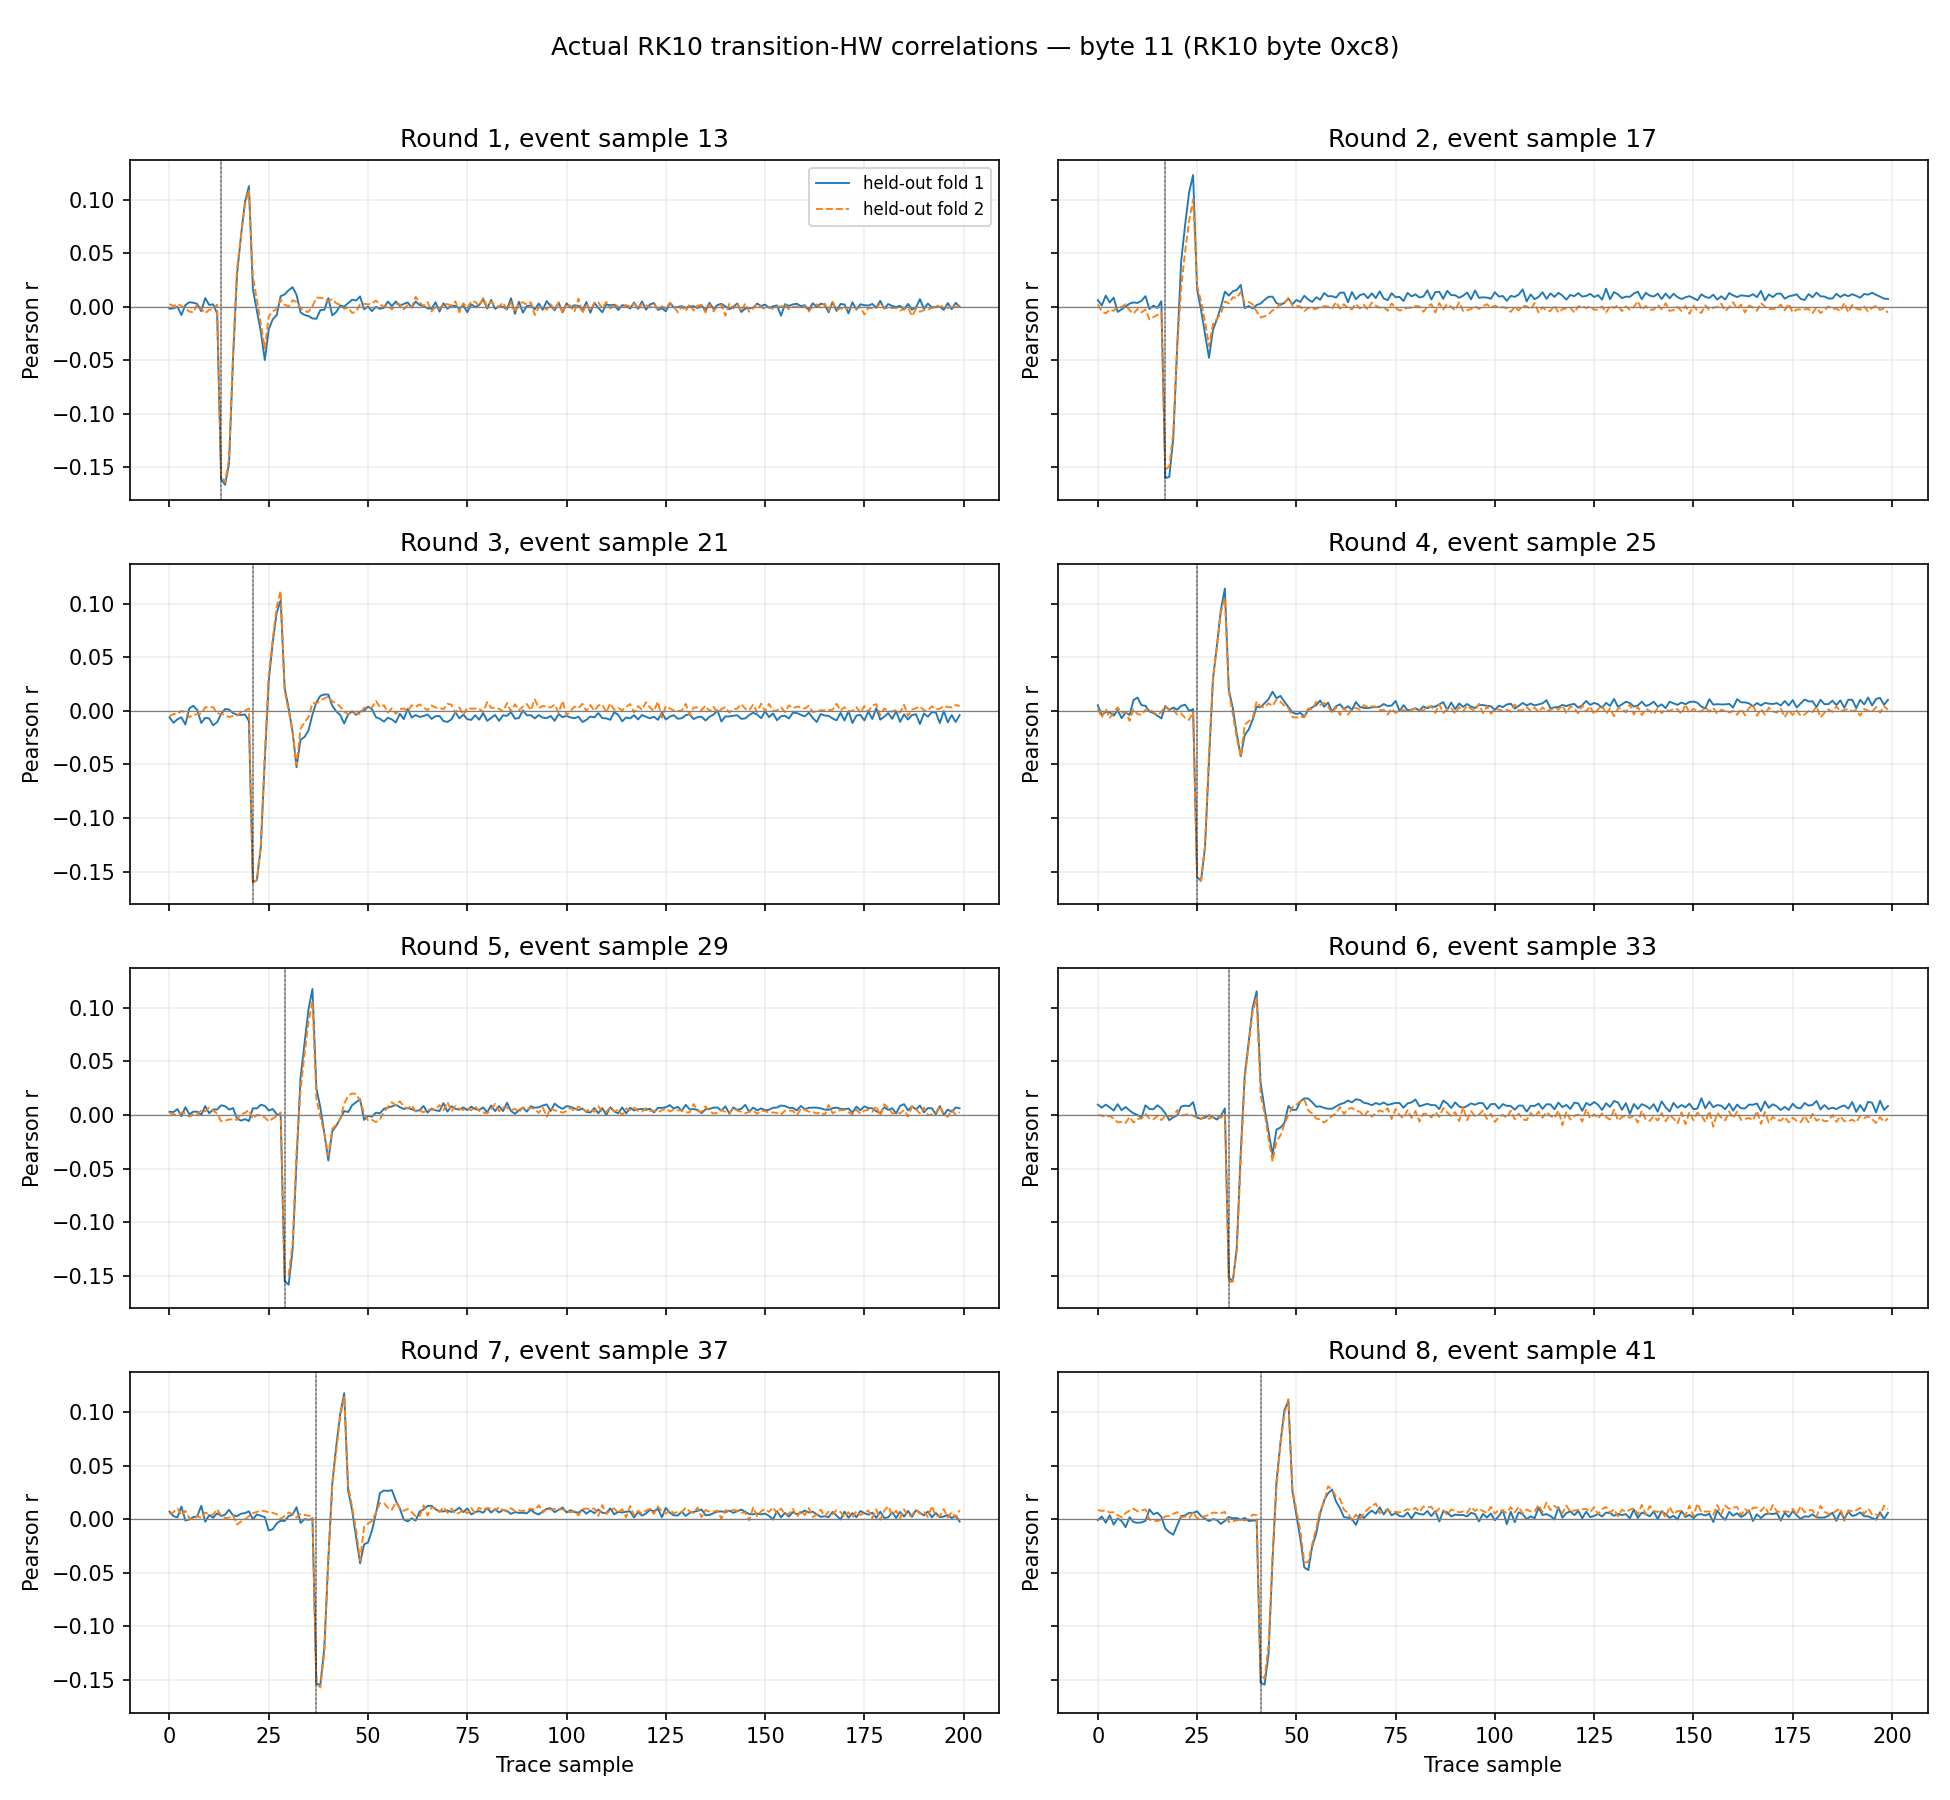
\includegraphics[width=0.96\textwidth]{actual_round10_correlation_plots/byte_11.png}
\caption{Task 3: endpoint-candidate correlations for byte 11 across rounds 1--8. Red curves mark the selected $z=\texttt{0xFF}$; dashed lines mark the detected event samples.}
\label{fig:task3-byte-11}
\end{figure}

\clearpage

\begin{figure}[H]
\centering
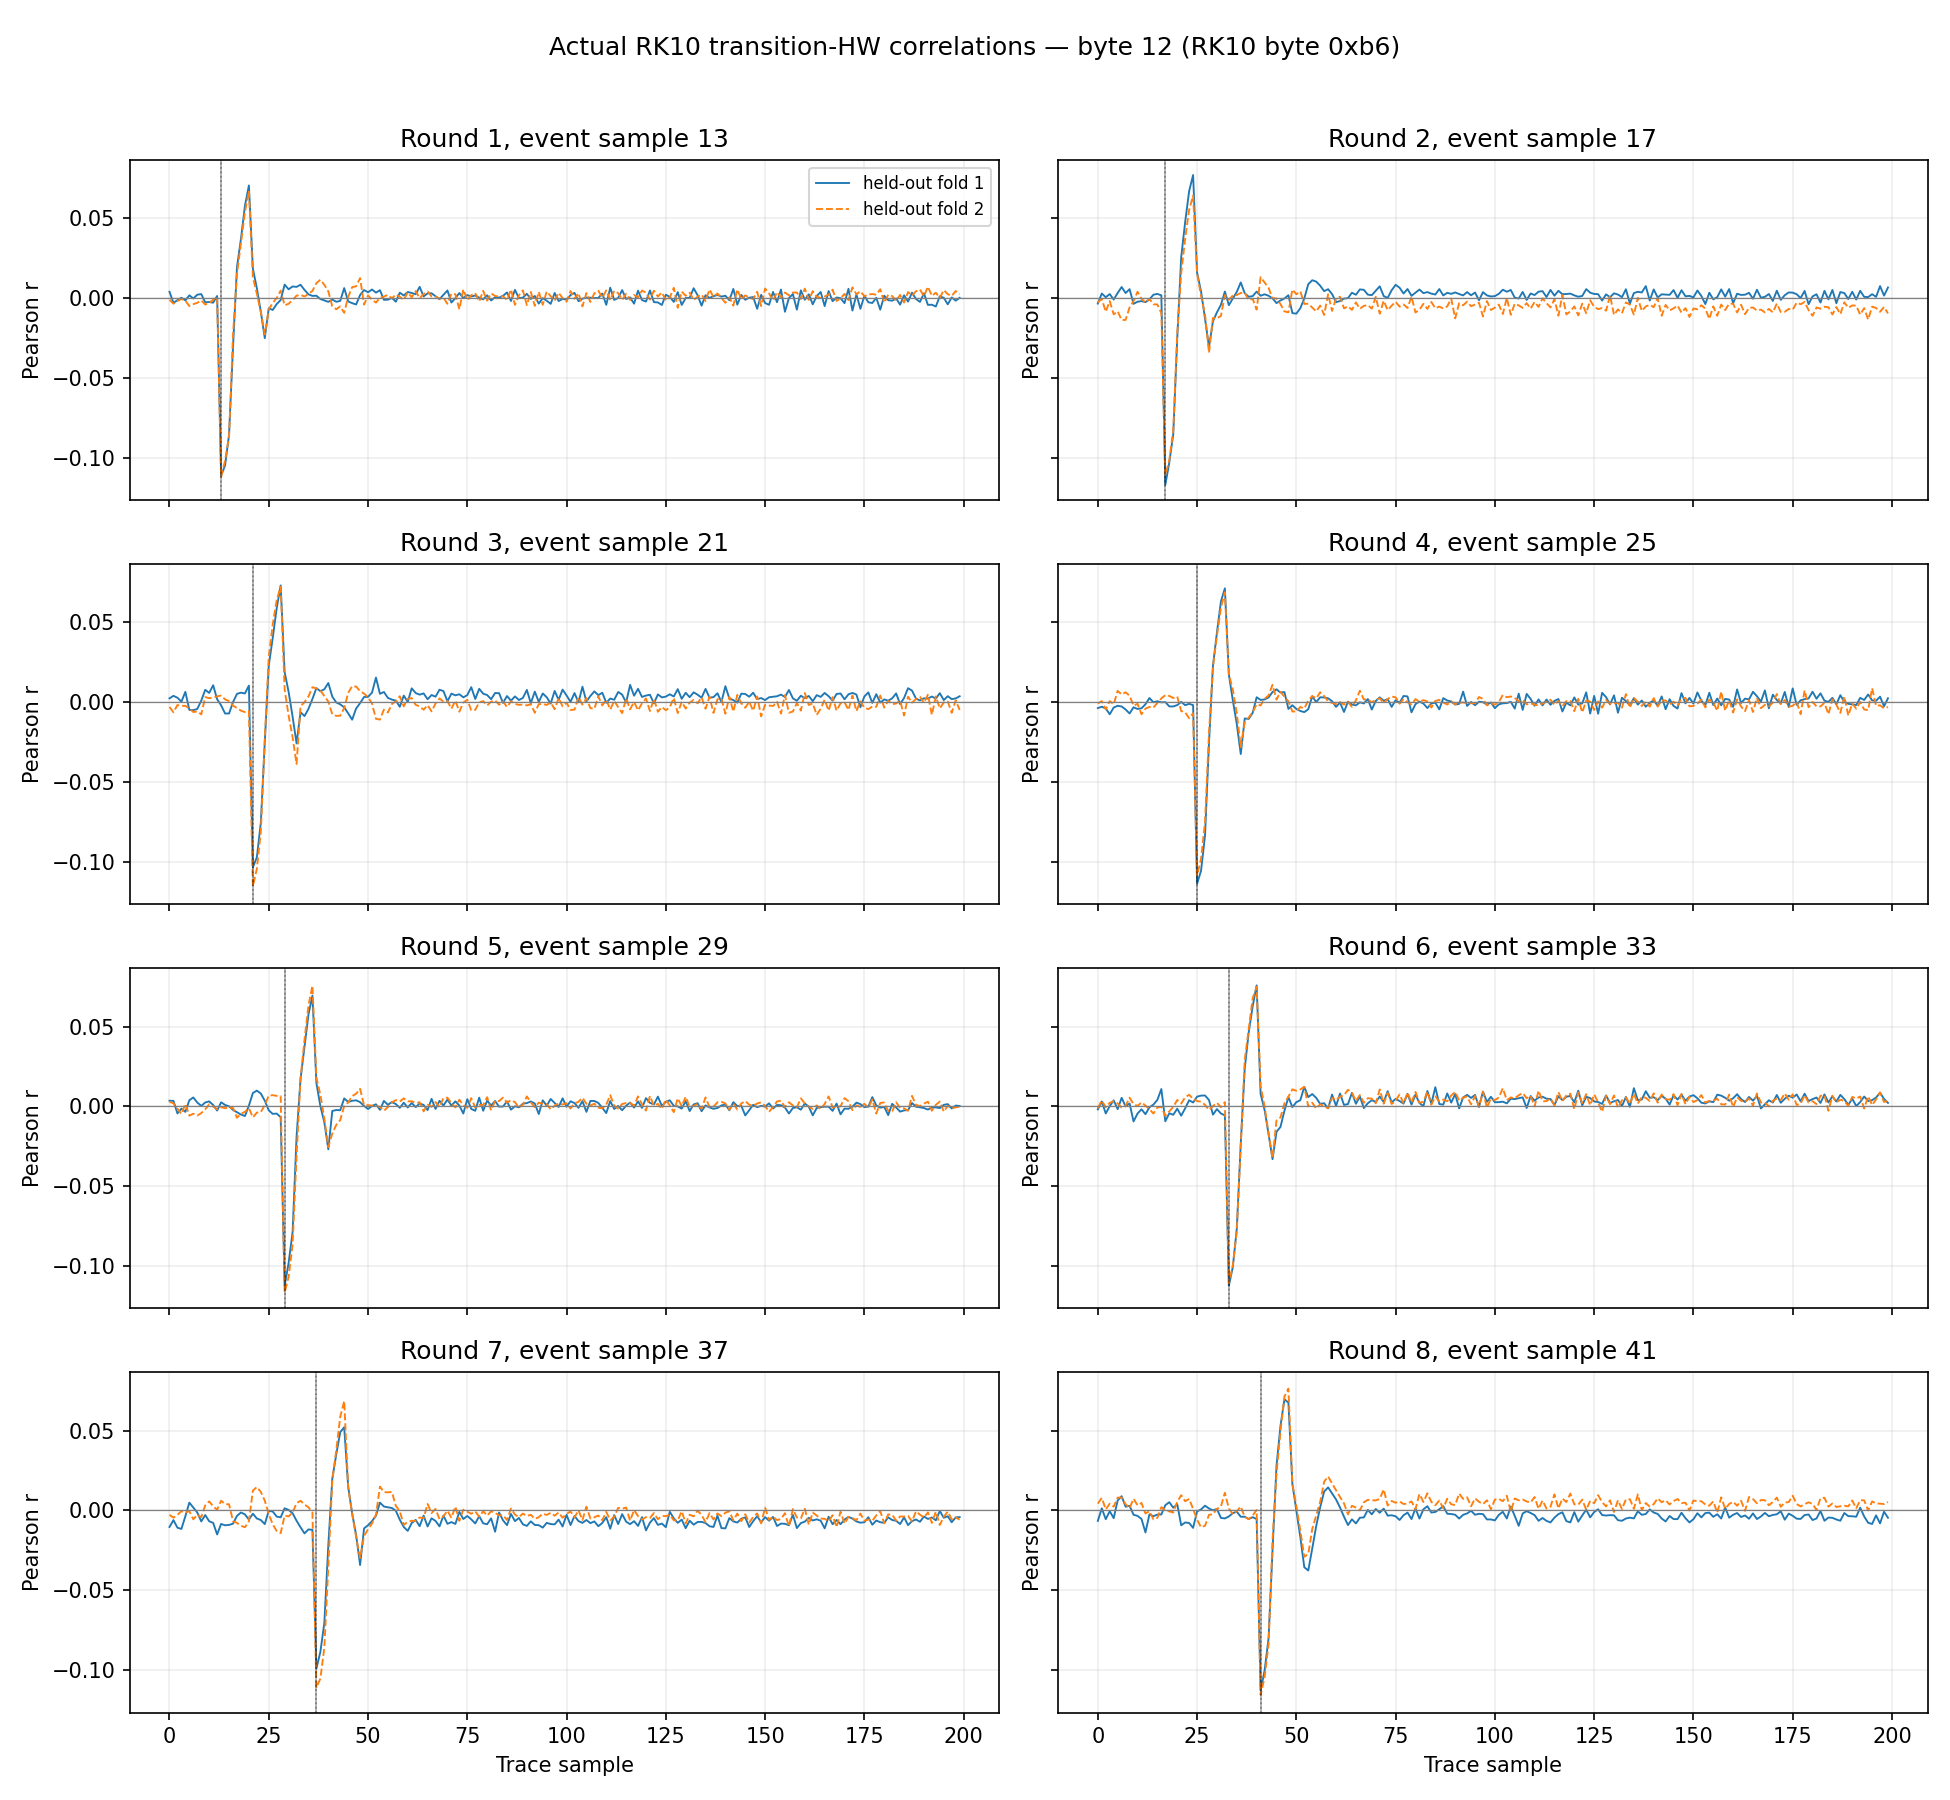
\includegraphics[width=0.96\textwidth]{actual_round10_correlation_plots/byte_12.png}
\caption{Task 3: endpoint-candidate correlations for byte 12 across rounds 1--8. Red curves mark the selected $z=\texttt{0xFF}$; dashed lines mark the detected event samples.}
\label{fig:task3-byte-12}
\end{figure}

\clearpage

\begin{figure}[H]
\centering
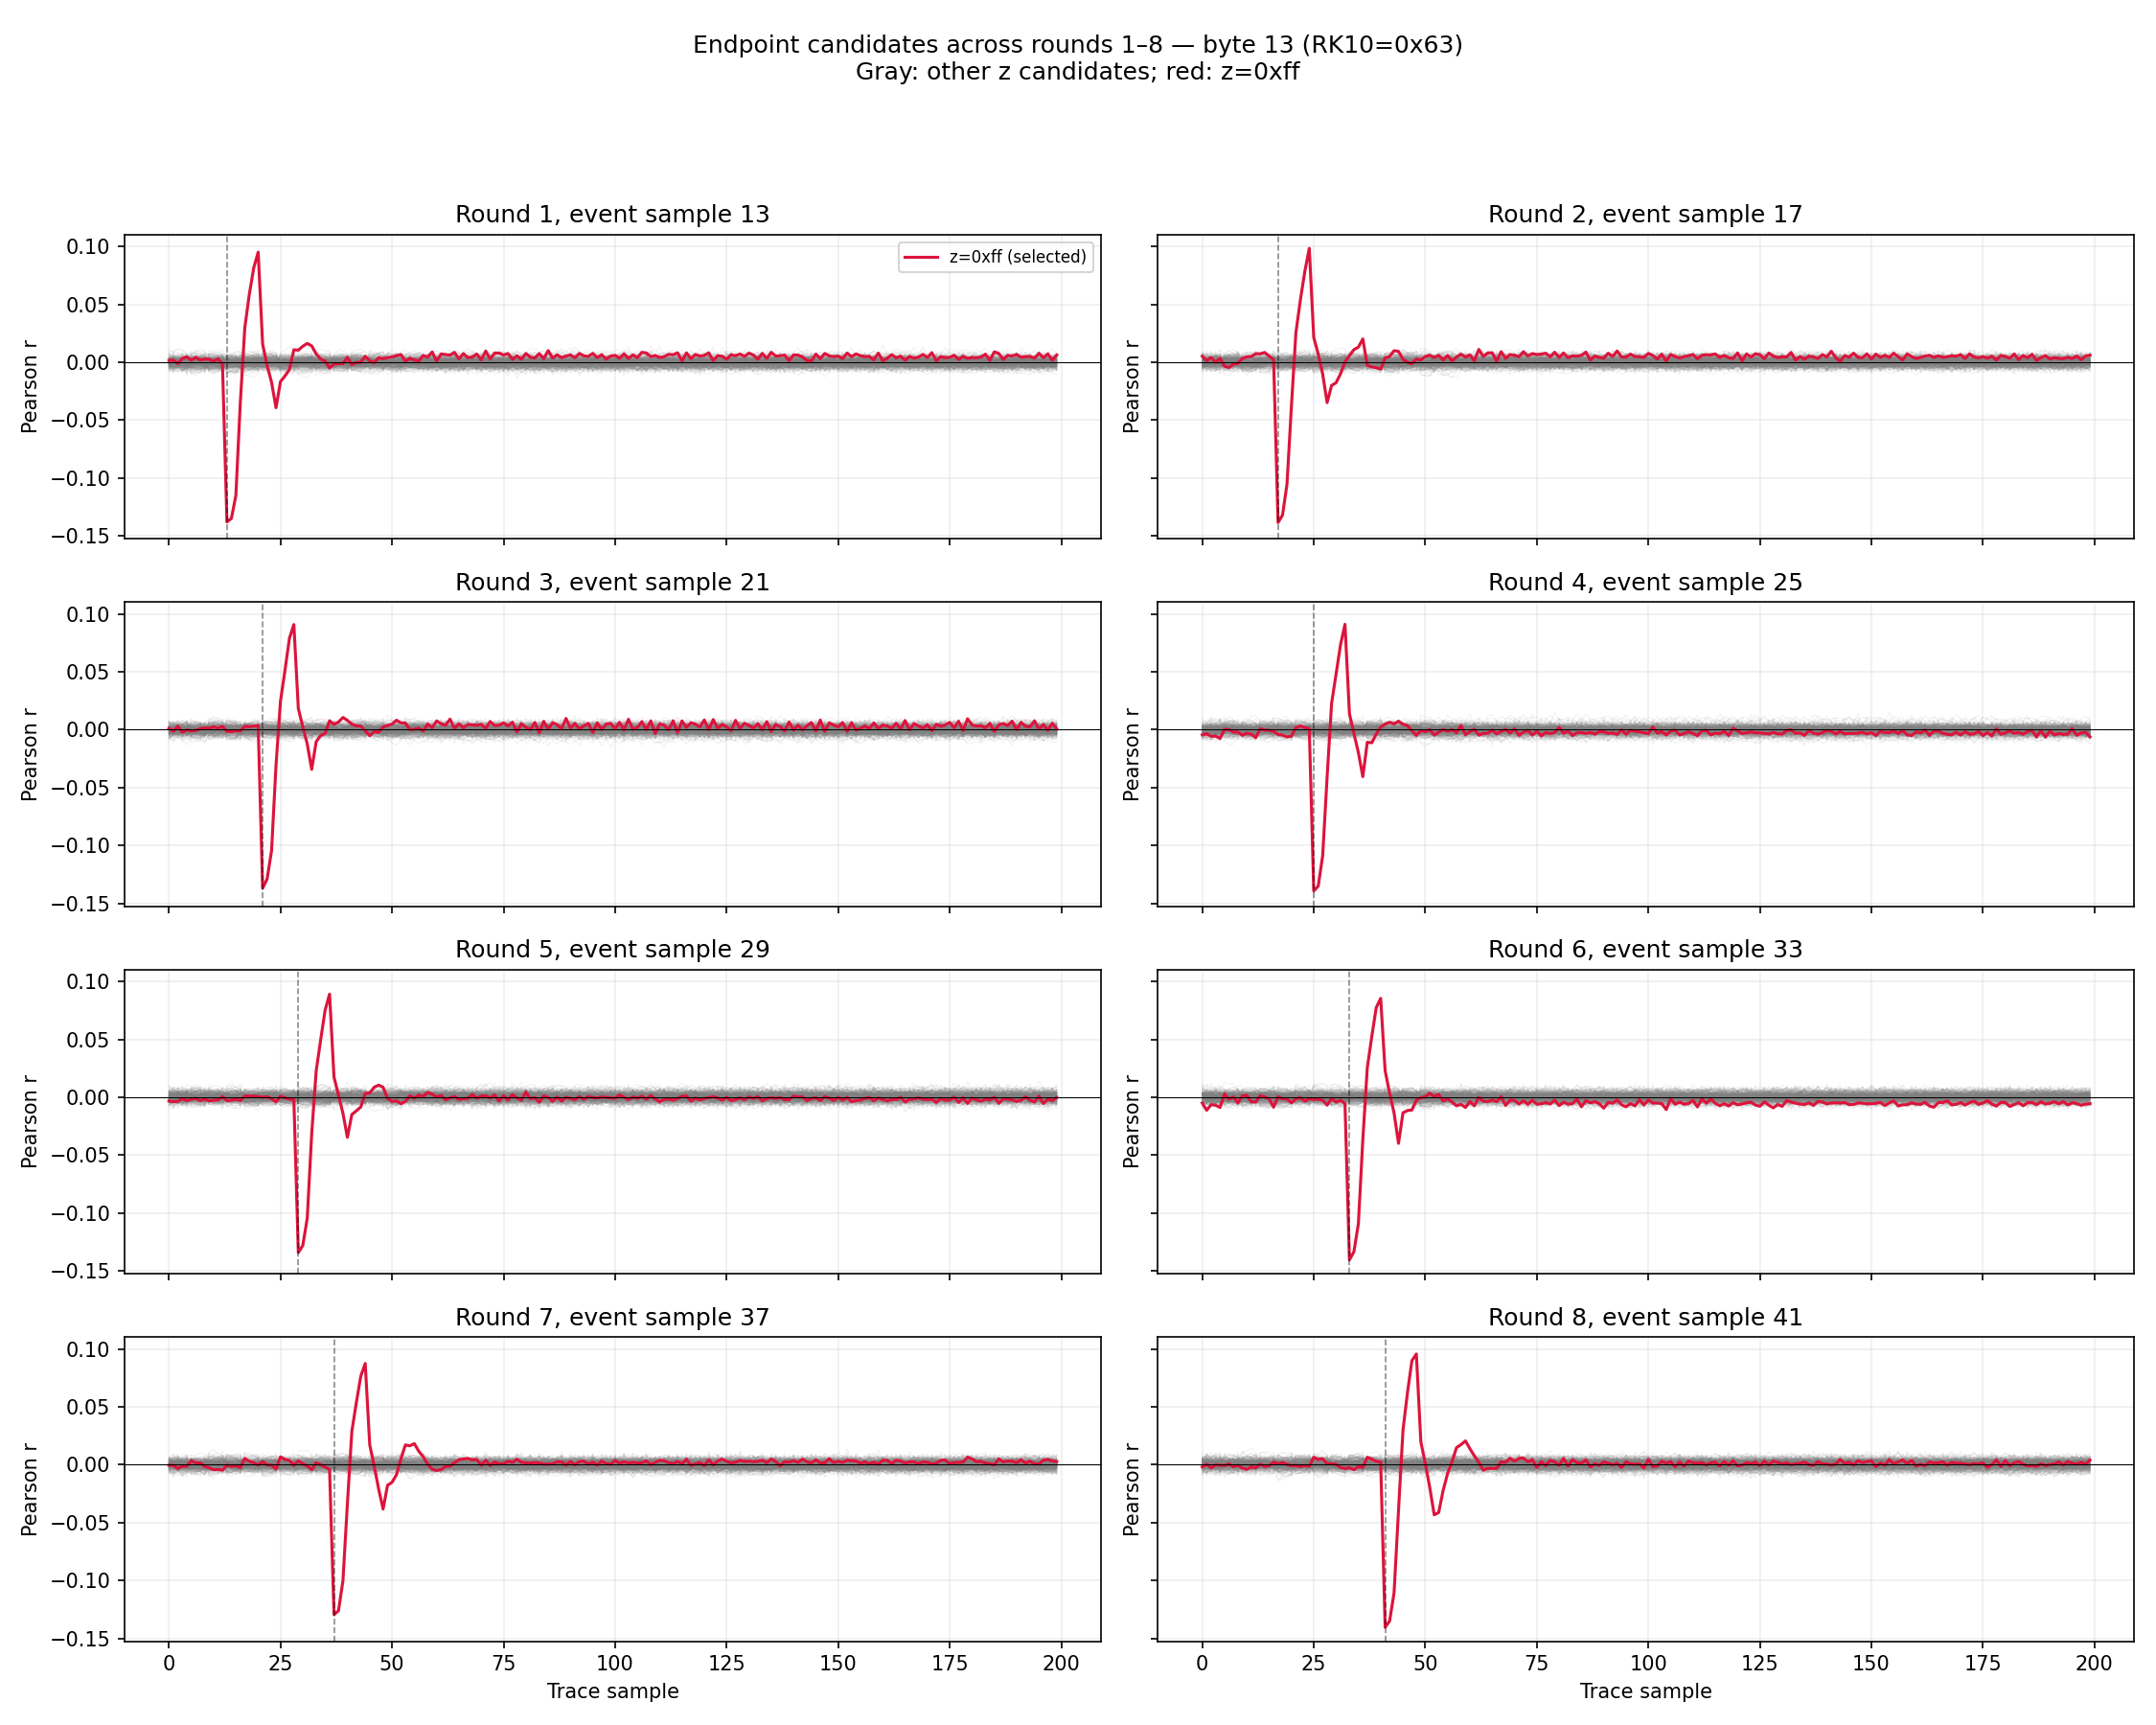
\includegraphics[width=0.96\textwidth]{actual_round10_correlation_plots/byte_13.png}
\caption{Task 3: endpoint-candidate correlations for byte 13 across rounds 1--8. Red curves mark the selected $z=\texttt{0xFF}$; dashed lines mark the detected event samples.}
\label{fig:task3-byte-13}
\end{figure}

\clearpage

\begin{figure}[H]
\centering
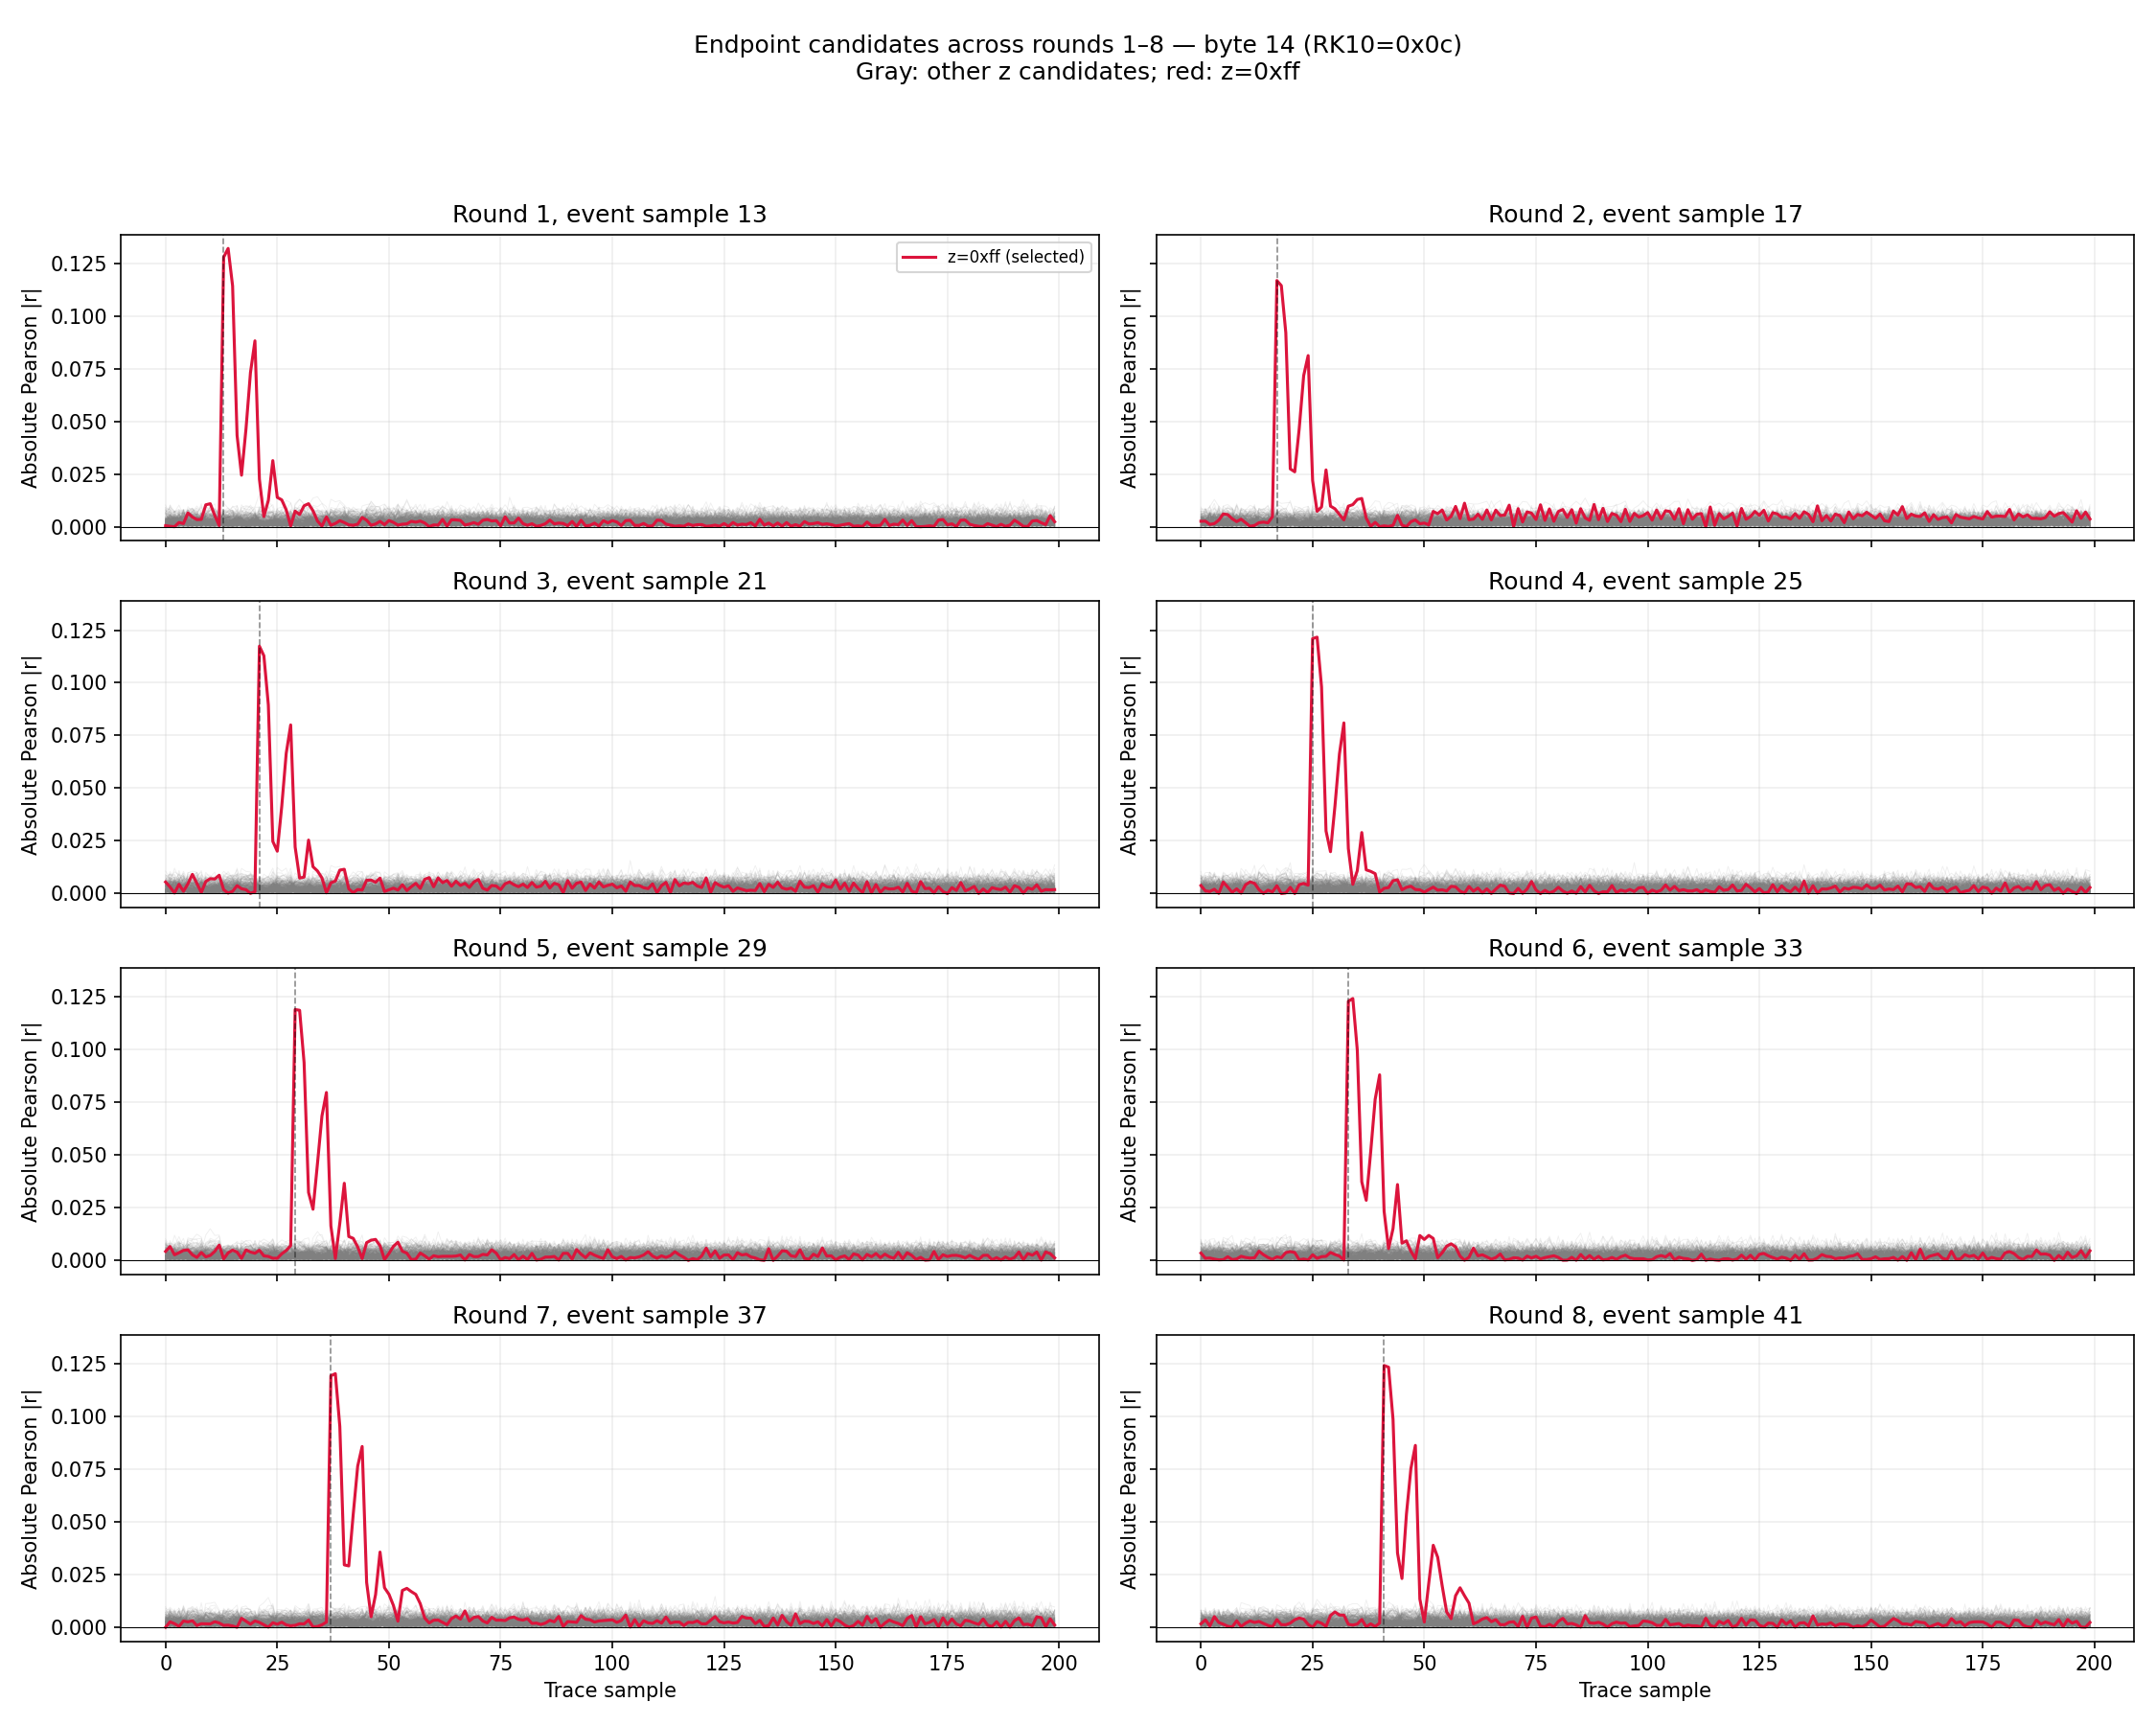
\includegraphics[width=0.96\textwidth]{actual_round10_correlation_plots/byte_14.png}
\caption{Task 3: endpoint-candidate correlations for byte 14 across rounds 1--8. Red curves mark the selected $z=\texttt{0xFF}$; dashed lines mark the detected event samples.}
\label{fig:task3-byte-14}
\end{figure}

\clearpage

\begin{figure}[H]
\centering
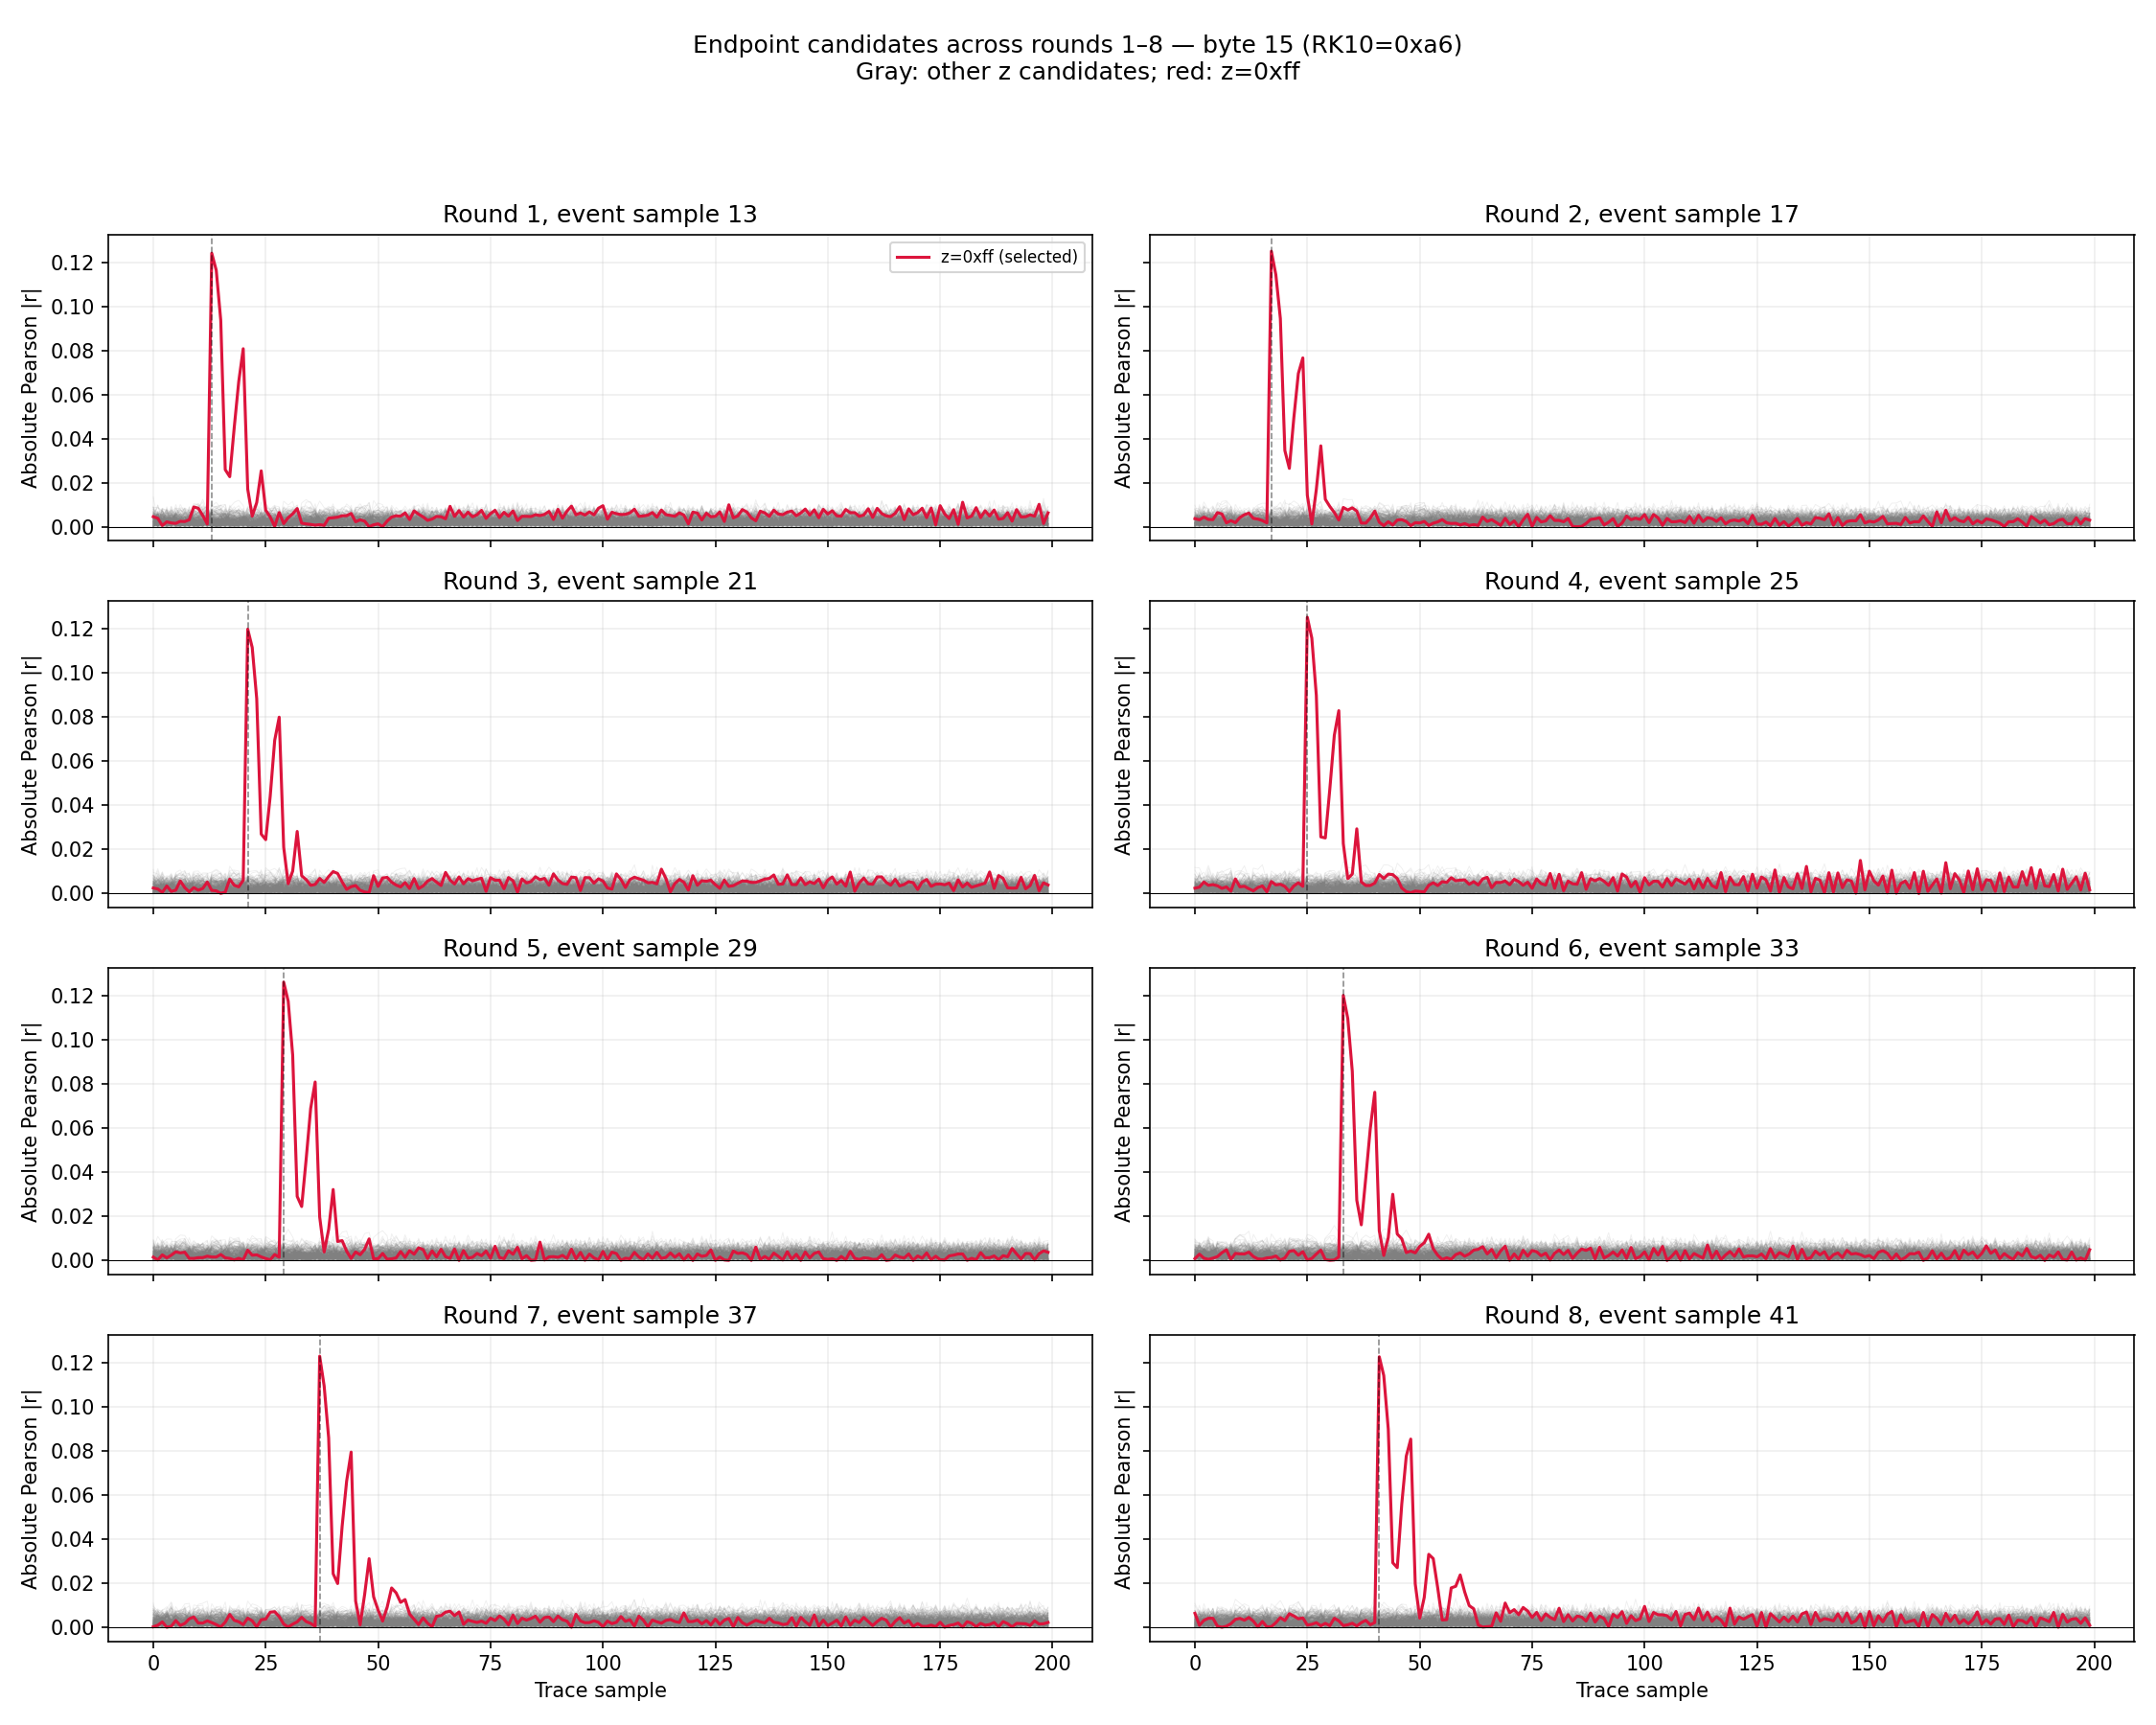
\includegraphics[width=0.96\textwidth]{actual_round10_correlation_plots/byte_15.png}
\caption{Task 3: endpoint-candidate correlations for byte 15 across rounds 1--8. Red curves mark the selected $z=\texttt{0xFF}$; dashed lines mark the detected event samples.}
\label{fig:task3-byte-15}
\end{figure}

\clearpage

